%%% thesis.tex 
%
% Robert Guderian, Sept 2000.
% Toyed with by John Anderson, 2002-2010, and likely by others not listed here as well.

%change to oneside if you want single sided.  Twoside will properly
%alternate margins and page numbers for two-sided binding.
%\documentclass[12pt,twoside,final]{huthesis}
\documentclass[12pt,singleside,final]{huthesis}


% change the font size of the captions
\usepackage[font=footnotesize,labelfont=bf]{caption}

%\usepackage{epsfig,bm,epsf,float}
\usepackage{graphicx}
\usepackage{algorithm,algorithmic}
%hyperref is nice, I find - it turns all your references (to citations, figures, etc) into hyperlinks,
% so someone reading electronically can jump around your document.  It makes no visible marks on a
%printed copy.
\usepackage[plainpages=false,breaklinks=true]{hyperref}

%use natbib for the bibliography
\usepackage[square,comma]{natbib}
%\bibpunct{[}{]}{;}{a}{,}{,} % this is just how natbib used to require options
%note, Natbib is not required for any thesis - avoid using it if you don't like it, but it provides many nice
%features for customizable bibliographies!

%%% Clear Header %%%%%%%%%%%%%%%%%%%%%%%%%%%%%%%%%%%%%%%%%%%%%%%%%%%%%%%%%%%%%%%%%%
% Clear Header Style on the Last Empty Odd pages
% this lets you jump to a new odd page (I have it set up for the end of the frontmatter)
% while ensuring the blank page that is left doesn't have a running header or anything, i.e. it's
% just completely blank. -JA (from Ki-Joo Kim, 2001)
    \makeatletter
    \def\cleardoublepage{\clearpage\if@twoside \ifodd\c@page\else%
        \hbox{}%
        \thispagestyle{empty}%
        \newpage%
        \if@twocolumn\hbox{}\newpage\fi\fi\fi}
    \makeatother

\def\newblock{\hskip .11em plus.33em minus.07em}

%% choose which files to process
%this was here to let you type in on the command line what you want TeX'd, and can be uncommented if you prefer to do it that way -
%but given that you'll probably have a number of chapters, it's much easier to just edit this
%file - JA
%\typein [\files]{Enter file names to process, (frontmatter,intro,
%  ...), or `all' to process all files:}
%\def\all{all}
%\ifx\files\all
%\typeout{Including all files.} \else \typeout{Including only \files.}
%\includeonly{\files}
%\fi

% Table of contents max depth listed:
% 1 = section, 2 = subsection, 3 = subsubsection
\setcounter{tocdepth}{2}

%added these to support better use of space re. figure placement - JA
\renewcommand{\floatpagefraction}{0.9}
\renewcommand{\topfraction}{0.9}
\renewcommand{\bottomfraction}{0.9}
\renewcommand{\textfraction}{0.1}


%import graphics drawing package
\usepackage{tikz}
\usetikzlibrary{positioning}

\usepackage{wrapfig}


% check which references are unused
% \usepackage{refcheck}

% for code prettification
\usepackage{listings}

% for making the tables have optional padding
\usepackage{array}

\begin{document}
%note that you can input your own additions if you want - here is an example from a previous
%user of this template.  I've left that math definition file in as it was supplied.
%%%% mathdefs.tex
%


% Taken from Adam Lupu-Sax ....................................................
%%% derivatives
\newcommand{\deriv}[2]{\frac{d#1}{d#2}}
\newcommand{\derivc}[3]{\left. \frac{d#1}{d#2}\right|_{#3}}
\newcommand{\pd}[2]{\frac{\partial #1}{\partial #2}}
\newcommand{\pdc}[3]{\left. \frac{\partial #1}{\partial #2}\right|_{#3}}

%%% Dirac notation
\newcommand{\bra}[1]{\left\langle #1\right|}
\newcommand{\ket}[1]{\left|#1\right\rangle}
\newcommand{\braket}[2]{\left\langle #1 \left|#2\right.\right\rangle}
\newcommand{\braOket}[3]{\left\langle #1\left|#2\right|#3\right\rangle}

% calligraphic letters in math.
\def\cal#1{\mathcal{#1}}


% Taken from M Haggerty ......................................................
\def\avg#1{\left< #1 \right>}
\def\abs#1{\left| #1 \right|}
\def\recip#1{\frac{1}{#1}}
\def\vhat#1{\hat{{\bf #1}}}
\def\smallfrac#1#2{{\textstyle\frac{#1}{#2}}}
\def\smallrecip#1{\smallfrac{1}{#1}}

% SPSmith's definitions ......................................................
\def\spshalf{{1\over{2}}}
\def\Orabi{\Omega_{\rm rabi}}
\def\btt#1{{\tt$\backslash$#1}}




% My own .....................................................................

%%% Equations
\def\schrod{Schroedinger's Equation}
\def\helm{Helmholtz Equation}


%%% Equation environments
\def\be{\begin{equation}}
\def\ee{\end{equation}}
\def\bea{\begin{eqnarray}}
\def\eea{\end{eqnarray}}
\def\bean{\begin{mathletters}\begin{eqnarray}}
\def\eean{\end{eqnarray}\end{mathletters}}


%%% macros for Feb 2000 PRL
\newcommand{\tbox}[1]{\mbox{\tiny #1}}
\newcommand{\half}{\mbox{\small $\frac{1}{2}$}}
\newcommand{\pit}{\mbox{\small $\frac{\pi}{2}$}}
\newcommand{\sfrac}[1]{\mbox{\small $\frac{1}{#1}$}}
\newcommand{\mbf}[1]{{\mathbf #1}}
% hack to get APS's \text style to work ok:
\def\text{\tbox}

\newcommand{\mV}{{\mathsf{V}}}
\newcommand{\mL}{{\mathsf{L}}}
\newcommand{\mA}{{\mathsf{A}}}
\newcommand{\lB}{\lambda_{\tbox{B}}}  % de Broglie
\newcommand{\ofr}{{(\mbf{r})}}       % (r vec)
\def\ofkr{(k;\mbf{r})}			% (k;r vec)
\def\ofks{(k;\mbf{s})}			% (k;s vec)
\newcommand{\ofs}{{(\mbf{s})}}       % (s vec)
\def\xt{\mbf{x}^{\tbox T}}		% x^T vec

\def\ce{\tilde{C}_{\tbox E}}		% C_E
\def\cew{\tilde{C}_{\tbox E}(\omega)}		% C_E(w)
\def\ceqmw{\tilde{C}^{\tbox{qm}}_{\tbox E}(\omega)}	% C^qm_E(w)
\def\cewqm{\tilde{C}^{\tbox{qm}}_{\tbox E}}	% C^qm_E(w) no omega
\def\ceqm{C^{\tbox{qm}}_{\tbox E}}	% C^qm_E no tilde
\def\cw{\tilde{C}(\omega)}		% C(w)
\def\cfw{\tilde{C}_{\cal F}(\omega)}		% C_F(w)

\def\tcl{\tau_{\tbox{cl}}}		% tau cl
\def\tcol{\tau_{\tbox{col}}}		% tau col
\def\terg{t_{\tbox{erg}}}		% t_erg
\def\tbl{\tau_{\tbox{bl}}}		% tau bl
\def\theis{t_{\tbox{H}}}		% t_Heis

\def\area{\mathsf{A}_D}			% piston effective area A_D 
\def\ve{\nu_{\tbox{E}}}			% nu_E, noise intensity
\def\vewna{\nu_E^{\tbox{WNA}}}		% nu_E for WNA

\def\dxcqm{\delta x^{\tbox{qm}}_{\tbox c}}	% x to mix levels.

%% operators
\newcommand{\rop}{\hat{\mbf{r}}}	% vector valued operators
\newcommand{\pop}{\hat{\mbf{p}}}


%%% Integrals
\newcommand{\sint}{\oint \! d\mbf{s} \,} % surface int
\def\gint{\oint_\Gamma \!\! d\mbf{s} \,} % surface int over Gamma.
\newcommand{\lint}{\oint \! ds \,}	% d=2
\def\infint{\int_{-\infty}^{\infty} \!\!}	% infinite integral
\def\dn{\partial_n}				% d_n
\def\aswapb{a^*\!{\leftrightarrow}b}		% a* <-> b
\def\eps{\varepsilon}				% eps

%%% Dissipation.
\def\dhdxt{\partial {\cal H} / \partial x}
\def\dhdx{\pd{\cal H}{x}}
\def\dhdxnm{\left( \pd{\cal H}{x} \right)_{\!nm}}
\def\dhdxnmsq{\left| \left( \pd{\cal H}{x} \right)_{\!nm} \right| ^2}

%%% vergini
\def\bcs{\stackrel{\tbox{BCs}}{\longrightarrow}}	% apply BCs




%%% DIEL atom project.
\def\wx{\omega_x}
\def\wy{\omega_y}
\newcommand{\ofro}{({\bf r_0})}
\def\Eb{E_{\rm blue,rms}}
\def\Er{E_{\rm red,rms}}
\def\Es2{E_{0,{\rm sat}}^2}
\def\sb{s_{\rm blue}}
\def\sr{s_{\rm red}}

%%% text usefuls
\def\ie{{\it i.e.\ }}
\def\eg{{\it e.g.\ }}
\newcommand{\etal}{{\it et al.\ }}
\newcommand{\ibid}{{\it ibid.\ }}

%%% tables spaces.
\def\gap{\hspace{0.2in}}


%%%%%%%%%%%%%%%%%%%%
%%% mathletters code (from http://www.grad.uiuc.edu/thesis/latexcode.html )
% Modified Alex Barnett 00/9/28 to handle non-arabic \thechapter output
% (ie, now works in Appendices)
% Fails to give correct references in eqnarray (offset by one).
% Still inserts small extra space after equation - unknown reason.
%
%    Original code:
%\newcounter{eqletter}
%\def\mathletters{%
%\setcounter{eqletter}{0}%
%\addtocounter{equation}{1}
%\edef\curreqno{\arabic{equation}}
%\edef\@currentlabel{\theequation}
%\def\theequation{%
%\addtocounter{eqletter}{1}\arabic{chapter}.\curreqno\alph{eqletter}%
%}%
%}
%\def\endmathletters{\setcounter{equation}{\curreqno}}

\newcounter{eqletter}
\def\mathletters{%
\setcounter{eqletter}{0}%
\addtocounter{equation}{1}
\edef\curreqno{\arabic{equation}}
\edef\@currentlabel{\theequation}
\def\theequation{%
\addtocounter{eqletter}{1}\thechapter.\curreqno\alph{eqletter}%
}%
}
\def\endmathletters{\setcounter{equation}{\curreqno}}


%...............................................QPC...................

\newcommand{\bk}{{\bf k}}
\def\kf{k_{\text F}}
\newcommand{\br}{{\bf r}}
\newcommand{\TL}{{\text{(L)}}}
\newcommand{\TR}{{\text{(R)}}}
\newcommand{\TLR}{{\text{L,R}}}
\newcommand{\VSD}{V_{\text{SD}}}
\newcommand{\GT}{\Gamma_{\text{T}}}
\newcommand{\DEL}{\mbox{\boldmath $\nabla$}}
\def\lf{\lambda_{\text F}}
\def\st{\sigma_{\text T}}
\def\stlr{\sigma_{\text T}^{\text{L$\rightarrow$R}}}
\def\strl{\sigma_{\text T}^{\text{R$\rightarrow$L}}}
\def\aeff{a_{\text{eff}}}
\def\aaeff{A_{\text{eff}}}
\def\gat{G_{\text{atom}}}
\newcommand{\LB}{Landauer-B\"{u}ttiker}

% .............. NOTES ..................
% To force linebreak when get overfull hbox from equation in paragraph
% test, use \linebreak (which makes it justify the line it broke).
% Contrast \\ or \newline which leave empty space.
%
%
 % my math definitions.

% UNDERLYING SPACING FOR WHOLE DOCUMENT:
% Single spacing: takes place of `draft' mode, without losing figures.
% \ssp

% makes double-spaced
\dsp


\title{Intelligent Clustering in Wireless Sensor Networks}%
\author{Robert William Lee Guderian}

\degreemonth{July} % month final submission occurs.
\degreeyear{2012}%
\degree{Master of Science}%
\department{Computer Science}%
\advisor{Dr.\ Rasit Eskicioglu} %


%\copyrightpage
% Insert a blank page for two-sided
%  \newpage
%  \thispagestyle{empty}
%  \hbox{}
%  \newpage


\maketitle

\begin{abstract}

	Wireless Sensor Networks (WSNs) are networks of small devices, called motes,
    	designed to monitor resources and report to a server. Motes are 
    	battery-powered and have very little memory to store data. To conserve power, 
    	the motes usually form clusters to coordinate their activities. In 
    	heterogeneous WSNs, the motes have different resources available to them. For 
    	example, some motes might have more powerful radios, or larger power supplies. 
    By exploiting heterogeneity within a WSN can allow 
    	the network to stay active for longer periods of time.

    	In WSNs, the communications between motes draw the most power. By choosing 
    	better clusterheads in the clusters to control and route 
    	messages, all motes in the network will have longer lifespans. By leveraging 
    	heterogeneity to select better clusterheads, I have developed
    	Heterogeneous Clustering Control Protocol (HCCP). HCCP is designed to be 
    	highly robust to change and to fully utilize the resources that are currently 
    	available.

    


\end{abstract}

\newpage
\tableofcontents

\addcontentsline{toc}{section}{Table of Contents}
%comment these out if you don't want a detailed list of figures and tables!
\listoffigures
\listoftables

\begin{acknowledgments}
I would like to begin by thanking my Dr.\ Rasit Eskicioglu who has been my
long-suffering advisor to whom I will forever be grateful. I'd like to thank
my committee, Dr.\ Peter Graham and Dr.\ Bob McLeod for all their input
and patience. I'd finally like to thank my biggest fan, my inspiration, my
editor, my best friend and wife, Becky.
\end{acknowledgments}

%
\dedication
\begin{quote}
\hsp \em \raggedleft Dedicated to Becky for always believing in me.
\end{quote}

%\newpage
\cleardoublepage
\thispagestyle{empty}
\startarabicpagination

%%% end


% Chapters: list all the chapter latex files you want included here, in order

% subsections are grouped with the title of the chapter
\chapter{Introduction}
\label{ch:ch1}

A Wireless Sensor Network (WSN) is a network of many small, battery-powered 
devices, called motes,  that create ad-hoc networks via wireless radios.  
Motes are inexpensive devices outfitted with various sensors and are configured to 
monitor some phenomena and report back to a server -- called a sink. 
Estrin et al.~\cite{nextCentury} 
elegantly described WSNs as,
\begin{quote}
	``...sensors only interact with other sensors in a restricted 
	vicinity, but nevertheless collectively achieve a desired 
	global objective."
\end{quote}
This captures the essence of a WSN concisely, describing the 
multi-hop environment and how a WSN consists of many small objects 
that are working towards a larger goal.

\begin{figure}[htbp]
	\centering
		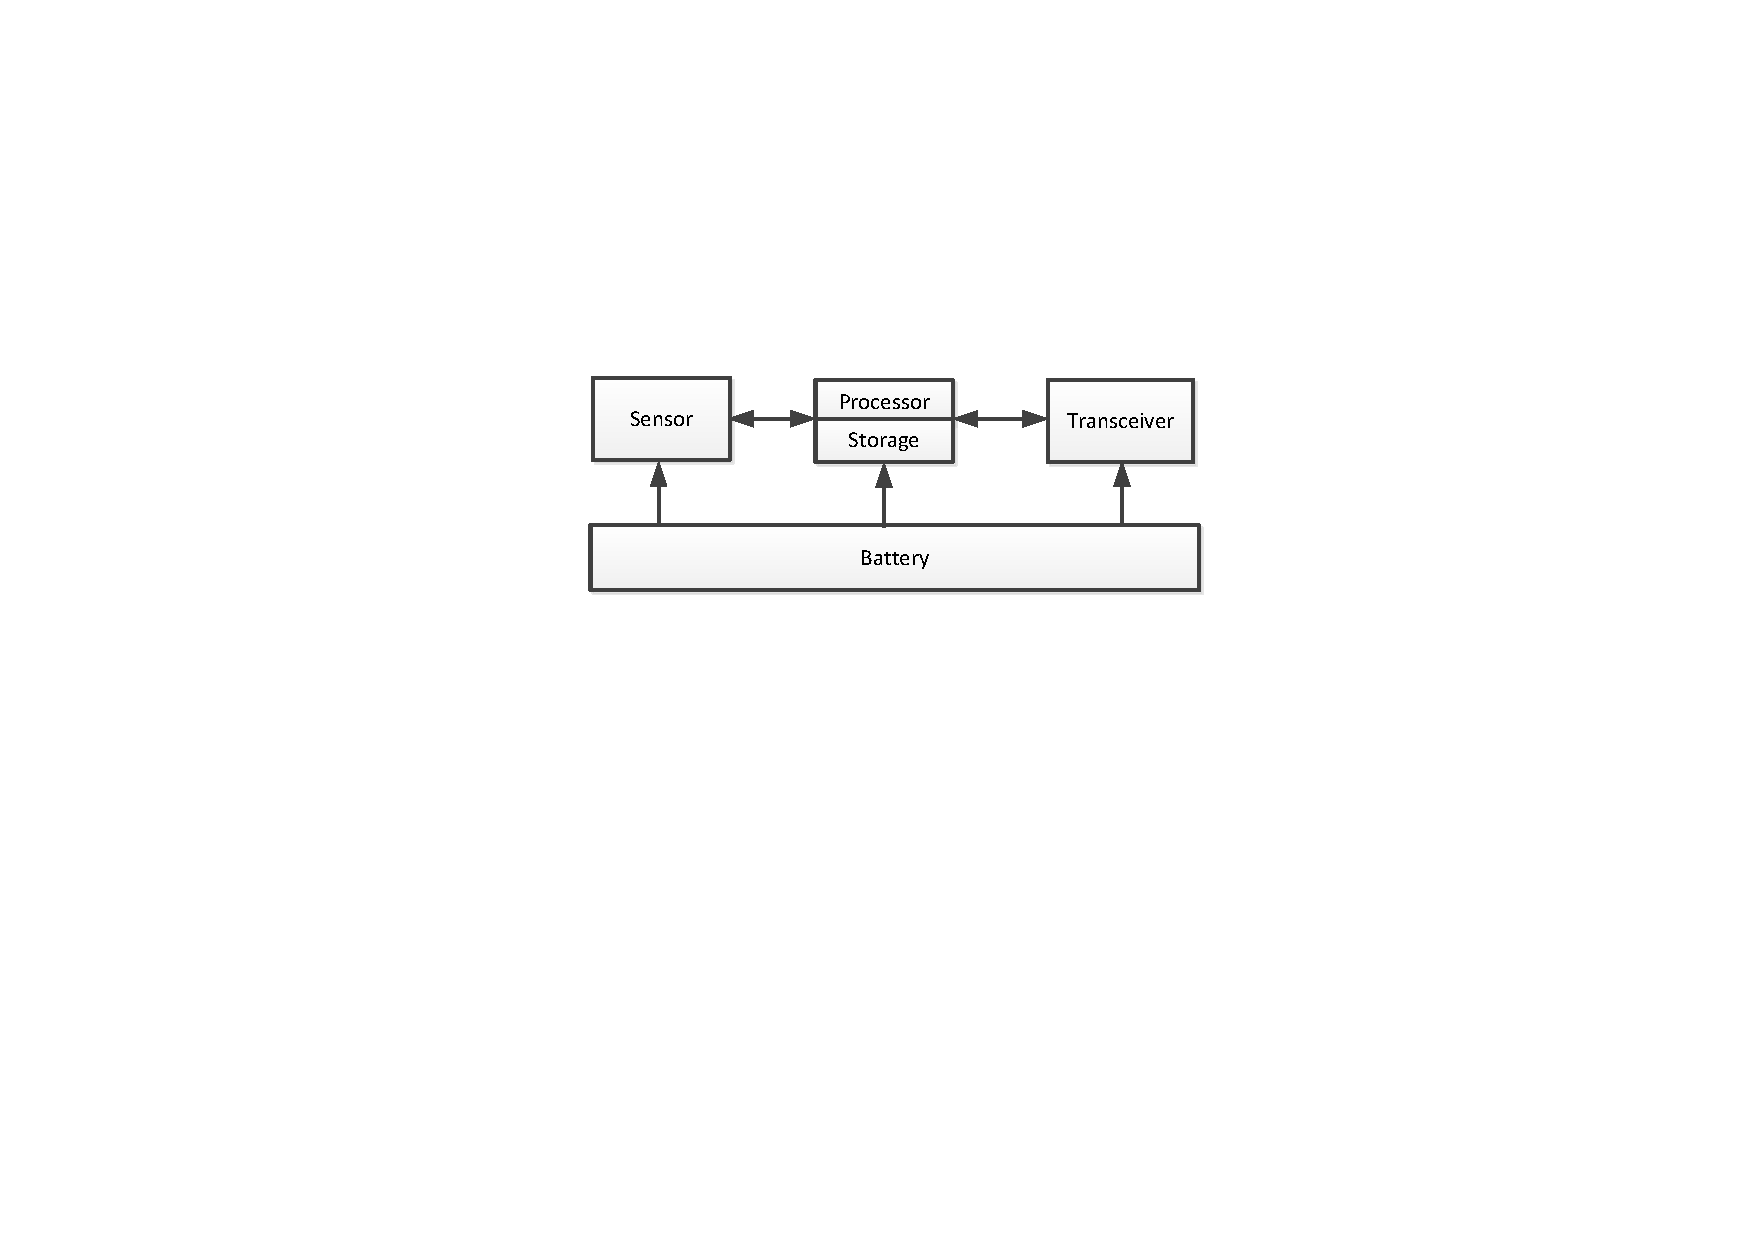
\includegraphics[width=4.5in]{images/intro/mote.pdf}
	\caption{High-level description of a mote. Adapted from ~\cite{wsnSurvey}.}
	\label{fig:images_intro_mote}
\end{figure}

Motes are simple devices that have very few components. 
Motes consist of a battery for power, sensors for
detecting some phenomena, memory for storing the
data collected, a radio for communication and a processor for 
controlling all the other components. Optionally motes
can have ways to regenerate power, such as a solar panel, and 
some motes have the ability to move. The layout of a mote can be seen
graphically in Figure~\ref{fig:images_intro_mote}. 




Applications for WSNs range from animal habitat monitoring~\cite{duckisland,zebranet}
to building and bridge structural monitoring~\cite{StructuralMonitoring}, to 
monitoring live volcanoes during eruptions~\cite{volcano}. 
Typically, when deployed, a WSN self-configures, creating routes from sensor 
motes to the sink automatically. 
Most routes in WSNs are not direct to the sink, therefore motes must use 
several peer motes as a multi-hop network to send messages to the sink.
Routing protocols in WSNs must automatically create these multi-hop routes to 
form a functioning network.
To create these routes, routing algorithms designed for WSNs, such as the
Collection Tree Protocol~\cite{ctp} are used.

There are many scenarios where a WSN could be used to make a task 
simpler, or even save lives.
For instance, Werner-Allen et al.~\cite{volcano} have used a WSN to monitor
a seismic and infrasonic (low-frequency acoustic)  volcanic eruption. The team wanted to have as many motes as possible, and
as long a network lifespan to collect as much data as possible. Every project 
has a limited budget, and high-powered radios are expensive and use lots of energy. 
Since high-powered radios were ruled out, Werner-Allen et al.\ chose to use
a multi-hop WSN. A WSN allowed the team to deploy many sensors with low-power radios 
that could communicate their findings back to the computer they used as a sink. 
Some sensors were lost during the eruption, which could have meant a loss of life or a loss of data
if the sensors required people to continually check them. Since a WSN was
used, the data was transferred off the mote before it was lost to the eruption and provided some
very interesting data!

\begin{wrapfigure}{r}{8cm}
    \fbox{
    \begin{minipage}{7.5 cm}
    
        \begin{center}    
          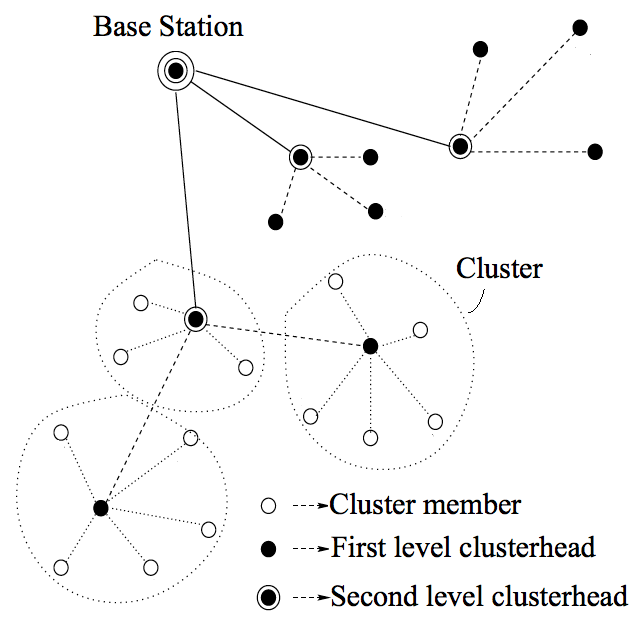
\includegraphics[width=7cm]{images/intro/clusters.png}
        \end{center}
        \caption{A hierarchical cluster topology~\cite{teen}. }
        \label{photo}
    \end{minipage}
    }
  \end{wrapfigure}

WSNs can also be used in less exciting work, such as bridge or vehicle monitoring~\cite{StructuralMonitoring}.
If it is difficult or inconvenient for a person to check strain levels on bridges, a WSN
can be deployed to monitor the bridge. Some of these bridges can be difficult to get power to, as
they might be far into a forest or in a remote location. A battery-powered WSN does not require 
external power to be run to the area, and can continually monitor strain levels without human intervention,
saving companies or governments time and money while making the structure safer.
  
To simplify routing  and to conserve energy, a WSN  groups motes into 
clusters. These clusters elect a clusterhead which works as a gateway and 
routes all network traffic in and out of the cluster. Motes that are cluster 
members only communicate with the clusterhead. Clusterheads then route the 
messages though other clusterheads, to the sink. An example of this can be 
seen in Figure~\ref{photo}.  This simplifies the network topology as each cluster 
can be viewed as one large mote.  Messages to the sink are then routed through 
clusterheads only, which lowers the number of hops taken from the originating 
cluster to the sink. Using clusterheads reduces the energy draw from all motes 
that are in the cluster since they only need to send messages to the 
clusterhead. The clusterhead accepts messages from the motes in the cluster, 
creates one large message out of all the messages, and sends this large 
message to the sink. Handling messages in this way allows motes that are 
cluster members to sleep or be idle while the clusterhead attempts to send the 
message across the network, thus saving power.


A heterogeneous WSN has motes that are not all identical. There may be several 
different types of motes from different companies or motes from the same 
company with different characteristics.  Motes may be running different 
operating systems, be programmed with different software or have additional 
hardware. Homogeneous networks can also be viewed as heterogeneous 
networks; heterogeneity occurs as motes change over time, such as a mote's 
battery depletion or a mote malfunctioning. These differences, large and 
small, can be exploited to extend the network lifespan or increase message throughput.  

In a WSN, typically 
%motes can be specialized to a task to provide more detailed information about the resource it is monitoring.
a mote is assigned to provide detailed information about the phenomenon it is 
monitoring. 
If a few motes are equipped with more expensive hardware, the network should 
adapt to allow these motes to live longer. This can be done by not allowing 
the more expensive mote to be a clusterhead, and by providing a clusterhead 
in range of the expensive mote.
As this specialization increases, so does the heterogeneity of the network. 
Clusterheads should be selected to allow the specialized motes to have  
longer lifespans. Or, if a mote has a larger available message queue it should be
elected to be a clusterhead since it will be less likely to lose messages
if a large number of messages are sent to it, making the mote a good message routing mote.

% redundant?
%The network must be aware of the resources to each mote and select clusterheads within radio range of these motes. In a highly specialized heterogeneous network, clusterheads must be chosen to allow all the specialized motes to communicate with the sink to ensure both network lifetime is long and messages from the motes get to the sink.

A `long-lived WSN' is a network that is designed to stay active for extended 
periods of time. Long-lived WSNs use techniques such as duty cycling and make 
as few transmissions as possible to achieve longer network lifespan. It is 
difficult to have a long-lived network mostly due to the battery-powered 
nature of motes. Long-lived networks often trade off some functionality, such 
as the frequency of sampling with their sensors and the frequency of 
reporting,  to increase mote lifespan.

A clusterhead is a mote that controls transmissions from other 
motes in the immediate neighbourhood. Clusterhead motes draw more power due to 
the increased number of transmissions they perform as they must stay active to receive messages 
from the cluster. 
The key to long-lived networks is selecting motes that are well-suited to be clusterheads.  
Therefore, in a 
heterogeneous long-lived WSN, motes that have more or larger batteries and have plenty 
of residual energy should be elected to be clusterheads. If the 
clusterhead has little power left or has a malfunctioning radio, the 
probability of losing messages increases. Using heterogeneity to avoid 
choosing a mote that is better designed to be a clusterhead will aid in 
designing a long-lived network.

Suitable clusterheads are important when building a long-lived WSN. The 
clusterhead draws a large amount of power, therefore  the performance of 
clusterhead motes will degrade over time. If a clusterhead mote detects that 
it is performing poorly (e.g., cannot keep up handling the incoming messages 
from their motes), it should opt-out or demote itself to pass the task on to a 
more capable mote. Passing the clusterhead task to a more capable mote will 
prevent the poorly-performing mote from losing transmissions and causing 
retransmissions, which creates unnecessary overhead in the surrounding motes.

To increase message throughput, extend lifespans of individual motes and allow WSNs to function longer, I 
have developed Heterogeneous Clustering and Control Protocol (HCCP). HCCP 
uses a taxonomy to describe heterogeneity and selects candidate clusterheads 
based on the capabilities of motes.





\chapter{Related Work}
\label{ch:related}

Many researchers have contributed to the WSN field, all focusing on different areas.
There are a few different aspects of WSNs that are considered in this thesis. To reflect this, the 
related work is grouped by different areas of WSN research. 

Areas
of WSN research include radio transceiver technology which has been 
developed for decades, but has only recently been developed as a low-power
technology. WSN research also includes MAC layer protocols, which are used by radios to share 
a radio channel between multiple devices. 
To move messages towards the sink, WSN nodes can either create 
clusters (Clustering Protocols), or communicate without clusters (Non-clustering Protocols).
There are benefits to using clusters in WSNs, and other benefits to not using clusters. 
Finally, heterogeneity in WSNs can be used
to improve the performance of a WSN.


\section{Wireless Sensor Networks}

% http://en.wikipedia.org/wiki/History_of_radio
Wireless technologies are by no means a new invention. In 1892
Nikola Tesla proposed that radio waves could be used for communication
without any wires connecting the two points~\cite{telsa}.
Since then, wireless radios have evolved from large, power 
hungry devices such as radio backpacks used in World War II, to 
%http://www.ww2gyrene.org/equipment_SCR_300.htm
%\begin{figure}[htbp]
%    \centering
%        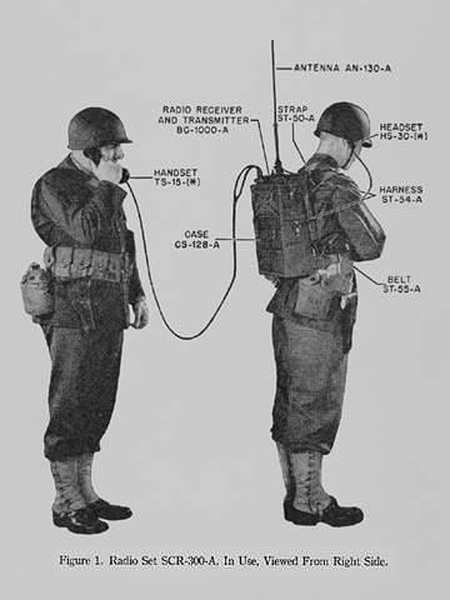
\includegraphics[height=3in]{images/relatedWork/Scr300.png}
%    \caption{A backpack radio as used in World War II. (Image via PD-USGOV)}
%    %http://en.wikipedia.org/wiki/File:Scr300.png
%    \label{fig:images_relatedWork_Scr300}
%\end{figure}
the ubiquitous cell phone of today. Wireless radios have gotten smaller,
more power efficient and much more affordable. 

The story of the computer has much in common with the evolution of the 
wireless radio. Starting with computers that were large and extremely expensive, 
computers are now standard equipment for everyday use. The
cost of computers has gone way down, as has the size of computers. Both wireless
radios and computer are core components of WSN nodes.

The paper that is often credited in being the first paper on designing WSNs is 
Pottie and Kaiser's~\cite{WINSProject}  \emph{Wireless Integrated Network Sensors}.
Pottie and Kaiser proposed the acronym WINS for the field, and were the first
to connect the ideas of pervasive low power computing with sensor networks and proposed an
architecture to help solve these problems. 
At its core WSNs are just microcontrollers, sensors and 
wireless radios; Pottie and Kaiser saw the potential of these
objects, and showed the world that the combination is more than the sum of its parts. 
The authors moved beyond looking at the components, and considered what could be possible
with the concept, and how it would need to be achieved. Pottie and Kaiser 
saw that the density of the distributed network is the strength of WSNs. Key points of the 
paper were that using the shortest transmission range is important
to increase node lifespan, and that networks must be self-organizing to work efficiently.

\begin{figure}[tb]
	\centering
		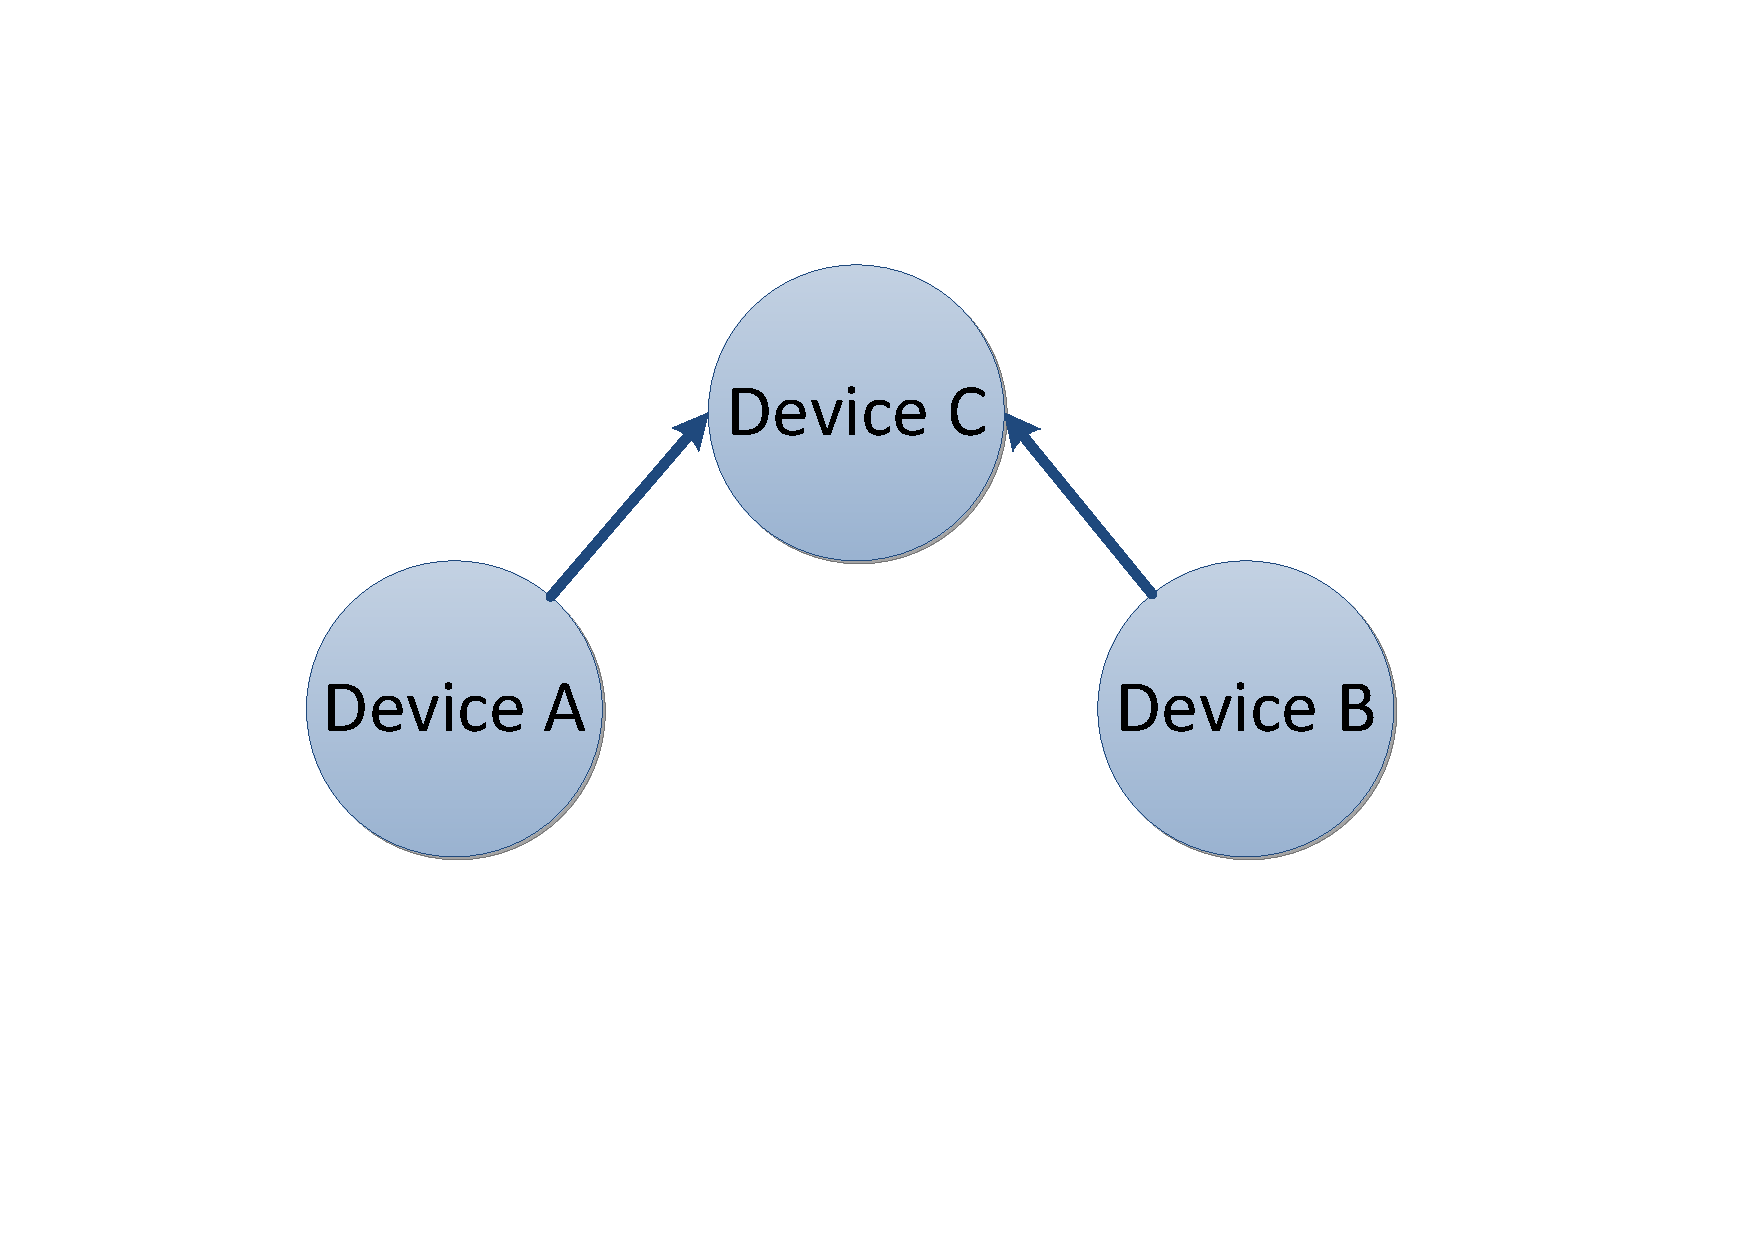
\includegraphics[width=3in]{images/relatedWork/HiddenNode.pdf}
		%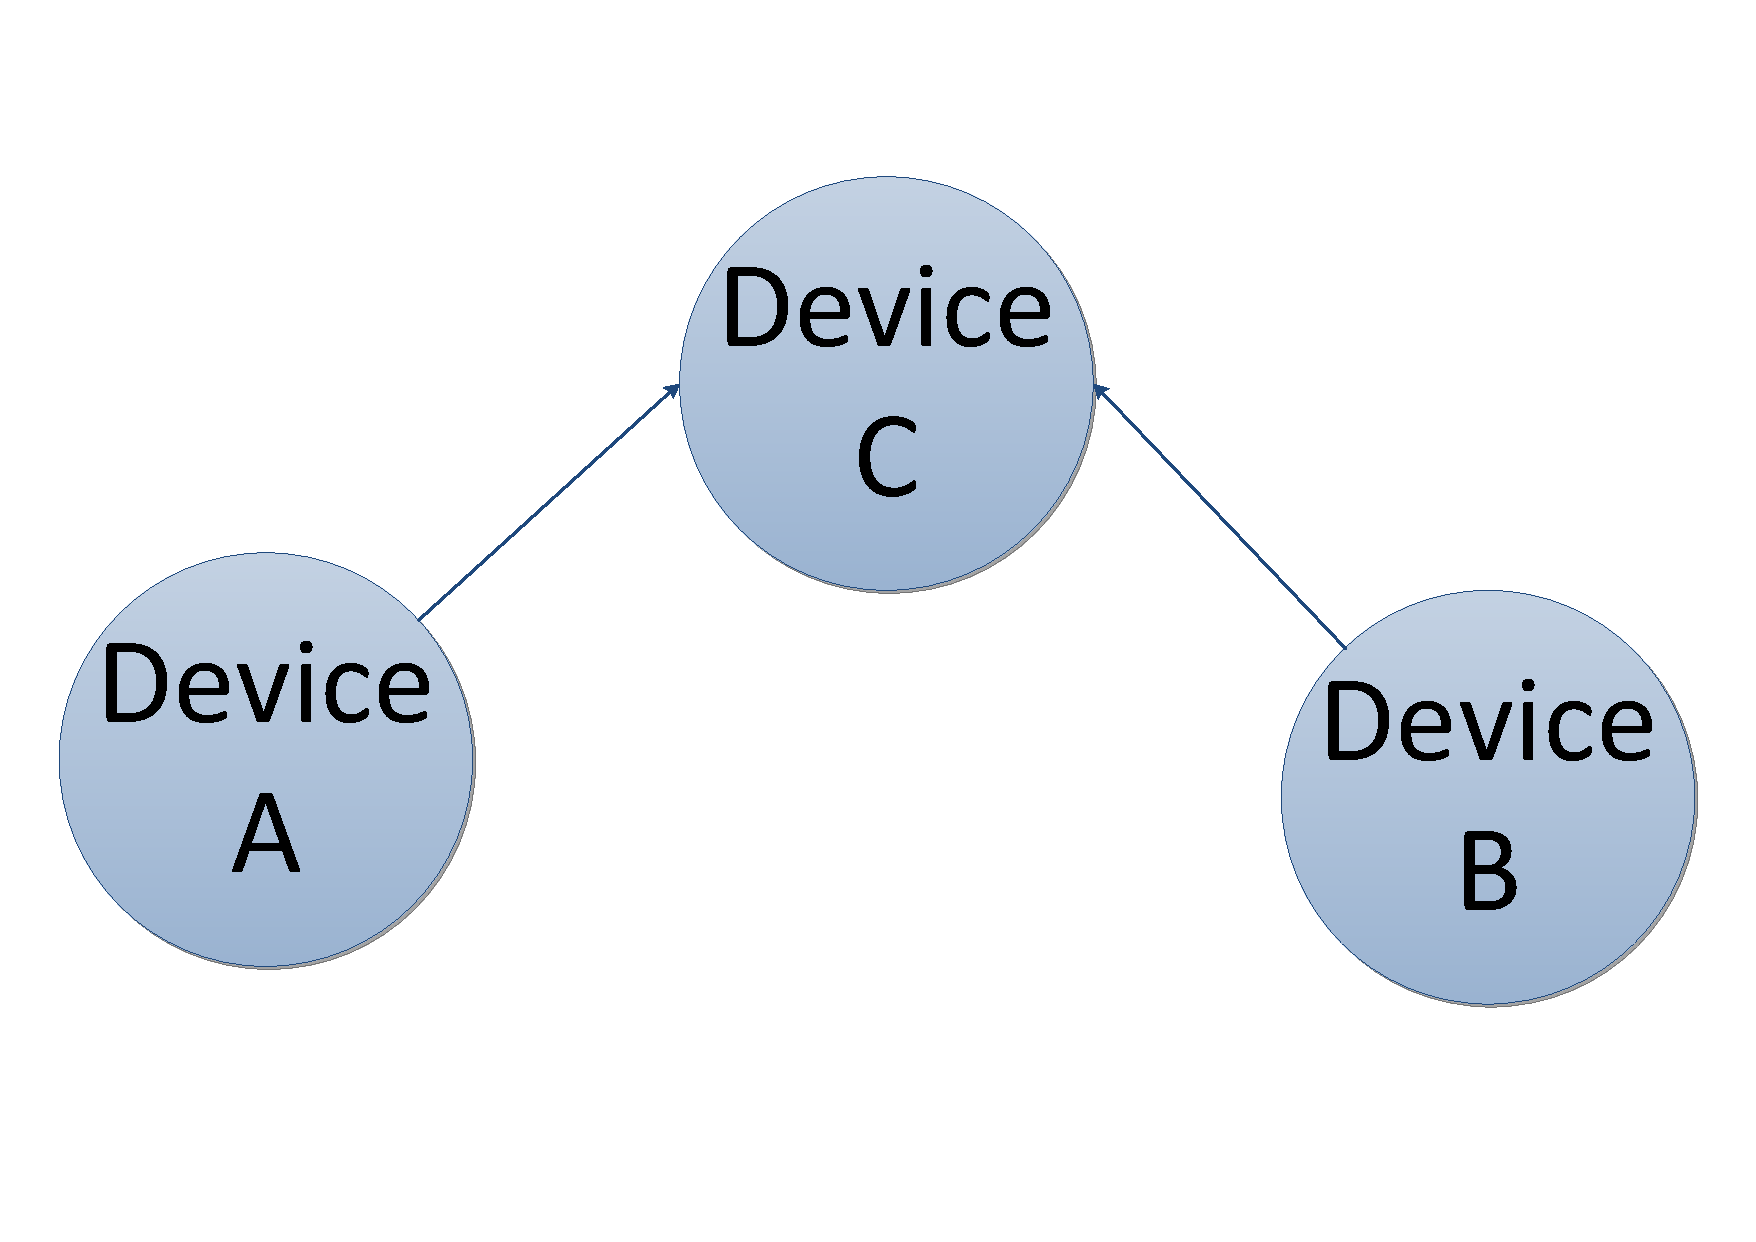
\includegraphics[width=3in]{images/relatedWork/TDMAScheduleAndHiddenNode.pdf}
	\caption{Device A and device B can both communicate with device C, but A and B are out of range of each other.}
	\label{fig:images_relatedWork_hiddenNodeProblem}
\end{figure}


\section{MAC Layer Protocols}

% What is a mac-layer protocol 
Carrier sense multiple access (CSMA)~\cite{generalCSMA, generalCSMAPart2} is a general protocol that is general to networking 
devices that have a shared channel. 
Designed by Kleinrock and Tobagi in 1975 for transmitting data over radio, CSMA requires devices to listen on the channel
to ensure no other devices are transmitting before beginning a transmission. The `carrier sense' part of the name comes from 
the device that is ready to send checking (or sensing) to see if there is already a transmission in progress. 
Since the protocol is designed to have many devices sharing the same channel, it is a 
`multiple access' protocol. CSMA has a problem called `the hidden node problem'. This arises when two 
devices that are out of radio range of each other are communicating with the same device that is in 
between the two. This problem can be seen in Figure~\ref{fig:images_relatedWork_hiddenNodeProblem}, where device A and B 
are both trying to communicate with device C. Device A and B do channel checks and do not hear any noise on the channel,
so they begin transmitting. Device C gets both transmissions at the same time, causing a collision in the messages, and 
neither of the messages are received.



%\begin{figure}[htbp]
\begin{figure}[htb]
	\centering
		
\includegraphics[width=2.5in]{images/relatedWork/CSMA.pdf}
	\caption{A CSMA handshake between two devices.}
	\label{fig:images_relatedWork_CSMA}
\end{figure}

CSMA has been adapted to WSNs by Woo and Culler~\cite{CSMA}, adding some enhancements to make 
transmissions more reliable. Woo and Culler added the idea of a two-way handshake to transmit 
messages across the network. The device sends a `ready to send' (RTS) message 
to the intended recipient (which is heard by all surrounding devices due to the shared medium). If the intended
recipient is not currently busy, it sends back a `clear to send' (CTS) message. CSMA handshaking is illustrated in  
Figure~\ref{fig:images_relatedWork_CSMA}. Woo and Culler also show that in WSNs that are largely collision-free, the ACK
step of the handshake can be dropped for energy savings. CSMA remains a major part of most WSN communication
due to its simplicity and effectiveness in detecting collisions.



\begin{figure}[bth]
	\centering
		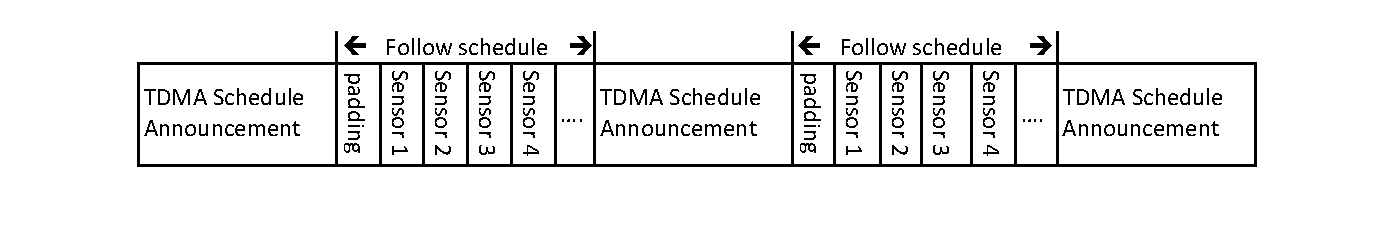
\includegraphics[width=5.5in]{images/relatedWork/tdmaSchedule.pdf}
	\caption{A sample of a TDMA schedule}
	\label{fig:images_relatedWork_tdmaSchedulev003}
\end{figure}

Time division multiple access (TDMA)~\cite{TDMA} is another method for allowing multiple 
devices to share a radio channel. Since the channel is shared, only one device can successfully
transmit at a time. If more than one device is transmitting at the same time, the messages
will collide, and neither message will be received correctly. To avoid having two devices
transmitting at the same time, a coordinator device announces a schedule that defines when and how long
the devices in the immediate area are allowed to transmit.
A visual representation of TDMA can be seen in Figure~\ref{fig:images_relatedWork_tdmaSchedulev003}.


%\section{Proactive and Reactive Networks}
%\textbf{Be nice to talk about this} Leach is reactive, teen? is reactive (like a fire alarm)


\section{Non-clustering Protocols}

Sparse Topology and Energy Management (STEM), designed by Schurgers et al.~\cite{stem} is a simple MAC protocol that uses peer to peer messaging without a clusterhead to 
send messages across a network. 
Since having the radio on drains the battery quickly, all motes cycle between listening and sleeping to conserve energy. The motes do not synchronize 
the schedule for sleeping and listening times, so motes poll neighbouring motes to send messages 
across the network. Polling wastes transmissions, since a mote will continue to send messages to a mote that is asleep until the 
mote wakes up and responds to the polling. No synchronization means that energy is wasted sending 
messages that are not received by anything.

% Directed Diffusion 
Created by Intanagonwiwat et al.~\cite{directedDiffusion, nextCentury}, Directed Diffusion 
uses peer-to-peer communication to transmit messages across the network. Directed Diffusion 
does not use clusterheads or coordinator devices to collect or route information. Since 
there are no clusterheads, all the devices in the network are tasked with 
tracking where the sink is in the network, and then transmit messages to devices in the direction
that the sink is. Intanagonwiwat et al.\ use a type of beaconing as a simple routing protocol. The
sink announces its position periodically to its neighbouring nodes. The neighbouring nodes then announce
to their neighbours that they are one hop away from the sink. This pattern continues until the entire network
knows how many hops away from the sink they are.  Directed Diffusion provides effective routing 
information with low overhead. Intanagonwiwat et al.\  considered sending some extra information with the beacons,
such as which sinks are interested in what information being sensed, but did not consider sending 
extra information about the motes along with the beacon.

% Gossiping
Gossiping is a simple way of 
increasing the chances that a message will be received at the sink. Hedetniemi et al.~\cite{gossiping} discussed
the simplicity and simple gains achieved by using gossiping in their survey paper on gossiping.
Gossiping, in general, is sending the same message along multiple routes 
to the sink. In a network with packet loss, sending multiple copies of the same message will increase the odds 
the message will be received at the sink. This also has the side-effect of possibly having the same message received at the 
sink multiple times. Another negative side-effect is that more transmissions, and therefore more power is needed to 
send one message to the sink. Though an effective way of sending messages, the cost involved in sending the messages
must be considered before using a gossiping technique.

% flooding
To quickly disseminate data, flooding~\cite{wsnSurvey} can be employed to broadcast a message across an entire WSN.
Flooding can be considered the extreme case of gossiping, where a message is announced to all surrounding 
devices, which in turn announce the same message. This is a good method for sharing routing information
quickly, but is expensive. All the devices in the network must be on, and will receive and transmit the message.
Flooding also tends to cause many collisions in the network, as all the devices will repeat the message shortly after 
receiving the message.


% smac ~\cite{smac}
S-MAC~\cite{smac} is a reliable way of moving data across a WSN without using clusterheads.
Ye et\. al outline the important features of a successful MAC layer protocol: energy efficiency, 
fairness (all motes have an equal chance of messages reaching the sink), low message latency and high throughput. 
Due to the constrained nature of WSNs, it is difficult or impossible to have all of these features, though 
networks can be tuned to enhance the desired features the network should have. An example of this 
is that a network could have better throughput, but lowered energy efficiency. S-MAC does sleep
cycling to improve the lifespan of the network, with periodic listening states to check
if any devices are trying to send to it. To avoid polling, S-MAC uses synchronization 
techniques to wake all the devices at approximately the same time, so no devices will be polling 
a device that is sleeping.




% Pegasis
Power Efficient Gathering in Sensor Information Systems (PEGASIS), designed by Lindsey and Raghavendra~\cite{pegasis},
uses global knowledge of the network to create
paths to the sink. PEGASIS saves energy by using greedy algorithms 
to create a near-optimal path to the sink. Motes hop
messages to neighbours that are closer to the sink. When a mote
receives a message, it performs message fusion on the message, then sends
the fused messages to a neighbour that is closer to the sink. Motes
using PEGASIS accept many messages and send one message per round due to this data fusion and 
hopping setup. Reducing the number of messages sent reduces the amount of energy used 
while the network runs.
PEGASIS' use of global knowledge is unrealistic in most network deployments (e.g. WSN nodes launched from a plane,
thrown into a bush) and therefore limited in its real-world applications.


\section{Clustering Protocols and Communication}

The standard approach for clustering, designed by Heinzelman et 
al.~\cite{leach}, is Low-Energy Adaptive Clustering Hierarchy (LEACH). LEACH 
is a commonly used algorithm for clustering and low energy communication. Most 
other clustering algorithms are in some way extensions of LEACH.  
Being the earliest clustering protocol for WSNs, LEACH uses somewhat 
simplistic methods for electing clusterheads. This simplicity is actually the key strength 
of LEACH, since the clusterhead election makes no assumptions about the 
network.  Heinzelman et al.\ did not consider heterogeneity or mote 
capabilities for LEACH.

Some protocols focus on sensing and reporting anomalies. Anomalies sensed
could be fires, earthquakes, security alerts, etc. Threshold sensitive Energy Efficient 
sensor Network (TEEN)~\cite{teen}, developed by Manjeshar and Agrawal, focuses on 
only reporting anomalies that are worth reporting, not wasting transmissions
on data that is not of interest. Since staying on and transmitting messages uses 
the most energy in WSNs, TEEN only sends messages if the sensor readings are
important enough to send. TEEN uses a threshold to define whether or not a
sensor reading is valuable and worth sending to the sink or not.
TEEN is a reactive-style WSN, it is not designed to regularly send information to the
sink, only if an anomaly that is being monitored occurs will a 
message be sent to the sink. This is useful for monitoring for fires or 
intruders and the like, but not useful for monitoring a resource over time.


Soro and Heinzelman~\cite{coveragepreservation} reported that, when only using 
residual energy in a mote for electing a clusterhead, the lifespan of the 
network is negatively affected when compared to using more than one factor. 
This demonstrated that the benefits of using hybrid criteria when choosing a 
clusterhead outweigh the overhead it generates. While Soro and Heinzelman showed that 
comparing more than one factor between motes in an election generates 
excessive overhead, they did not consider summarizing multiple factors into 
one hybrid criteria.

SPIN, designed by Kulik et al.~\cite{spin} uses an advertisement phase
where a mote informs surrounding motes about the message that it has. The surrounding
motes then can request the message from the mote that sent the advertisement. 
There is metadata in the advertisement that has some details about the message
that can be requested. This advertisement phase is interesting in that
any metadata could be in the advertisement message, such as information
about the mote, or messages to surrounding motes. Kulik et al.\ only considered 
sending information about the message that is ready to be sent.

Building on the foundation of LEACH, Younis and Fahmy~\cite{heed}  created 
Hybrid Energy-Efficient Distributed clustering (HEED) to address the issue of 
selecting better clusterheads. HEED uses a hierarchy much like LEACH, but uses 
more intelligence to choose the next clusterhead.  HEED uses residual power 
and a secondary parameter to create a single value describing how  well suited 
the mote is to being a clusterhead. HEED has addressed selecting better 
clusterheads based on certain parameters, but only in homogeneous networks.

Dong and Liu~\cite{resilient} created a model that chooses clusterheads based 
not only on a mote's capacity to be a clusterhead, but on data it has 
collected while the network has been alive.  If a mote had previously been 
chosen as a clusterhead, but did not do well, that mote goes to a blacklist 
and will only be chosen again if there are no known candidates to 
be a clusterhead. This use of historical data allows the network to improve 
its clusterheads over time, creating a network of clusterheads that are known 
to work well. Though Dong and Liu used knowledge of motes in the network to 
improve network lifespan, they did not consider heterogeneous networks where 
motes may have special features, such as solar panels, that could restore a 
mote with dead batteries to a useful state.

%\section{Things I'll probably delete}
%Brzozowski et al.~\cite{datareplication} investigated creating a long-term 
%data storage in long-lived WSNs.  They used data replication to ensure that 
%data is not lost during long periods when the sink is unavailable. 
%  However, Brzozowski et al.\ did not look at using heterogeneous networks 
%where some motes may have, for example, larger flash storage.
  

\section{Heterogeneous Wireless Sensor Networks}

Ou et al.~\cite{powerawareoverlay}  extended the lifespan of a heterogeneous 
WSN by making the network power-aware. Motes with larger power supplies were 
assigned the task of a clusterhead, since a clusterhead  requires more energy.  
These clusterheads were distributed around the network to create a spanning 
tree.  The power supply variance was the only heterogeneous aspect of the 
experiment and clusterheads were selected manually when the network was 
deployed, not dynamically by election.

Recognizing the lack of election protocols for heterogeneous WSN,  Smaragdakis 
et al.~\cite{stableElection} created an election protocol for heterogeneous 
WSNs.  Extending LEACH, the protocol included remaining power levels as a 
weight in clusterhead elections and concluded that this weight increased 
network lifespan.  The protocol did not  consider any other heterogeneity than 
the residual power supply. 

Brzozowski et al.~\cite{completelydistributed} explored how messages should be 
stored in heterogeneous networks, with residual energy levels being the main 
focus of the heterogeneity in the network.
Brzozowski et al.\ used a novel Media Access Control  (MAC)  protocol that 
controlled where the messages were stored and how they were routed around dying 
motes.Though Brzozowski et al. looked at routing around dead motes, they did not
consider using heterogenous motes to  extend the network lifespan even further. 
Methods such as always choosing where data should be routed, or which 
motes should be clusterheads before devices start to have critically low 
energy levels.


Hu et al.~\cite{longlivedhybrid} used two different types of motes to create a 
long-lived WSN. The motes were assigned different tasks in the network, some 
for data collection and some for routing. The authors did not consider 
self-configuring the network to utilize the heterogeneity or the possibility 
of extending the idea to more than two classes of motes. 

By creating motes with differing hardware configurations, Mhatre and 
Rosenberg~\cite{comparativestudy} showed that exploiting heterogeneity in WSNs 
can reduce network costs.  
Some of the deployed motes were inexpensive, while others were quite 
expensive. The expensive motes were configured to use the less expensive motes 
for energy-intensive tasks, allowing the more expensive motes to live longer.  
The focus was on the cost savings of a heterogeneous WSN, creating only a 
rudimentary election protocol largely based on LEACH.

Yarvis et al.~\cite{exploitHetero} described three different types of heterogeneity in 
heterogeneous WSNs, and suggested methods for best leveraging the individual 
types of heterogeneity.
The three types of heterogeneity identified were:
\begin{enumerate}
	\item \textbf{Computational Heterogeneity}. Motes have different amounts of processing power 
	available to them. Motes with more processing power should do tasks such as data fusion, or compressing messages.
	\item \textbf{Link Heterogeneity}. Some motes will have more powerful radios, providing 
	greater transmission range. Longer range allows messages to have fewer hops in the network,
	which decreases the latency time between the message being created and the message arriving 
	at its destination.
	\item \textbf{Energy Heterogeneity}. Motes have varying amounts of energy available for their use. Some motes might
	be powered externally, often called `line' or `wall' power, while other motes might have very limited
	amounts of nonrenewable battery power. Motes with more battery power should take on power-intensive tasks, 
	such as being clusterhead or performing data fusion.
\end{enumerate}
Yarvis et al.\ focused their efforts on ways of creating optimal placement of motes
with the knowledge of the heterogeneous motes in the network, and worked with S-MAC~\cite{smac} as a base
MAC protocol. They did not consider cluster-based WSNs as a way of further increasing the 
lifespan of the network.



\chapter{HCCP: Heterogeneous Clustering and Control Protocol}
\label{ch:HCCP_intro}

HCCP 
is a method for describing and advertising  the internal resources of wireless 
sensor motes, and using the strengths of the motes to increase message throughput
or extend the lifespan of 
the network. Once motes are aware of their internal resources, they should 
choose clusterheads based on the resources available. For 
example, motes that are assigned the clusterhead role use more energy. 
Therefore, motes that have extra batteries should be chosen as a clusterhead 
before motes without extra batteries. 

\begin{figure}[t]
	\centering
		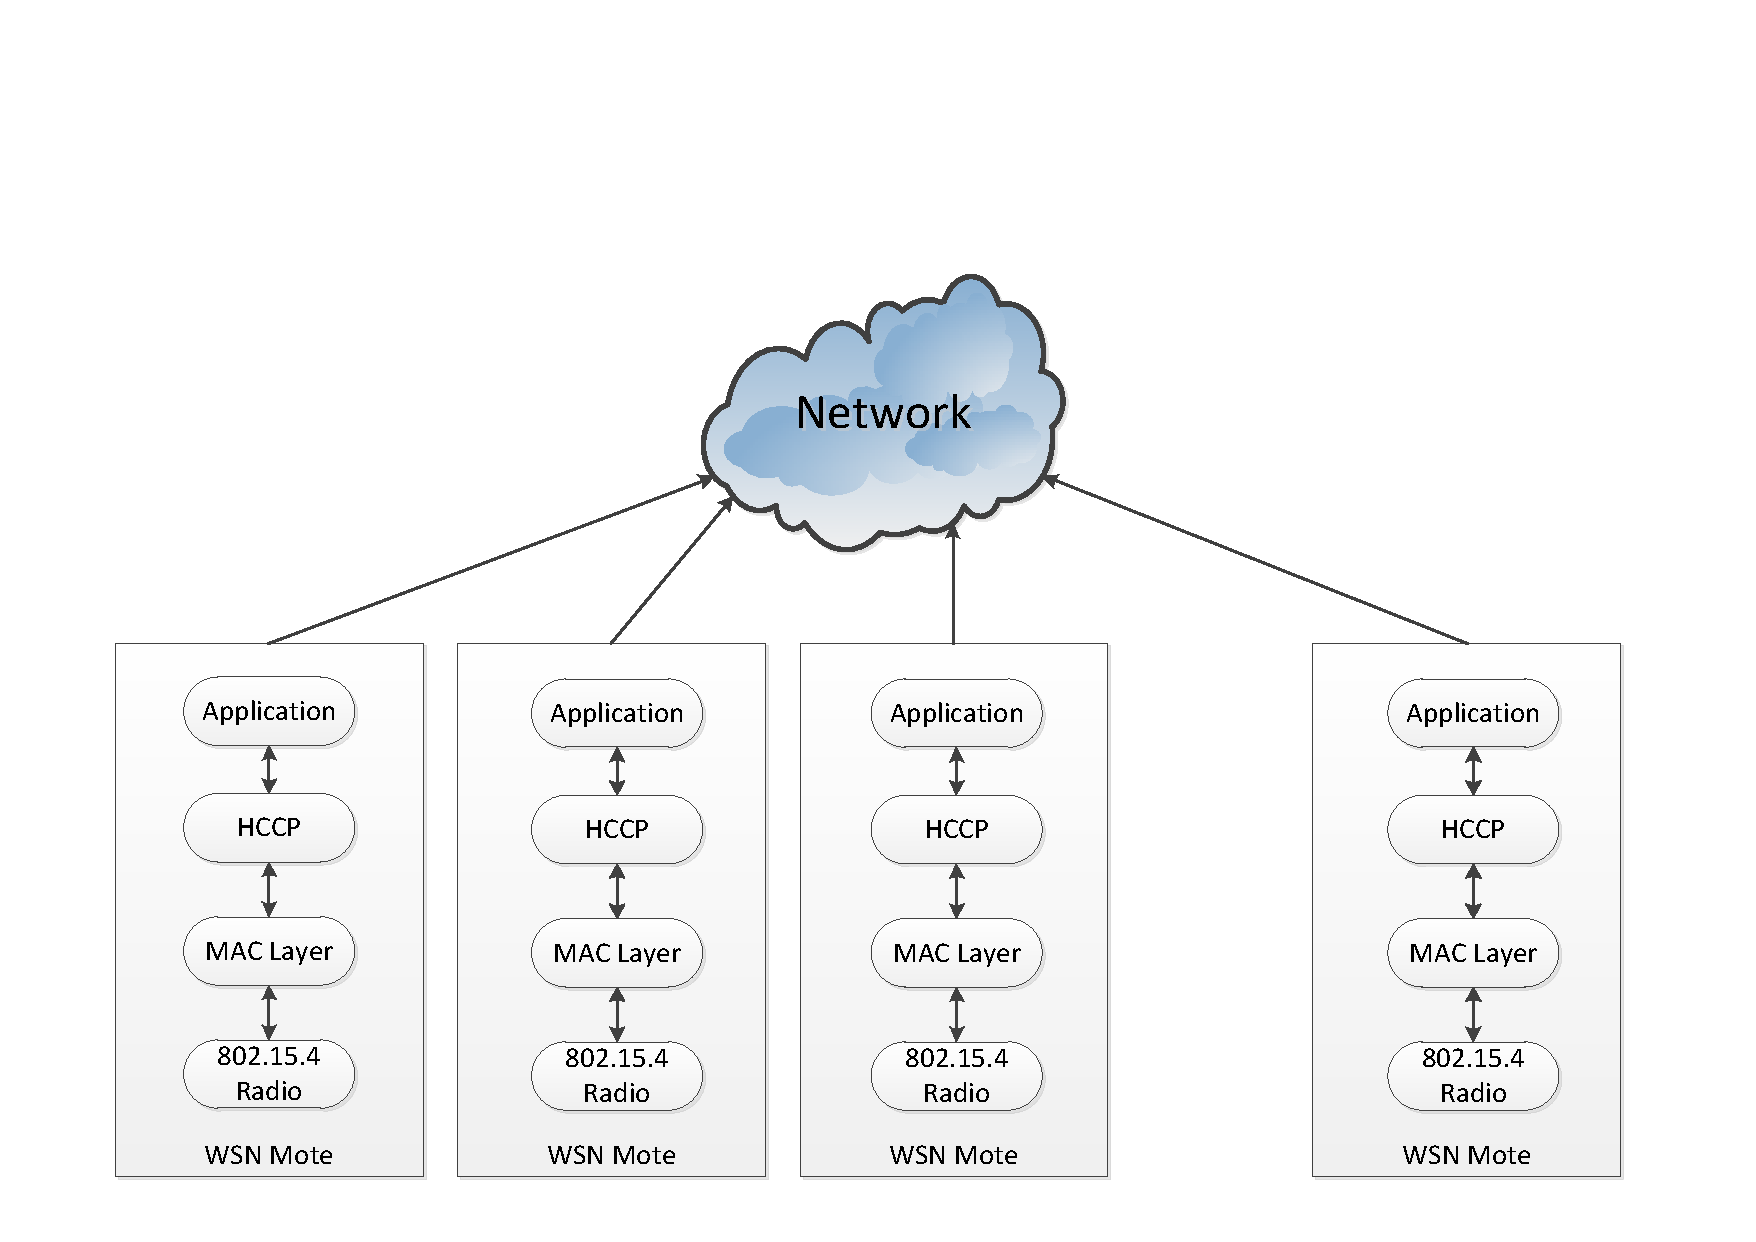
\includegraphics[width=\textwidth]{images/protocol/HCCPAsMiddleWare.pdf}
	\caption{HCCP uses existing MAC protocols and can be used by any application, acting as middleware.}
	\label{fig:images_protocol_HCCPAsMiddleWare}
\end{figure}

A mote should not only be aware of its resources, but it should also be aware 
of the requirements of the network. This is a consideration because the topology 
of WSNs are prone to change due to the battery-powered nature of its 
components (e.g., a mote with a dead battery will change the topology of the 
WSN).  Also, motes may move in the network (by some external force such as a 
person moving the mote), further changing the topology of the network.  To 
handle this unpredictability, the motes need to be aware of the motes nearby, 
but not waste excessive energy discovering them.  

HCCP acts as middleware between the MAC layer and the application layer of the 
mote, as shown in Figure~\ref{fig:images_protocol_HCCPAsMiddleWare}. 
The application layer queues messages that are ready to send, HCCP takes the
messages and sends them to the sink when possible. HCCP uses existing MAC layer protocols 
such as CSMA and TDMA, so HCCP itself is not a MAC protocol.


\section{Theory of Operation}
\label{sec:theory}

HCCP has roots in LEACH, following the design of clusterhead elections, but extends the design of LEACH 
in multiple ways. While LEACH has relatively simple clusterhead elections, where nodes
elect themselves based on a probability, HCCP has a more elaborate election process. HCCP's election 
process weighs the `goodness' of the node to be a clusterhead, and automatically limits the number of other nodes that 
will be clusterheads. HCCP has also adopted the way a LEACH network cycles between clusterhead
elections and node runtime.

The LEACH run cycle is quite simple in it's operation, and provided inspiration for the HCCP
run cycle. The LEACH network cycle is as follows:

\begin{figure}[htbp]
	\centering
		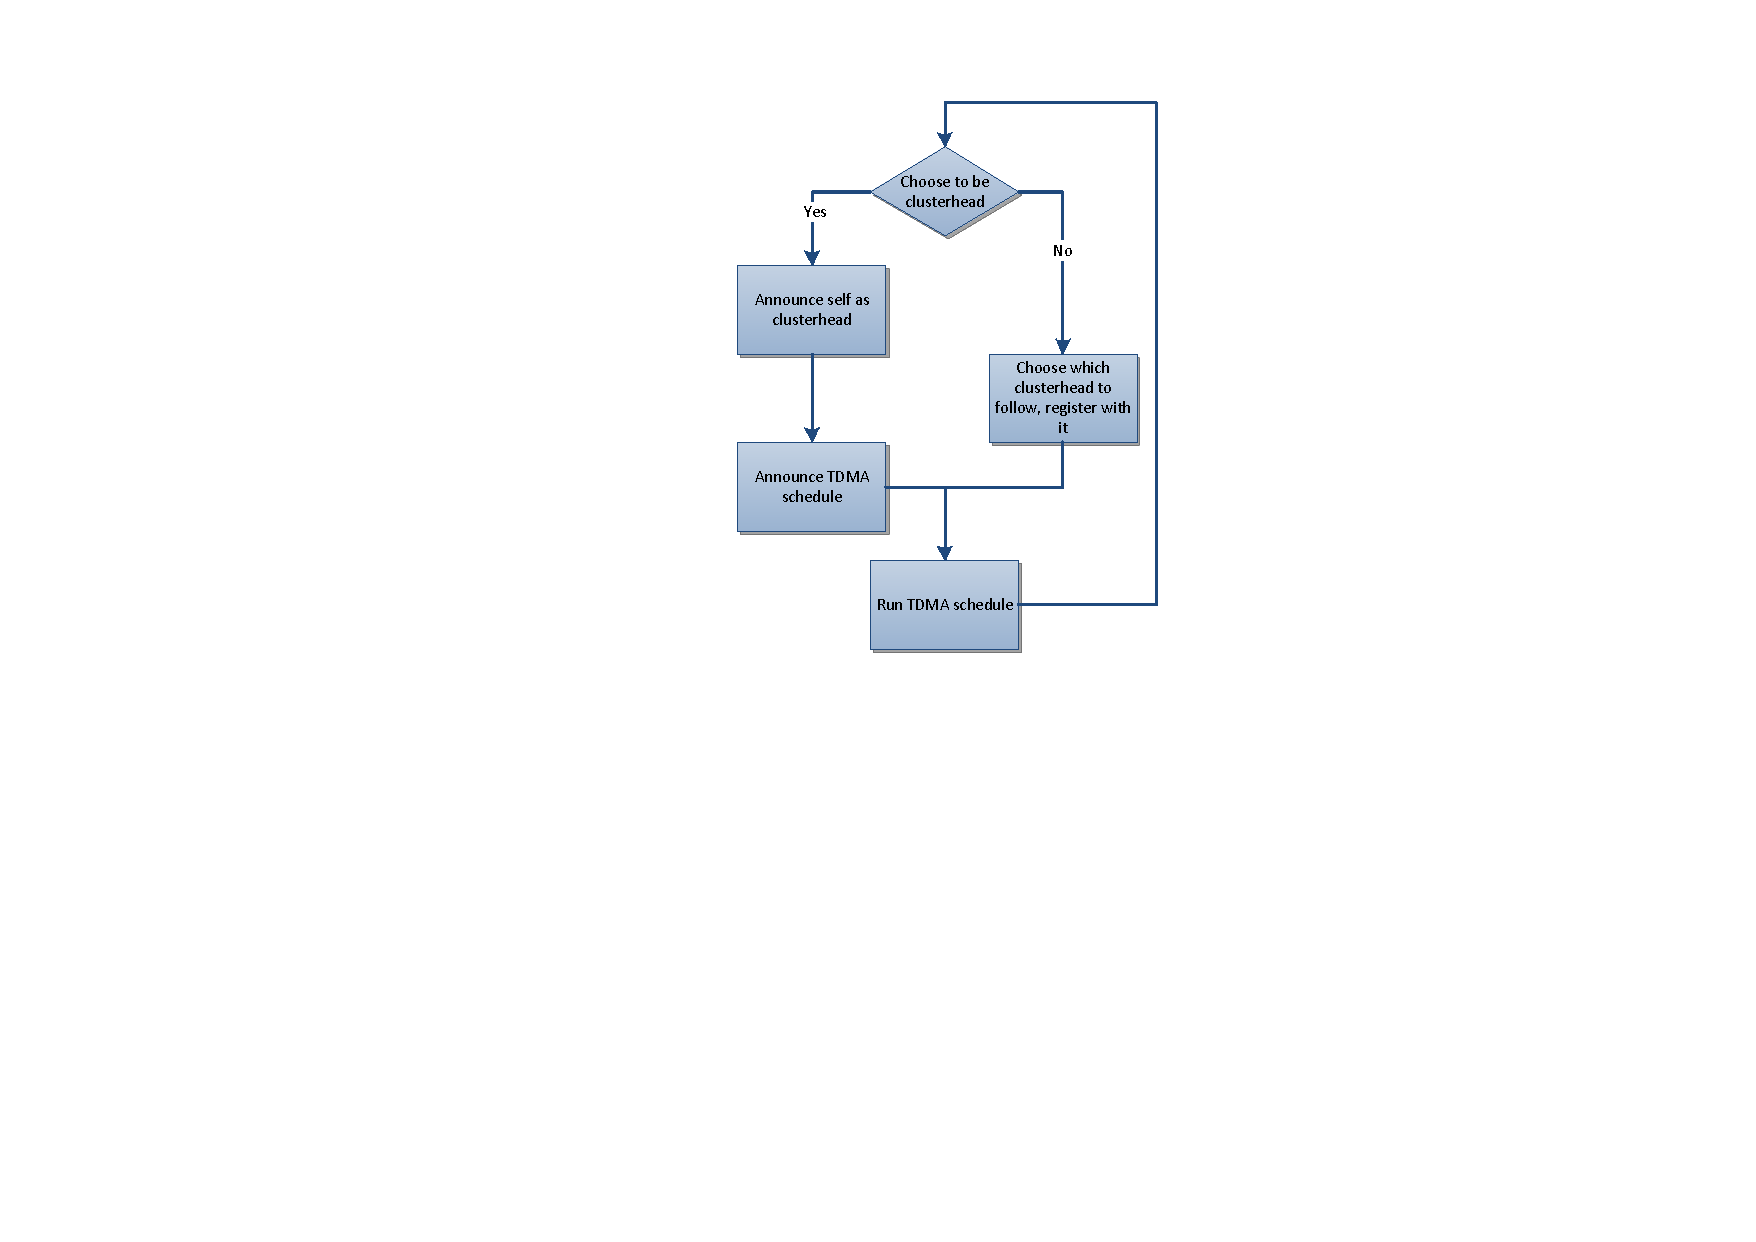
\includegraphics[height=4.2in]{images/protocol/LeachFlowchart.pdf}
	\caption{LEACH election run cycle.}
	\label{fig:leachelec}
\end{figure}

\begin{enumerate}
	\item \textbf{Clusterhead election} --- Motes choose whether not not to advertise themselves as
	clusterheads. The decision to be clusterhead is based on a how long it has been since it was a 
	clusterhead and some added randomness.
	\item \textbf{Choose cluster} --- Motes that are not clusterheads send messages to the
	clusterhead they will follow this round.
	\item \textbf{Announce Schedule} --- Clusterhead sends a TDMA % TDMA defined eariler
	schedule via broadcast. 
	\item \textbf{Cluster Runtime} --- The motes in the cluster follow the TDMA schedule, 
	taking turns sending messages to the clusterhead.
	\item \textbf{Repeat} --- Go back to clusterhead election. There can be a sleep time here to extend the network life.
\end{enumerate}


THE LEACH network cycle can be seen graphically on Figure~\ref{fig:leachelec}. The cycle is repeated until all the 
motes in the network cease to function. LEACH was focused 
on simplicity, which makes LEACH quite robust as it runs. Since every mote takes becomes a clusterhead
occasionally, there is no single point of failure -- the network will continue to function even
if a number of motes cease to function. LEACH makes a solid foundation to build upon, using the 
lessons learned from its success and building on its weaknesses.


HCCP takes the strengths LEACH, using the simplicity of the election and run cycles, adding
the ability to leverage the heterogeneity that is inherent in all WSNs. The HCCP network cycle 
is as follows and is illustrated  in Figure~\ref{fig:images_protocol_ElectionFlowchart}.


\begin{enumerate}
	\item \textbf{Clusterhead Election}
	\begin{enumerate}
		\item \textbf{Announce Candidacy} --- Announce the mote's intentions to be clusterhead. 
		Using a Goodness assessment, announce first if the mote has a good assessment.
		\item \textbf{Announce Clusterhead} - Successful candidates announce they are clusterheads.
	\end{enumerate}
	\item \textbf{Choose Cluster} --- Same as LEACH.
	\item \textbf{Announce Schedule} --- Same as LEACH. 
	\item \textbf{Cluster Runtime} --- Same as LEACH.
	\item \textbf{Roundtable Discussion} --- Any queries or announcements can be made at this time. 
	Clusterheads can opt-out, forcing a clusterhead election.
	\item \textbf{Repeat} --- Go back to Cluster Runtime for multiple iterations. Every $n^{th}$ iteration 
	(where $n$ is selected before network deployment and well-known to the network) go back to Clusterhead election.
	
\end{enumerate}

\begin{figure}[ht]
	\centering
		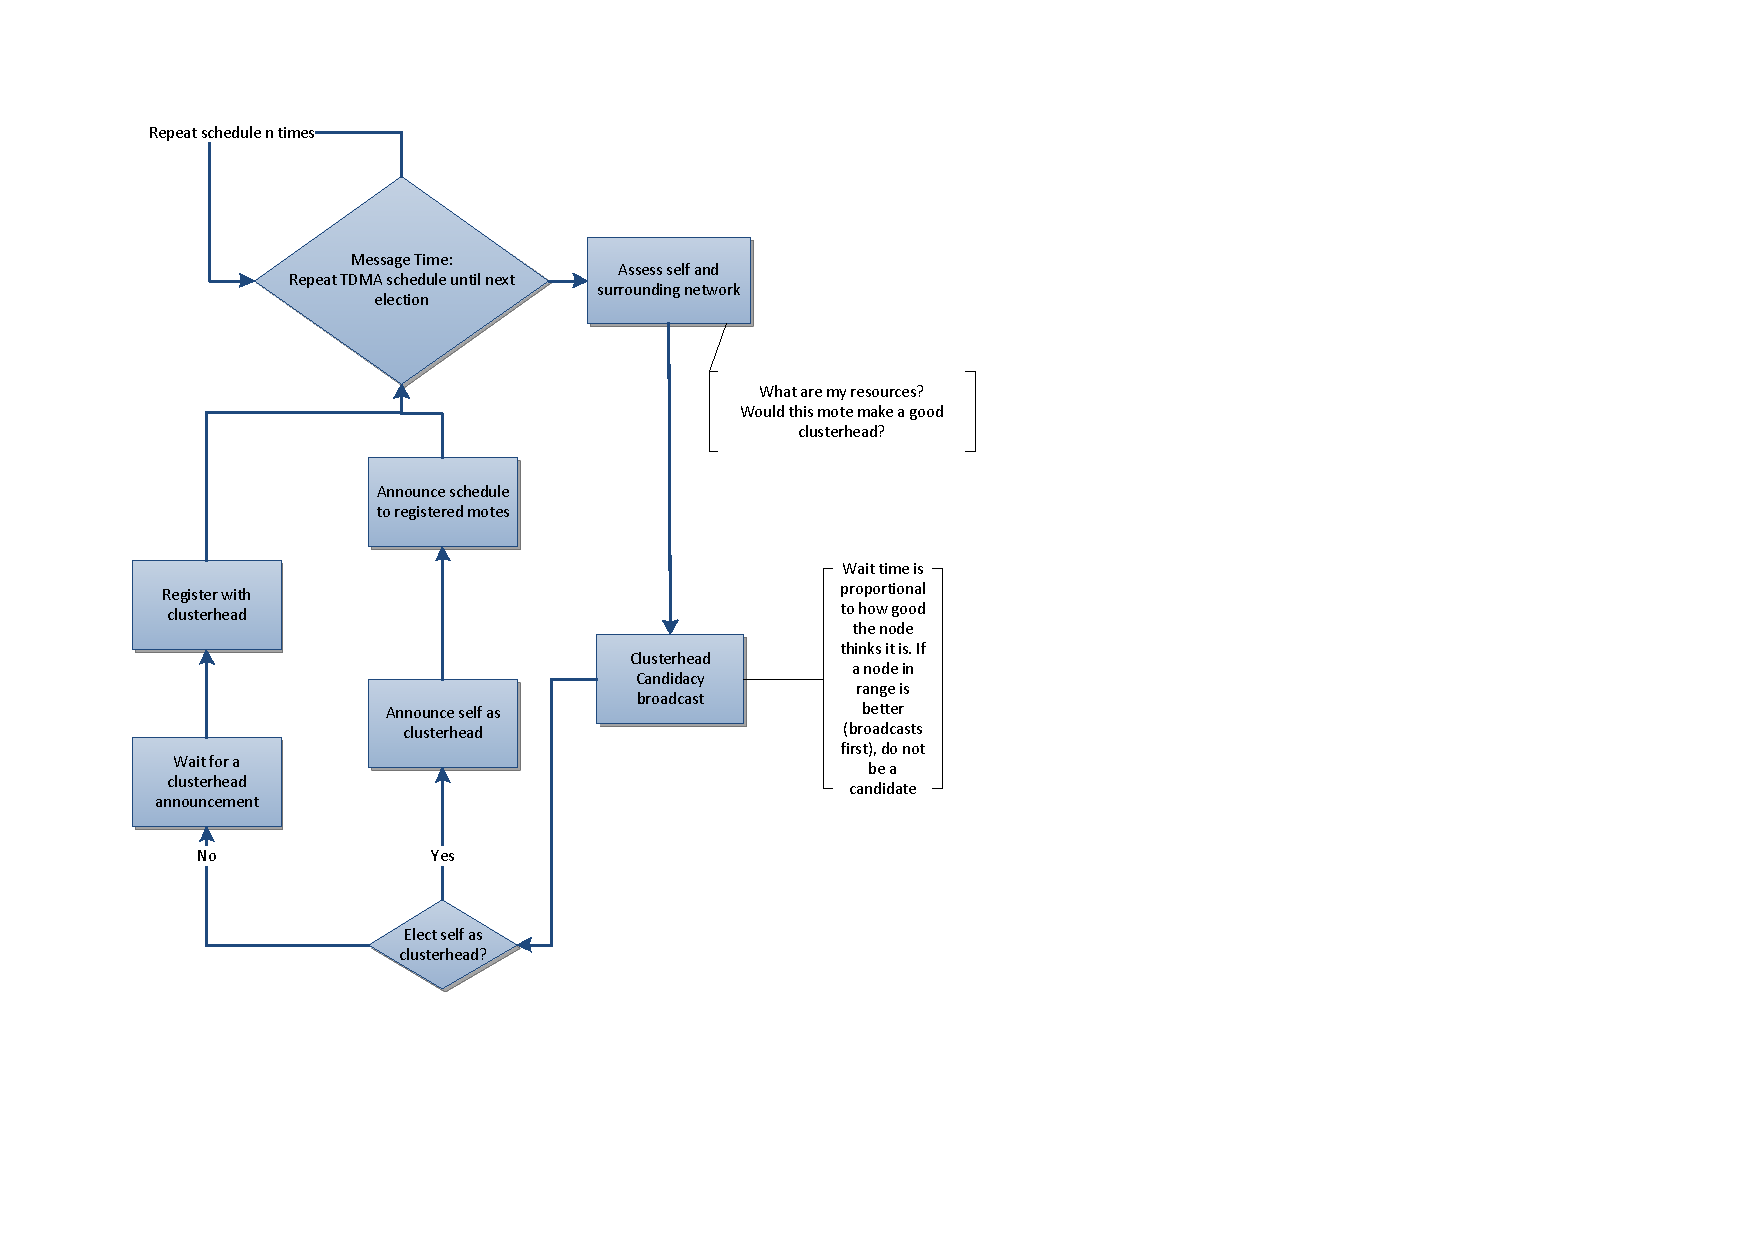
\includegraphics[height=5.75in]{images/protocol/ElectionFlowchart.pdf}
	\caption{A visualization of the HCCP election and run cycle.}
	\label{fig:images_protocol_ElectionFlowchart}
\end{figure}

HCCP uses all of the strengths of LEACH in the run cycle, further modifying the 
concept with some extra modifications that make
the network more intelligent in terms of which motes are elected clusterhead. The major additions are two-stage elections,
multiple iterations of the TDMA schedule and Roundtable Discussion (including Clusterhead opt-outs).

\subsubsection* {Two-stage election}
	Motes choose to be a clusterhead candidate before they can elect themselves clusterheads. 
	A mote determines that it would be a good clusterhead by inspecting its available resources,
	and choosing how long to wait before they announce themselves as a clusterhead.
	Motes that announce candidacy first get to be clusterheads that round.
	Motes that determine they would not be 
	very good clusterheads wait a longer time due to the Goodness Delay. If a candidacy announcement 
	from a better potential clusterhead that is relatively close in proximity 
	is overheard before a candidate broadcasts, the lesser candidate will
	not send an announcement, and demote itself to a regular cluster member.
	
\subsubsection* {Multiple iterations of schedule}
	All messages in clusterhead elections can be considered overhead, as these messages are not
	relaying any information to any destination. Further, 
	any time a mote is on without sending or receiving messages
	can also be considered overhead.
	
	To minimize time spent in clusterhead elections, they should only be run
	occasionally. LEACH runs a clusterhead election after every TDMA schedule runtime,
	which is good for distributing the burden of being a clusterhead, but creates
	lots of overhead messages. 
	
	The solution to this is relatively simple; a clusterhead election should only happen 
	occasionally. Further, a TDMA schedule does not need to be re-transmitted before
	every TDMA runtime. A TDMA schedule only needs to be transmitted after a 
	clusterhead election, which should only happen after $n$ runs of 
	the TDMA schedule. The number of times the network TDMA schedule executes ($n$) should be determined before
	network deployment. This is so it is well-known, consistent number across the entire network
	ensuring that the network does not get out of synchronization. A lower
	value of $n$ should be chosen if the network is to be adaptive and flexible, while
	a larger value of $n$ should be chosen if the network should have as little overhead as possible.

\subsubsection* {Roundtable Discussion}
	After each run of the TDMA schedule, all the motes in the network turn on 
	their radios to listen for broadcasted announcements or queries.
	This is the time where clusterheads can opt-out, synchronization messages
	can be exchanged and routing tables can be shared. The Roundtable Discussion 
	time can also be used to extend HCCP in various ways, providing a
	time to implement neighbour discovery and adjust radio power accordingly, or whatever
	the network administrator chooses.



\subsubsection* {Clusterhead opt-out}
\label{optout}
	Since the TDMA schedule published by the clusterhead will be followed 
	multiple times, the clusterhead's performance may degrade, eventually causing
	the entire cluster to perform poorly. LEACH averts this problem by running 
	a clusterhead election after every TDMA schedule runtime.
	Since HCCP runs multiple iterations of the TDMA schedule, the clusterhead needs a
	way to retire if it begins to degrade.

	A clusterhead can announce its retirement during the Roundtable Discussion. 
	When a clusterhead retires,
	it forces a small clusterhead election, with only the motes in the 
	one affected cluster acting in the clusterhead election. The network
	does a LEACH-style clusterhead election. The first mote that announces
	that it is a clusterhead becomes the new clusterhead for the cluster.
	The Goodness Delay is used to decide how long a mote will wait before
	it sends a clusterhead announcement, using the same method as candidacy announcements.
	This way, the best possible clusterhead mote should become the replacement clusterhead.


	The cluster then continues to run using the existing TDMA schedule
	for the remaining  iterations
	before the next full clusterhead election.




\section{Implementation Details}
\label{ch:implementation}

The following is a discussion of how HCCP works at an implementation level.
Since HCCP is designed to be run on different hardware, with
different capabilities, it is best to describe the network
setup in terms of communication. Specifics about mote design,
real-time operating systems and communication stacks are abstracted. 


\subsection{Clusterhead Election}


HCCP takes a different approach than LEACH to electing clusterheads.
Motes can't just be cluster members, even though being a clustermote every round
is the most energy-efficient thing to do. 
A problem inadvertently created by HCCP's attempt to allow more motes
be clustermembers, is that if a mote is by a sink, it would never choose to be a clusterhead. 
In the Clusterhead Candidacy phase, the sink will always broadcast first, never allowing
motes in range of the sink to be clusterheads, since they would always concede to the sink.
%If motes never became clustermotes due to there being a very good 
%clusterhead next to them, there would be an invisible wall around the 
%sink of motes that never become clusterheads. 
Since no motes
around the sink would ever be clusterheads,
motes out of range of the sink cannot hop messages to the sink. This would create an invisible wall around the sink, where motes past
the wall will never have messages reach the sink. If a mote does not complete any messages, it is
suffering starvation, a term taken from task scheduling in operating systems when processes will never run due
to higher priority processes continually running.
The effects of starvation can be seen in Figures~\ref{fig:images_HCCPBlocking_hccpblocking} and~\ref{fig:starvationMap}.
Figure~\ref{fig:images_HCCPBlocking_hccpblocking} shows a comparison of distance from the sink to how many messages have been 
received at the sink, and it is clear that no messages beyond 100 arbitrary distance units from the sink would ever have 
messages received at the sink.
Figure~\ref{fig:starvationMap} shows a map of where the motes are that have completed messages, and which motes are 
suffering from starvation (the sink is the green triangle in the middle of the network).
A few messages from motes beyond the invisible wall can be received at the base station if
collisions in clusterhead candidacy messages, allowing motes within the invisible wall to become clusterheads. Motes that 
did not get that message could then elect to be a clusterhead, allowing messages in 
from beyond the wall. Starvation does not happen in LEACH since the clusterhead elections happen 
independent of each other, as shown in Figure~\ref{fig:StarvationLeach} which is created from the 
same network with the same configuration settings using LEACH as an election protocol. 
Therefore, a solution is needed to avoid creating the invisible wall that 
the Clusterhead Candidacy phase has created.

\begin{figure}[htb]
	\centering
		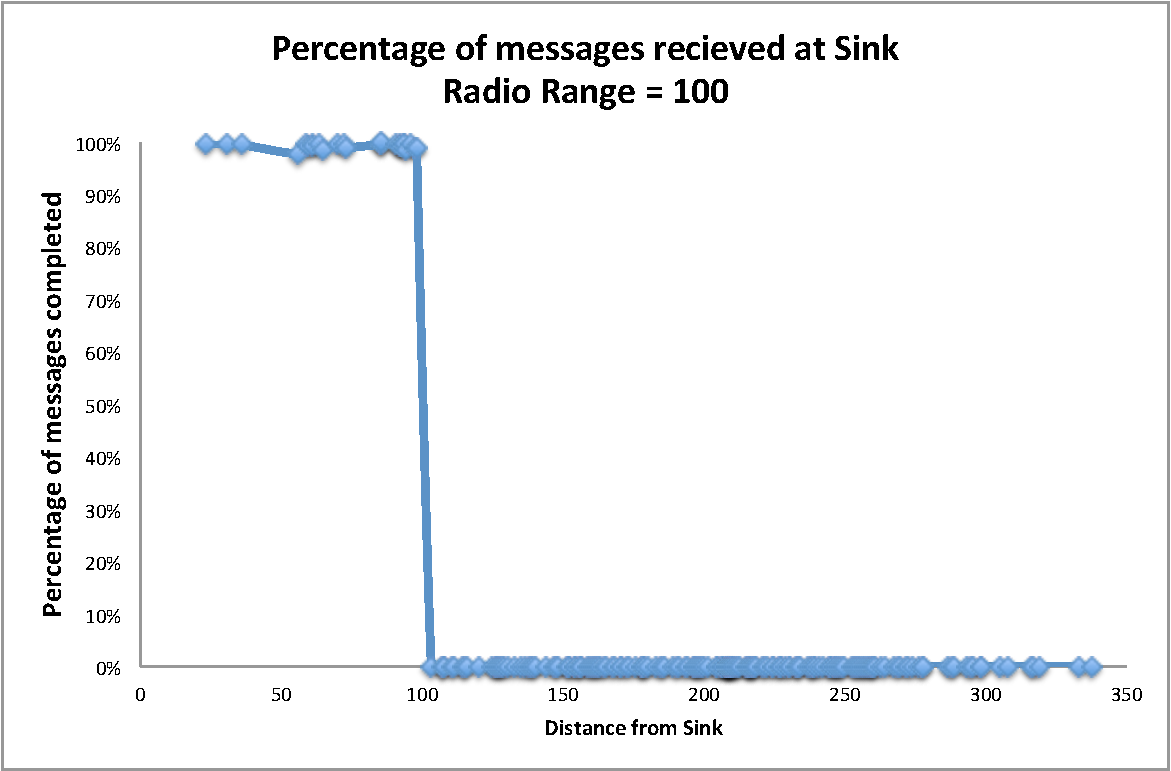
\includegraphics[height=3in]{images/HCCPBlocking/starvation.pdf}
	\caption{An invisible wall created due to HCCP clusterhead candidacy messages.}
	\label{fig:images_HCCPBlocking_hccpblocking}
\end{figure}
\begin{figure}[htb]
	\centering
		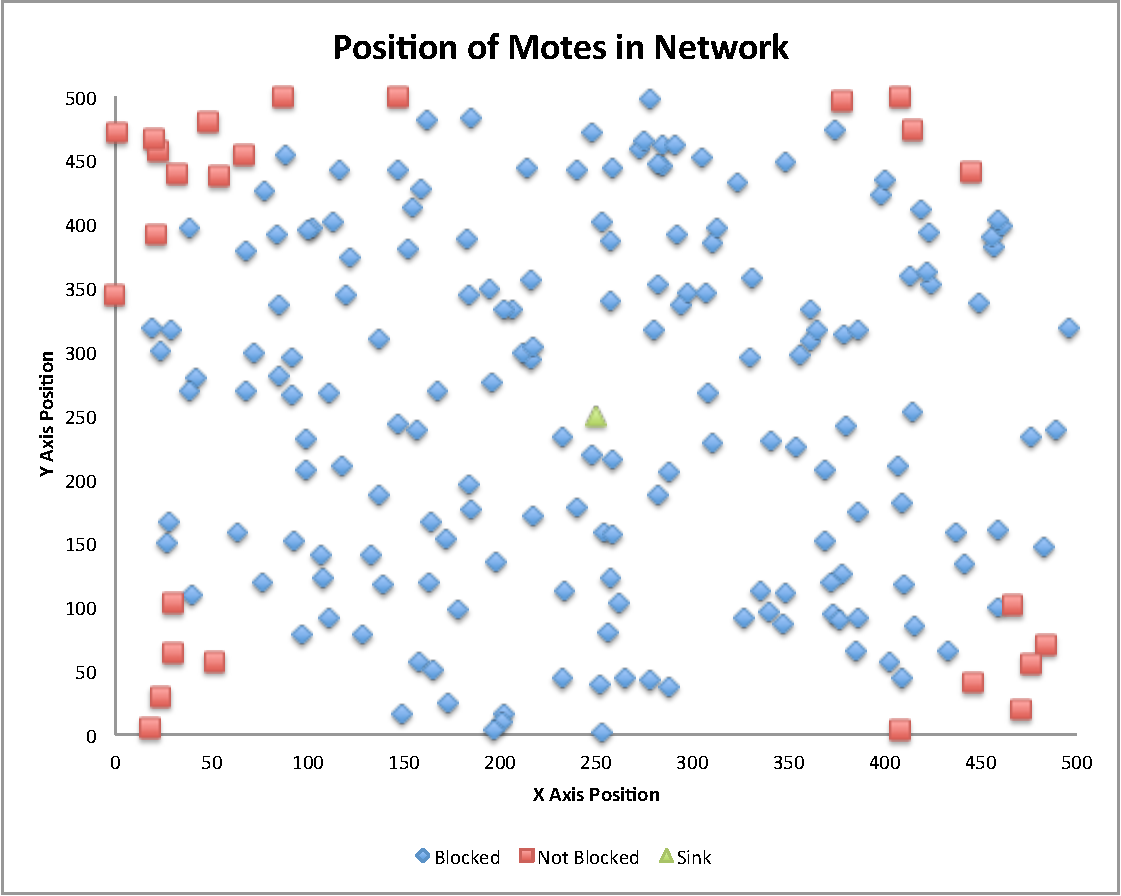
\includegraphics[height=3.5in]{images/HCCPBlocking/starvationMap.pdf}
	\caption{HCCP messages received at the base station. There is no way messages outside the radio range of the sink can send messages to the sink.}
	\label{fig:starvationMap}
\end{figure}

\begin{figure}[htb]
	\centering
		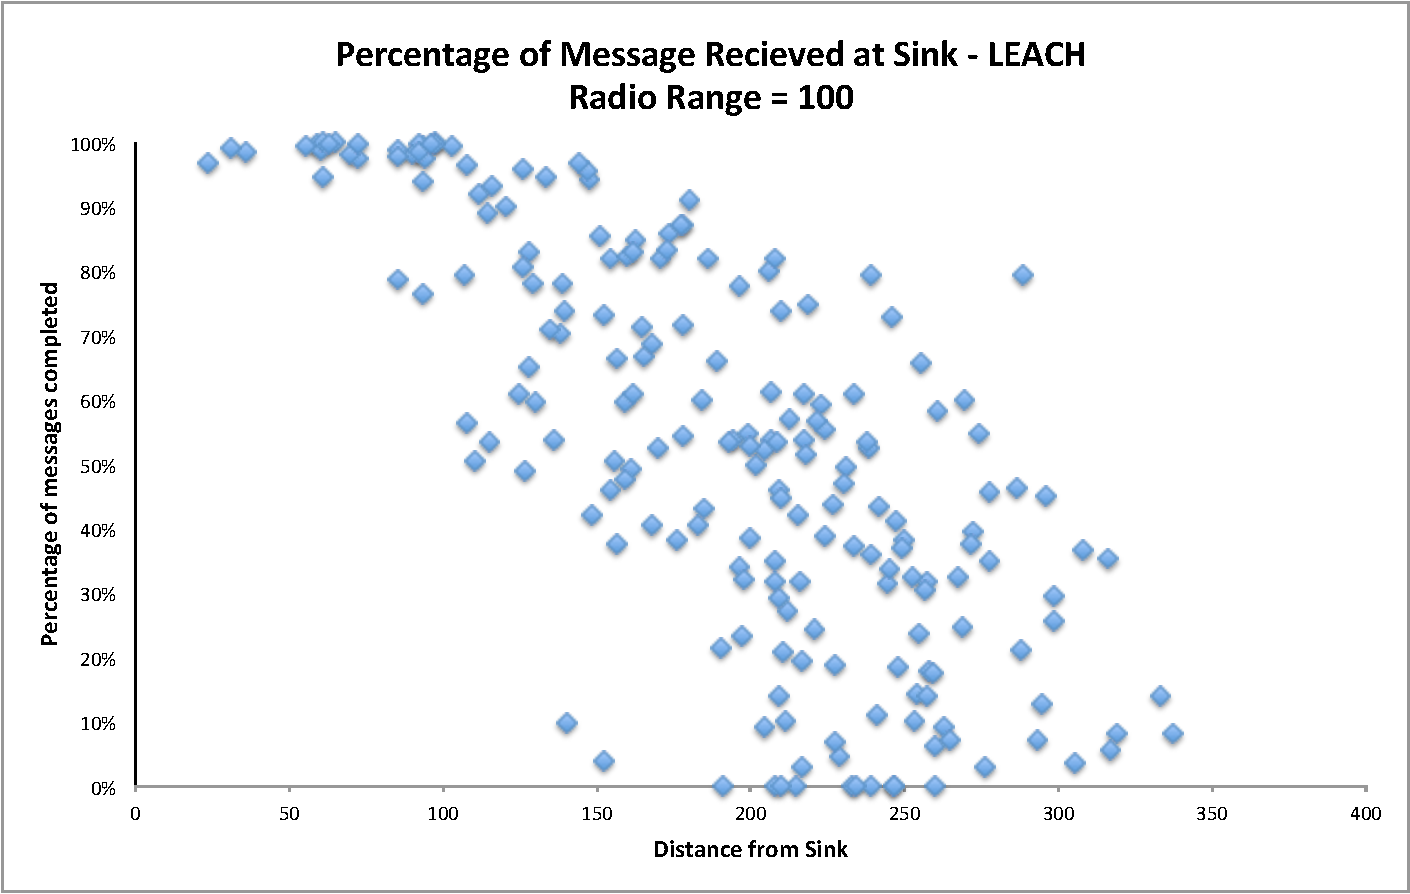
\includegraphics[height=3in]{images/HCCPBlocking/StarvationLeach.pdf}
	\caption{LEACH messages reached at the base station, note there is no `wall' blocking messages.}
	\label{fig:StarvationLeach}
\end{figure}

There are two different approaches to eliminate the problem of the `invisible wall' in HCCP.
\begin{enumerate}
\item The sink can sleep for a cycle. Since the sink would not send a
clusterhead candidacy message, the surrounding motes would then 
be able to become clusterheads. This would allow messages to flow into the 
motes in range of the sink from motes out of range of the sink.
\item Motes can choose to be clusterheads \emph{even if} there is a better clusterhead in range.
Since the sink will always be a better clusterhead than a mote, a mote should 
be able to ignore all other candidacy messages and become a clusterhead.
\end{enumerate}


Both of these have drawbacks. If the sink turns off for a cycle, the latency time for messages
will go up, since no messages will be received at the sink for this time. If clusterheads
are allowed to randomly choose to be clusterheads, there will be more collisions
due to the increased number of messages being sent during clusterhead messaging times (clusterhead
elections and the like).

To discover which of these methods is better to  use, a simulation of both LEACH and HCCP 
was created and the results were compared, and are compared later in section~\ref{sleepVSsubop}.


\subsection{HCCP Goodness Delay}
\label{subsec:goodnessDelay}
%The better I am, the sooner I announce it.

To ensure that motes that are better at being clusterheads are chosen to be clusterheads, the timing that
is inherent in an election/run WSN such as LEACH is leveraged.  If a mote has the right qualifications
for being a good clusterhead, it announces its candidacy first. If another mote that was
going to announce its clusterhead candidacy hears the a different mote's candidacy message first,
it will not be a clusterhead that round. 

The Goodness Delay is created by delaying a percentage of the available time. 
%is derived by a `percentage of goodness' 
Motes that are well suited for being a clusterhead will create a small delay (therefore
announcing itself as a potential clusterhead earlier), and motes that are not well suited for being 
a clusterhead will have longer delays.

Since the heterogeneous assessment can focus on different heterogeneous factors,
the way of determining how long to delay must be robust to the possible focuses.
To reflect this, a percentage of time to delay is put into a weighted average of
all the factors that will contribute to the delay timing.
The code looks like the following:

{\ssp \vskip 1em  \hangindent=0.5cm
\lstset{basicstyle=\footnotesize\ttfamily,language=Java}
\begin{lstlisting}
private double getGoodnessDelay()
{
  double delay = 0;

  // add up to n% of available time based on battery
  delay =  (availableTime * BATTERY_POWER_WEIGHT  * 
      (1 - battery.getPercentLeft() ) );

  // n% of available time based on mission
  // delay gets longer if this node wants to be a clustermote
  delay = delay + (availableTime * SENSOR_MISSION_WEIGHT *
       sensorMission );

  // n% on messagequeue size
  delay = delay + (availableTime * MESSAGE_QUEUE_WEIGHT * 
      ( messageQueue.size()/(double)maxQueueSize ) );

  // n% of random
  delay = delay + (availableTime * RANDOM_WEIGHT * 
      (goodnessRM.nextDouble()));

  // n% of duty cycling based on last round as CH.
  // more delay if I was just a clusterhead.
  delay = delay + (availableTime * DUTY_CYCLE_WEIGHT *  
      ( 1- Math.min(1, lastRoundAsClusterhead * chanceOfBeingCH)));

  return delay;
}
\end{lstlisting}
}


 \subsubsection{Continuous Nature of HCCP Goodness Delay}
     Since HCCP uses a Goodness Delay to advertise the heterogeneity of the network, it can be considered
     a continuous statistic. This is as opposed to the two/three/n-tier network that describes a network
     as a binary relationship between motes: a mote is a routing mote or not. HCCP takes what is known about 
     the mote, and translates that information into a continuous distribution via the Goodness Delay algorithm.
     The Goodness Delay calculates a percentage of `Goodness as clusterhead', and maps that Goodness to an amount
     of time to delay before becoming a clusterhead. Therefore, HCCP considers every mote to be a heterogeneous mote,
     even in a homogeneous network. Even in a homogeneous network, not all motes will be the same. Some motes will have 
     batteries that are drained more than others, and some will have no space in their message queue to become a clusterhead.
     This approach considers such factors.
     
     
 \subsubsection{Drawbacks to Goodness Delay}
     When a network is first deployed, all motes will have full batteries, empty message queues and 
     will generate approximately the same Goodness Delay.
     This would cause the Clusterhead Candidacy and Clusterhead Election time to effectively only be in the first 10th or so of the 
     time allotted to the stage.
     
     \begin{figure}[t]
      	\centering
      		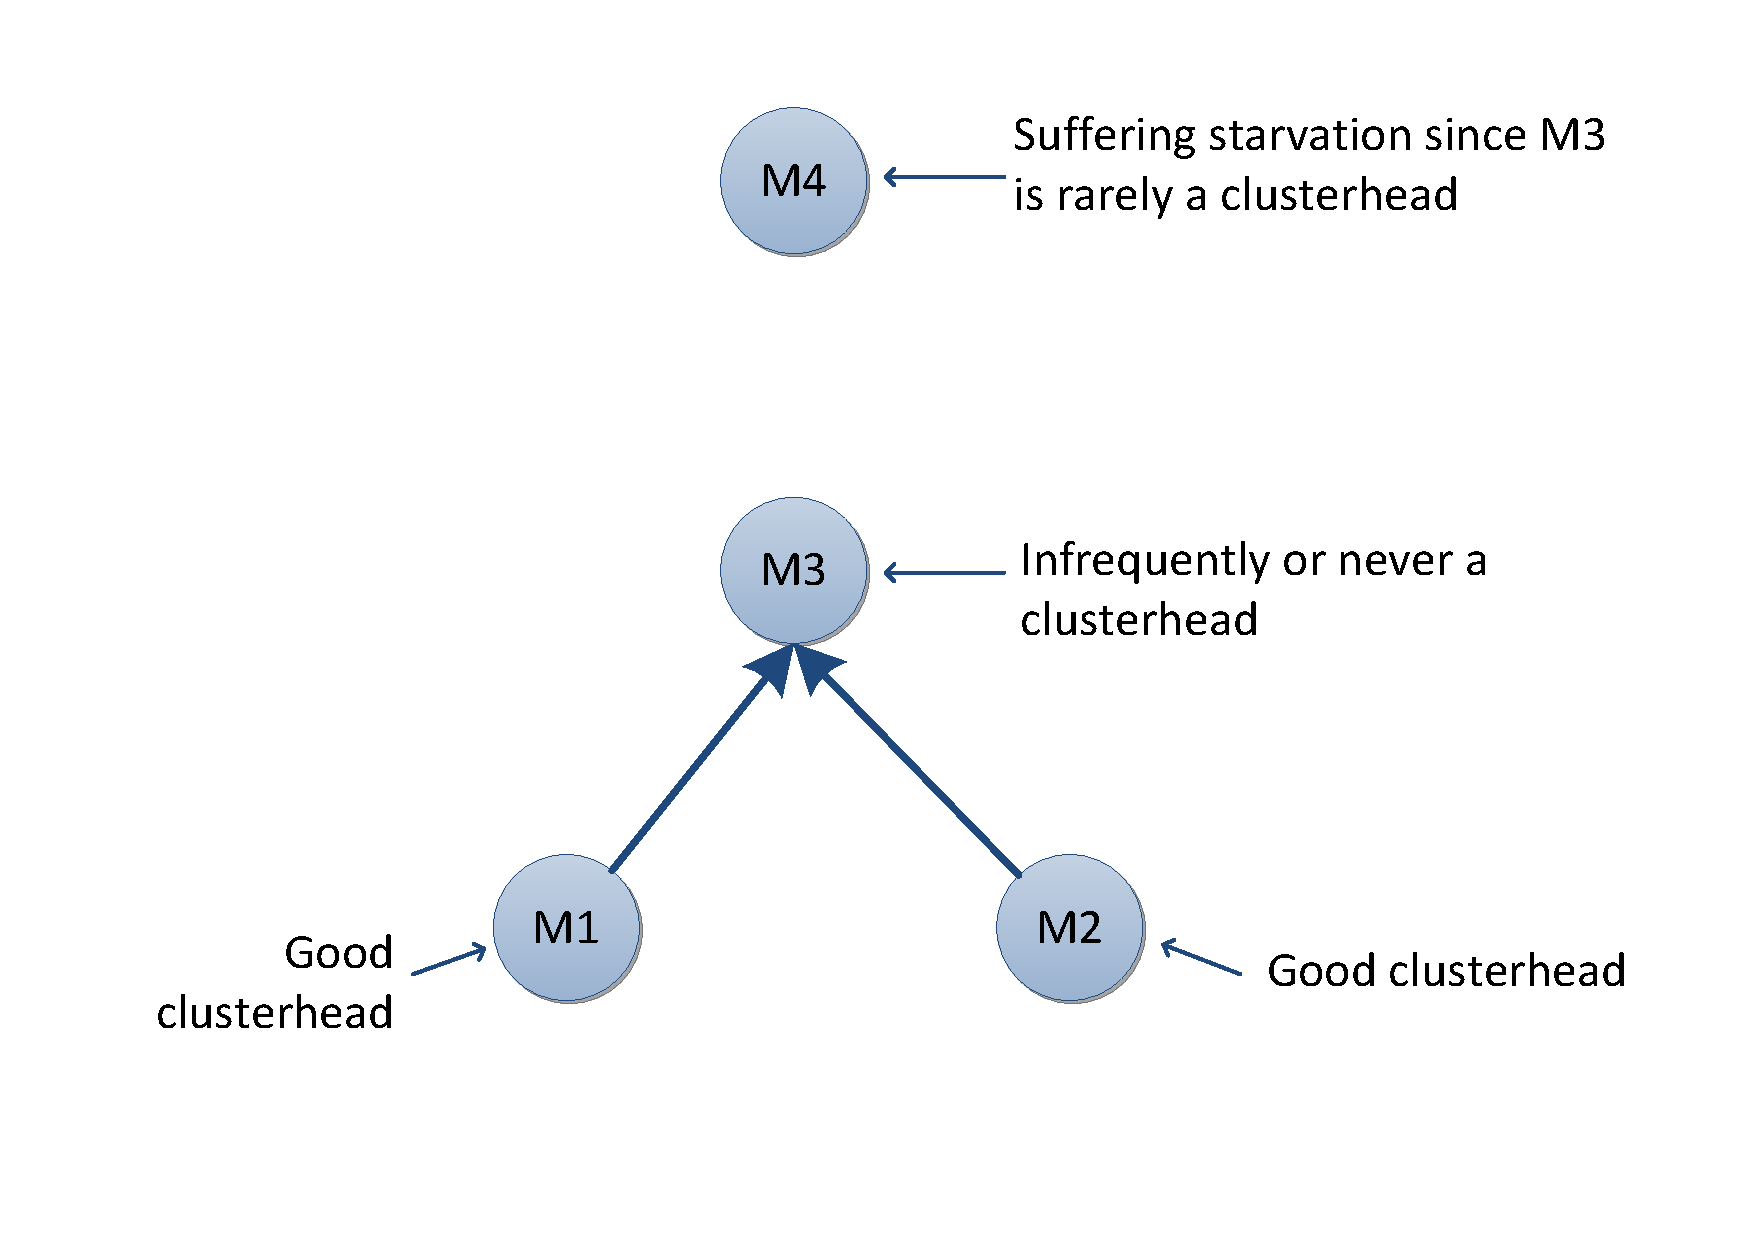
\includegraphics[height=3in]{images/HCCPBlocking/hiddenNode/BetterHiddenNode.pdf}
      	\caption{M3 never becomes a clusterhead since M1 and M2 announce their Clusterhead Candidacy first. Since M3 is never a clusterhead, M4 never has a chance to send its messages through the network.}
      	\label{fig:images_HCCPBlocking_hiddenNode_HiddenNode}
      \end{figure}
     
     
     Conversely, if motes are added to the network after it has run for a while, the HCCP Goodness Delay
     will use much more of the stage time to announce clusterheads, since the new motes will have new batteries and
     empty message queues and therefore have short Goodness Delays, while the old motes will have longer
     Goodness Delays. Due to this, HCCP is very robust to changes after the network has been run for any amount of time.



     
\subsubsection{Suboptimal Clusterheads}
\label{hccp_blocking}

Suboptimal clusterheads are crucial to the success of a network. Starvation can occur in any 
place in the network if a mote is surrounded by other motes that are also poor clusterheads, 
as shown in Figure~\ref{fig:images_HCCPBlocking_hiddenNode_HiddenNode}. Surrounding motes are 
never clusterheads since the surrounding nodes are in radio range of a good clusterhead. The
good clusterhead will advertise itself as a clusterhead, which stops all surrounding motes 
from becoming clusterheads. Since all the surrounding motes are always clustermotes, messages never leave
the mote suffering from starvation. Since this starvation can take place anywhere in the network, it could
be called in-network starvation.

To avoid in-network starvation, all motes should occasionally become clusterheads, even if 
the mote is not well-suited to becoming a clusterhead. Since the mote is not well-suited to being
a clusterhead, this is called becoming a suboptimal clusterhead. Suboptimal clusterheads prevent
in-network starvation by becoming a clusterhead to a mote that is suffering in-network starvation; collecting 
its messages and hopping the messages through the network. 

Due to the timed nature of HCCP elections, suboptimal clusterheads will announce their
candidacy later than good clusterheads. Since the announcement is later, only motes that are suffering
starvation or have no better options (better being defined as a clusterhead that announces earlier or has a lower beacon rank for routing) 
will choose to follow the suboptimal clusterhead. This means that cluster sizes for suboptimal clusterheads should 
be smaller than a normal cluster size. 
If HCCP did not use a timed election, then the cluster for the suboptimal clusterhead's cluster may get too large, sending
too many messages and overrun
the clusterhead's message queue (too many messages received from the cluster), therefore wasting more energy
than needed to 
be a clusterhead.



\subsubsection{Suboptimal First-order Clusterheads}

Since the sink can be considered to be a clusterhead, and is a clusterhead for each round, the motes in radio range of the sink
(called first-order clusterheads)
should be given a different rate of choosing to be a suboptimal clusterhead. A first-order clusterhead is a clusterhead 
that has a beacon rank of 1, that is, is within radio range of the sink.

Since all messages need to be hopped through the motes that are next to the sink, they need to spend more time 
as clusterheads. This is so the first-order clusterheads can receive messages from the rest of the network and 
relay them to the sink.

\subsubsection{Sink Sleep}

Another solution to getting messages to the first-order motes, is to turn
the sink off for a round. Turning the sink off will allow the first-order
motes to become clusterheads. Allowing the first-order motes to be clusterheads
will allow the messages from the network to flow into the first-order motes. Once the 
messages have flowed into the first-order motes, the messages can easily be hopped to the sink.



\subsection{Roundtable Discussion Functions}

As networks were simulated, it was obvious that beacon routing is not efficient at 
sharing the beacon with nodes at the edges of the network. This is due to the fact
that the beacon is shared once per round by the clusterhead. In an optimal case, if
motes have range 100 arbitrary distance units (where range is defined as a radius), a
mote 300 units away would require 3 rounds at minimum to receive a beacon. This
is illustrated in Figure~\ref{fig:images_moteRange_rangeBeacon}
The latency is due to the hopping nature of wireless sensor networks. 
As a beacon is sent out, only the first nodes in range receive a beacon. After that,
the beacon must be sent out from those nodes, and so on. 

\begin{figure}[htbp]
	\centering
		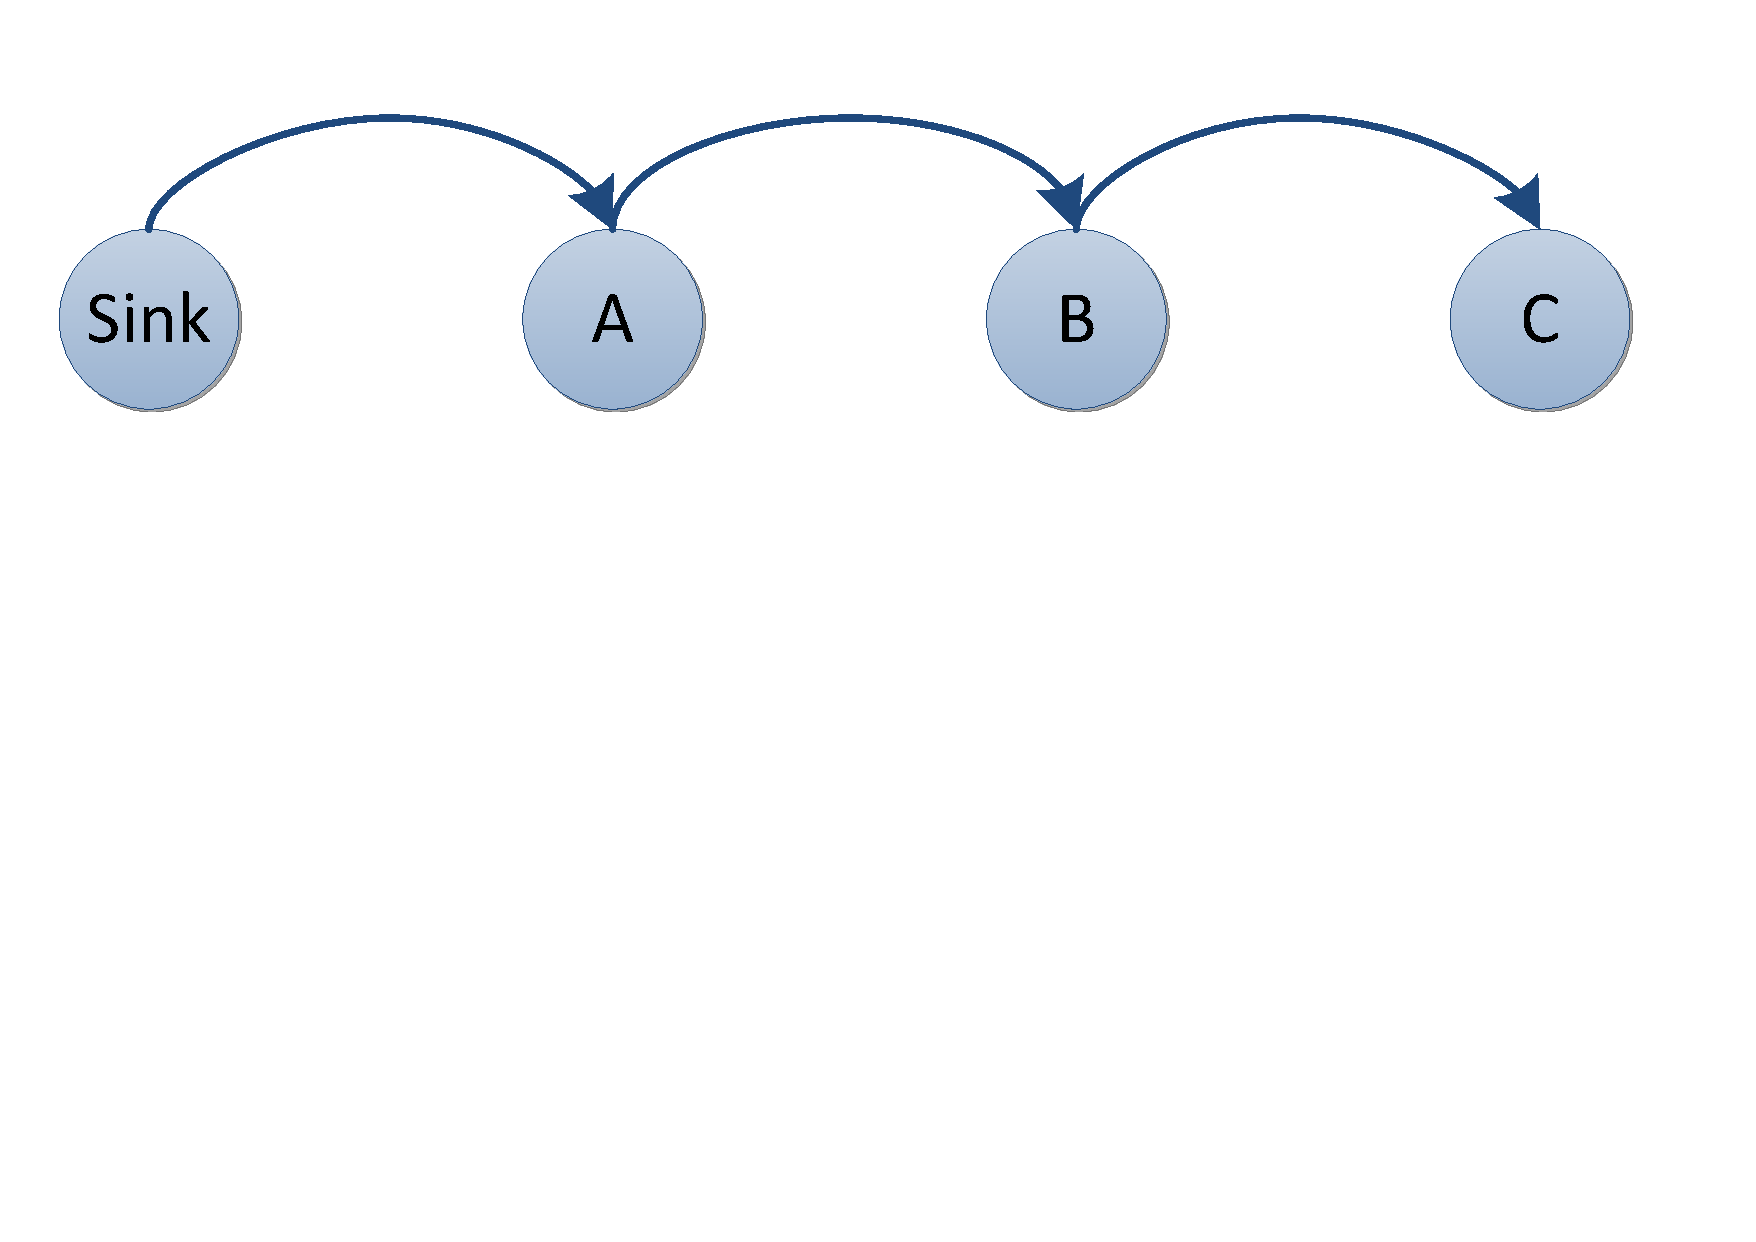
\includegraphics[height=0.6in]{images/moteRange/BetterRangeBeacon.pdf}
	\caption{A mote range 300 away would take at best 3 rounds to receive a beacon given a range of 100.}
	\label{fig:images_moteRange_rangeBeacon}
\end{figure}

To reduce this latency, HCCP uses the Roundtable Discussion to disseminate this important information.
The roundtable time can be used by motes to query for beacons, share beacons and for clusterheads to 
opt out of the clusterhead role. 

A solution to  beacon routing is to flood the network with routing information at every roundtable.
The problem with this would be the number of collisions it would create.  For instance, in a dense network,
if every node were to broadcast its beacon after receiving an update to its beacon, nearly all messages would turn
to gibberish. To prevent this, a balance of density to number of nodes beaconing must be found, or sufficient time 
must be given to the motes for each to beacon without having excessive collisions, making all collided messages overhead.


There are benefits and drawbacks to either method of sharing routing information. Sharing the beacon you received immediately
will cause collisions, but using CSMA can mitigate many of these problems.
Checking to see if the line is clear, doing a CSMA backoff if the line is busy is a simple and effective (though time consuming) way of 
dealing with most of the collisions. Collisions will still  occur, but the worst case is that some motes
might have a beacon rank that is too high.
The mote in the center does not receive a beacon from the closer motes, since the two messages collided.
Two cases can occur from here, either the center mote receives a beacon from a mote further away
from the sink, or re-requests a beacon from the surrounding motes and receives the proper rank.

Overall, the Roundtable Discussion can be a simple exchange of CSMA messages, or can
be made to do specialized tasks as needed by the network. The simulations and testbed
deployments will share routing information using simple CSMA messages.


\subsubsection{Options for Tuning the Roundtable Discussion}
\label{implementationTuning}
The Roundtable Discussion time is very expensive on the network, as all the motes
are on during this time. If a long time is chosen for the Roundtable Discussion, the 
network life will be negatively effected. If a long-lived network is desired, then 
the Roundtable Discussion should be left out all together, as long-lived networks 
are purpose built for lifespan and do not need the energy draw of the Roundtable Discussion.

If no extremely important information needs to be sent during the roundtable time, only a subset of
the motes need to be online to flood the message across the network. This too, will increase the 
lifespan of the network.

\subsection{Clusterhead Choice Timeout}
\begin{figure}[tb]
	\centering
		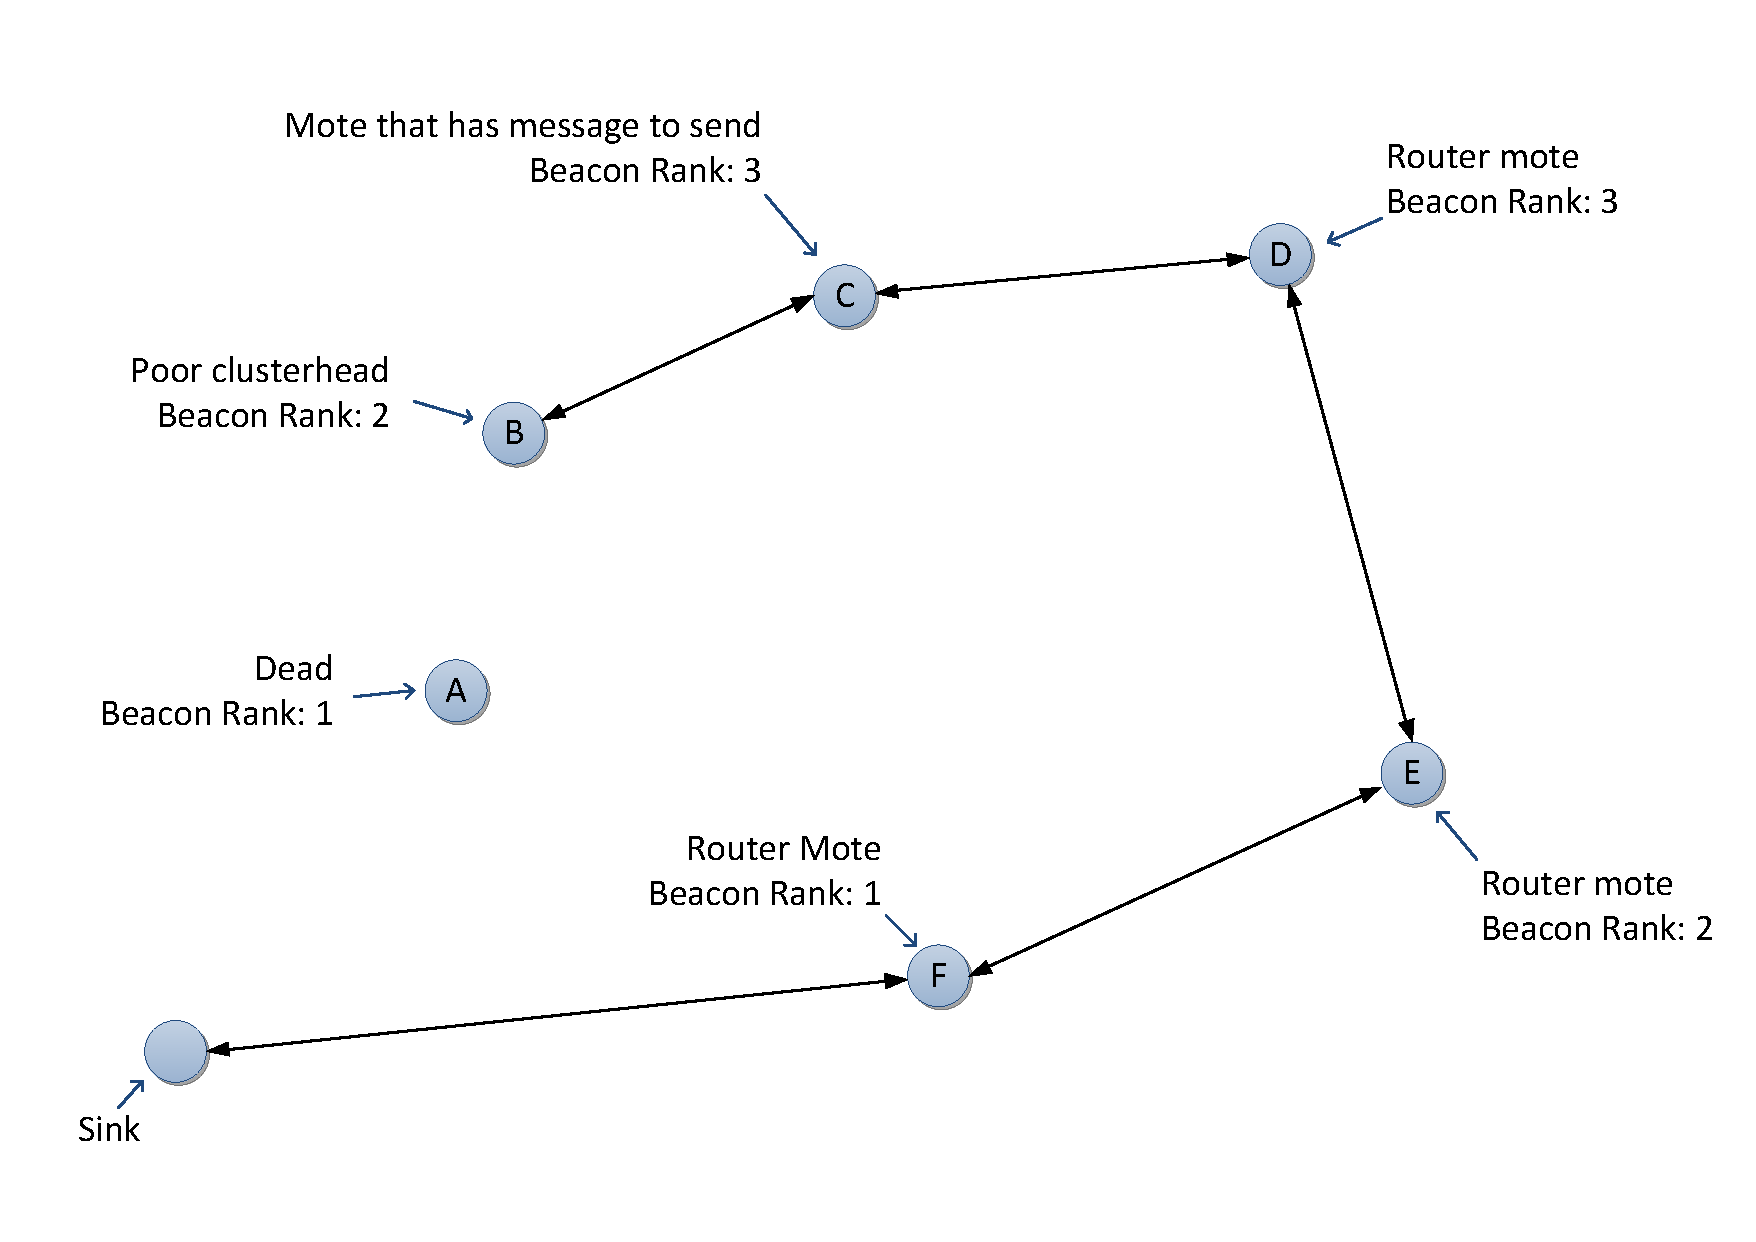
\includegraphics[width=\textwidth]{images/clusterheadChoice/BetterChooseWorseSometimes.pdf}
	\caption{Mote C would should choose mote D as a clusterhead even though mote B is closer to the sink. }
	\label{fig:image_chooseWorse}
\end{figure}



Consider the situation illustrated in Figure~\ref{fig:image_chooseWorse} where a clustermote B has a lower beacon rank than a nearby `very good' clusterhead.
The mote should choose the good clusterhead as its clusterhead over the other potential clusterheads
that may have a better beacon rank, but are significantly poorer clusterheads. 

The question that must be answered is `what is significantly poorer?'. A way to solve this problem is to use
the `Goodness Delay' timing that is already inherent in HCCP. Once a clustermote has heard a clusterhead announcement, there is a
timeout clock that starts. If another clusterhead makes an announcement before the timeout expires, and that new clusterhead 
has a lower (better) beacon rank, the mote should join that new cluster. Once the timeout has expired the quality clusterheads
that are announcing are considered significantly poorer than a known clusterhead. This is due to the `Goodness Delay' that HCCP 
uses to discover heterogeneity in the network. So, despite a mote having a lower beacon, it might not be the best clusterhead, and the 
clusterhead that is good should be used.





\chapter{Experimental Setup and Results}
\label{ch:expresults}


Simulations and a testbed deployment were created to show the benefits of using HCCP over LEACH
and were used to compare the two protocols. 
To compare the performance of HCCP and LEACH, simulations were created for both of them using custom
simulation software. The simulation software is freely available on Github at (\url{http://github.com/robguderian/hccp}).
The simulation provides a high-level view of a WSN, focusing on  
how the network can function together and give insight into the network, allowing 
many different factors to be logged that would otherwise be impossible to track.

For the testbed deployment, both HCCP and LEACH code were created for four 
different types of WSN motes that have the ability to communicate with 
each other. A small deployment was then run to help show that 
the simulations are accurate and that HCCP can work
in a real-world environment.


\section{Simulation of HCCP and LEACH}
\label{ch:sim}


A custom simulator was developed to simulate the running of HCCP. Other network simulation suites
are available, such as OmNet++~\cite{omnet} with its related suites such as Castalia~\cite{castalia}  are
widely used, and provide tools for analysis. These tools were tested, and were deemed unfit for the 
desired simulation setups. Tracking the number of messages sent, from where, route taken and 
number of times a given message has been received at the sink are possible, but difficult to collect.
OmNet++ messages can only be in one mote's message queue at a time since it can only have one `owner'.
Since a message can only have one owner, it is very difficult to track how many times a given 
message has been received at the sink. Also, the MAC layer protocol is not simple to change while
running a simulation. LEACH uses both CSMA and TDMA MAC protocols, so to properly simulate LEACH either 
switching the MAC protocol must occur, or the finer details of the protocols must be abstracted and be viewed simply as access to a radio. 


WSN code can be written 
in such a way that the physical layer can be largely ignored. 
The physical layer controls the  radio, modulating the 
frequency to communicate with surrounding motes. This includes
what frequency or protocol (such as 802.15.4 or ANT radios) the motes use.
The simulator abstracts the physical layer, as it is not the focus of the
simulation or research. 
It is assumed that the radios work, have a given range and draw 
power when on.

When building the simulator, the problem of simulating a WSN was viewed as 
a queuing theory problem more than a networking problem. In doing this, many of 
the network problems are abstracted away, such as radio channels or how collisions can be 
recovered from. HCCP currently only uses one radio channel, so only one channel was
created. Messages that have collided are assumed lost, and unrecoverable.

With these assumptions and abstractions, a simple to understand simulation could be made 
to collect important statistics about the inner workings of the network.



\subsubsection{Simulator Capabilities}
The custom simulator is able to create networks of any size with a two dimensional rectangular space in which
to place the motes. Attention was given to the use of random number generators and 
randomly created events. Random seeds are kept, and random events can happen at the 
same times in networks that are being compared. 

Each mote is given its own random number generator with its own seed to generate random events. 
Separate random number generators are used to draw random numbers for all tasks, ensuring
the simulated motes generate the same random numbers for both the LEACH and HCCP simulations.

The package used to generate random numbers, and to maintain the event queue was SSJ~\cite{SSJ}. 
SSJ is a well-respected Java simulation package. The pseudorandom number generator and the
event queue were built for simulating queuing theory events, and therefore were easily applied to simulating
events in wireless sensor networks.

SSJ provides excellent facilities for collecting statistics on the motes. SSJ can collect continuous 
data, such as calculating what percentage of the time a given mote was on or off; or, collect discrete
events, such as number of messages received, sent and lost.


\subsubsection{Design of Motes in the Simulation}

The custom simulator simulates motes that are an abstraction of motes in real life.
Motes have been abstracted to have the following features:
\begin{enumerate}
	\item \textbf{A battery}: The battery drains faster when the mote is on, and slowly when the mote is sleeping. 
	Motes can draw more power if they are power intensive motes, or less power if they are power efficient motes.
	The batteries can start with more or less energy, which simulates having a larger or smaller battery. Since batteries in
	reality do not always have the same amount of battery power, the 
	simulator applies jitter to the amount of power given to the motes. This amount is configurable, and generally
	assumed to be quite small.
	\item \textbf{A message queue}: The queues contain messages created by this mote, and messages that have hopped into this mote. The 
	queue has finite space. If the queue is full, the message that should be added to the queue is lost.
	\item \textbf{Sensor readings}: Sensor readings happen at a specified frequency. Sensor readings get turned into 
	messages which are added to the message queue. If the message queue is full, the message with the reading is 
	lost.
	\item \textbf{A simple MAC layer}: The MAC layer is designed to be simple and abstract. CSMA uses backoffs of the
	channel is currently being used. CSMA waits a random amount of time before attempting to send the message again. 
	Each mote needs its own random number generator to generate a random backoff time.
	\item \textbf{A radio}: All devices have radios that have a given range. If a neighbouring mote is within range of 
	a device, the two motes can communicate. All radio links are assumed to be one-way links, as some radios
	could have more transmission power than other radios. The units of the range are arbitrary distance units, 
	and could be interpreted as centimetres, metres or even miles.
	\item \textbf{A position}: Motes are given a position on the two dimensional plane. Any mote can be set to 
	be mobile in the network, and can move at any time. This movement will change which surrounding 
	motes the moving mote can communicate with.
\end{enumerate}
This is consistent with the high-level description Akyildiz et al.~\cite{wsnSurvey} gave
to describe a mote, and with Figure~\ref{fig:images_intro_mote}.

Motes can be of various different types: basestations, routing nodes, or sensor nodes. Basestations
are the sinks, once a message is received at the basestation it is marked as completed.  Routing nodes
are motes that have no sensors, and are therefore ideal  for routing messages. Sensor nodes are
motes that make sensor readings, and the sensor readings are turned into messages. The type
of sensors and number of sensors have been abstracted away. Basestations are assumed to have wall power, sensor and routing 
nodes are generally assumed to have battery power, but the simulator has the capabilities of giving them wall power.

Heterogeneity is given to the motes by initializing the motes with different properties, such as:
\begin{itemize} 
	\item more or less battery power 
	\item more or less power drawn when on or off 
	\item more or less available space for a message queue
	\item longer or shorter radio transmission range
	\item the ability to move or not and how fast the movement is
	\item frequency of sensing and creating messages
\end{itemize}

The number of sensors or type of sensors can be abstracted to being a frequency of sensing events. If a mote has many sensors, 
it can be abstracted to have more sensing events. A routing mote is the other extreme, in that a routing mote has 
no sensing events and therefore no frequency of sensing events.

All motes in the custom simulation use common code for the MAC layer, as this is a requirement for heterogeneous WSN. Motes in heterogeneous
WSNs have differing hardware, energy levels and capabilities, but share a common mode of communication.

\paragraph{Motes in the Simulations}

A set of motes were reused for consistency across all the simulations. This provides 
standardization of the motes across the simulations while providing heterogeneity across
the simulations. The power draw of all the motes were kept the same across all the types of motes
for all simulations. The motes varied in queue size and battery size.

\begin{itemize}
    \item \textbf{Router} - A special type of mote that does not have any sensors. It is given a large queue and a large battery making it ideal for routing messages.
    \item \textbf{Normal} - An average mote. Most of the motes in the network are set to this kind of mote. It has an average battery, and an average queue.
    \item \textbf{Expensive} - The expensive mote simulates a mote that has expensive sensors that are power hungry devices. This mote has a larger message queue than the normal mote, but a smaller battery.
    \item \textbf{Very Expensive} - The very expensive mote simulates a mote that has more power hungry sensors than the Expensive mote,  a smaller battery, and a smaller message queue.
    \item \textbf{Super Expensive} - The Super Expensive mote simulates a mote that has the most expensive sensors that put a very large load on the battery. It therefore has the smallest battery, and the smallest message queue.
\end{itemize}

\subsection{Modifications to LEACH for Simulation}
LEACH does not specify which routing algorithms should be used when using LEACH.
For comparison reasons, two routing algorithms were used in creating LEACH: beacon routing 
and 
preset routing, where every node knows its beacon rank from the beginning of the simulation.

In the beacon routing implementation, the mote published its beacon rank when it announced 
it was a clusterhead, during the clusterhead announcement phase. This is not very efficient, but is
a realistic way
of disseminating the routing information to the network.

Since HCCP has facilities to efficiently disseminate routing information, a preset routing simulation was created. The
preset routing simulation sets each of the motes appropriate beacon rank before the simulation starts. This permits the network to work
as if the network has been alive for long enough that the routing information has been disseminated thoughout the network.


\subsection{Modifications to HCCP for Simulation}
HCCP has facilities for routing, but does not specify which routing algorithm should be used. 
Because a routing algorithm is needed for the network to work once it is deployed, the simulation has 
been implemented with beacon routing with HCCP, as HCCP will then be evenly comparable to LEACH. 
The beacon information is disseminated during the roundtable
discussion, as prescribed by HCCP.

Since LEACH has been provided preset routing, the HCCP simulation has also been 
given preset routing, so it can be fairly compared to LEACH. Simulations with
the preset routing tables were done, as were simulations without preset routing tables 
to show the differences in data dissemination between the networks.

% NOTE TO SELF: fake routing is pre-filling the routing tables - CALL IT preset routing



\subsection{Observations and Results}


The worst-case baseline runtime for a mote in the simulation setup is 40,776s (the mote is always on), and the best-case runtime is
256,200s (the mote is only on during the mandatory times). Clearly the best-case is impossible to reach, as all motes would be sleeping 
for the entire cluster runtime (TDMA schedule runtime), never sending any data messages. 
Since the motes are asleep for the entire cluster runtime,  it will also will
never send hop messages, which means the mote will never have its messages reach the sink and is therefore useless. If 
a mote is always a clusterhead, it will be on for the entire simulation making the worst-case runtime a possibility in 
the simulation. Duty-cycling ensures that a mote will never only run as a clusterhead.
% onDraw					1.5
% update 		60
%  500 * 400 
%  81 * 600 avg battery = 427
%  427/1.5
% 427*0.1
% 5 / 5.55
%= 0.9009009009009
%0.55 / 5.55
%= 0.0990990990991
%17080 * 0.9009009009009 + 256200 * 0.0990990990991
%= 40776.5765765768
%
% 
% 



All permutations of the possible Goodness Delay factor configurations were run to provide insight to which 
HCCP parameters that build the Goodness Delay  (described in section~\ref{subsec:goodnessDelay}). 
The permutations were run as the following: 100\% Battery power; 99\% Battery power, 1\% Message queue; 99\% Battery power,
1\% Random; and so on.
Each parameter contributes a percentage of the time that the mote waits before it 
announces its Clusterhead Candidacy or Clusterhead Announcement. Since there are 5 factors,
each are considered separately. The LEACH-style clusterhead percentage is controlled separately from the 
5 HCCP factors and are also viewed separately. Motes will elect to be a Clusterhead Candidate using the same
equation as LEACH uses for electing clusterheads.

The $x$-axis of the following graphs show the percentage that the listed HCCP factor contributes to the
Goodness Delay. The remainder of the Goodness Delay is a permutation of the remaining HCCP factors. For instance:
if the contribution to the Goodness Delay of Battery Power is 50\%, the other 50\% will be made of up all the 
possible permutations of Random, Duty Cycle, Message Queue and Sensor Mission. 
The charts all have the same $x$ and $y$ axis to make comparisons clearer. 


\begin{figure}[htb]
	\centering
		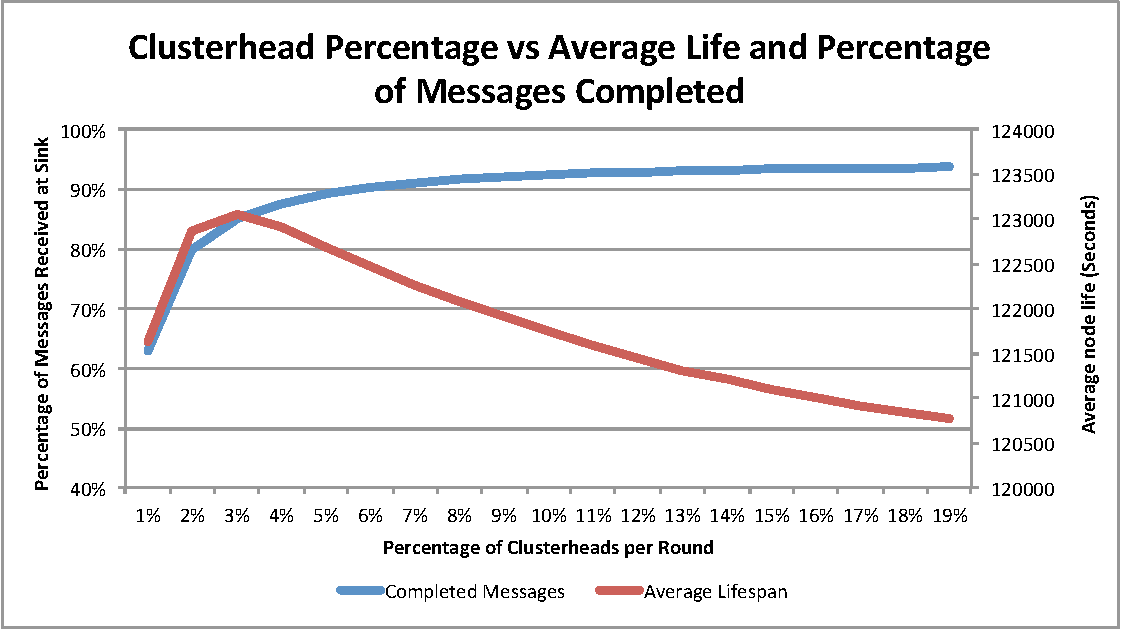
\includegraphics[width=6in]{images/simulation/goodness/clusterhead.pdf}
	\caption{Visualization showing the relationship between Percentage of Clusterheads per round and simulation results.}
	\label{fig:images_simulation_goodness_clusterhead}
\end{figure}


HCCP, much like LEACH, can be set up to vary the percentage of clusterheads per round in the network.
Since motes that are clusterheads use more power per round than motes that are not clusterheads, choosing
a higher percentage of clusterheads per round causes the network to have a shorter lifespan. This effect can 
be seen in Figure~\ref{fig:images_simulation_goodness_clusterhead}, as the percentage of clusterheads increases the 
lifespan of individual motes drops. There is a peak at 3\% clusterheads for average lifespan since motes that choose clusters
turn off for the remainder of the HCCP phase. These small energy savings add up to make the average lifespan of the network 
longer. Heinzelman et al.\cite{leach} also saw the same phenomenon happen while testing LEACH, finding that the motes
dissipate the least energy in their test case at about 5\% clusterheads per round. Since HCCP uses many of
the design elements of LEACH it is not surprising that the two have similar optimal percentages of clusterheads
per round. 

The message throughput increases with the percentage of motes that are clusterheads each round. This makes sense,
as the non-clusterhead motes would have a good selection of clusterheads to choose from, and could choose a
clusterhead that is nearby to decrease the chances of a message collision. However, as the percentage of clusterheads
increases, the lifespan of the network decreases. This causes a tradeoff for a network administrator to choose from, 
as some networks might require longer lifespans, while other networks may value message throughput.

\subsubsection{Effect of Goodness Delay on HCCP}

\begin{figure}[htbp]
    \centering
        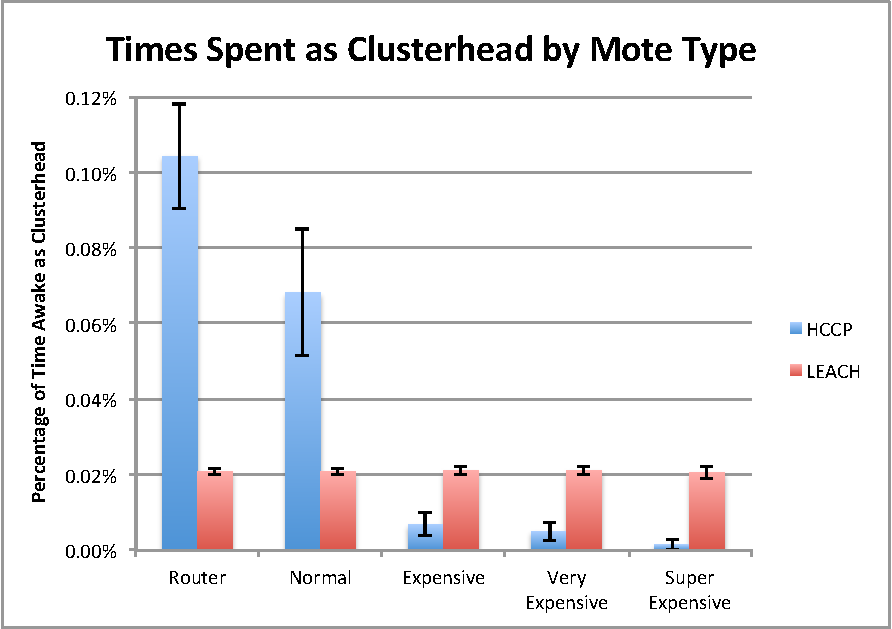
\includegraphics[height=3in]{images/clusterheadChoice/SensorMissionCHTime.pdf}
        % from charts/sensorSmall/nodedata.xlsx
    \caption{The Goodness Delay focuses the clusterhead task on motes that are suited for the task.}
    \label{fig:images_clusterheadChoice_SensorMissionCHTime}
\end{figure}

The Goodness Delay in HCCP is intended to make motes that are well-suited for the task
clusterheads more often. Figure~\ref{fig:images_clusterheadChoice_SensorMissionCHTime} shows
that the Goodness Delay is effective in doing this. As the motes get more expensive, hypothetically
with more power-hungry sensors, the mote gets chosen to be a clusterhead less frequently. This means that 
the mote will draw less power, since it is not being a clusterhead as frequently. 

Note that in Figure~\ref{fig:images_clusterheadChoice_SensorMissionCHTime} the percentages are quite low, as
the the Y axis is the percentage of time  the mote was a clusterhead over the entire
time it was alive, which includes long sleep periods between cycles of the protocol.



\subsection{Discovering how Heterogeneous Factors Effect the Network}
Simulations were run with all the possible permutations of
the factors available in the simulation. The results show which heterogeneous
factors are valuable for improving the WSN. The factors that could be used in 
clusterhead elections in HCCP are: residual battery power, 
available message queue size, sensor mission, when the last time this node was a 
clusterhead was, and a random variable. Breaking the problem down to the separate factors, 
the value of the factors can be compared.


All the permutations of the HCCP factors for Goodness Delay were run on the same network
with the same random seeds. This set up the network with the same starting and running parameters so
that events would happen at the same times in the various networks, allowing the networks 
be comparable 
with the given parameters.

\subsubsection{Effect of Available Queue Size on HCCP Goodness Delay}


Focusing on available queue size for a method of describing how good a mote would do as a clusterhead
is an obvious choice, as clusterheads will be collecting messages from the surrounding motes and need the 
ability to store all the messages. If the message queue is full on a mote, it could not store the new incoming messages, therefore
losing all incoming messages. If incoming messages are lost it not only is negative to the network in terms of information loss,
 but also wastes the energy of the poorly chosen clusterhead and all the motes that register with that cluster.

 \begin{figure}[bthp]
 	\centering
 		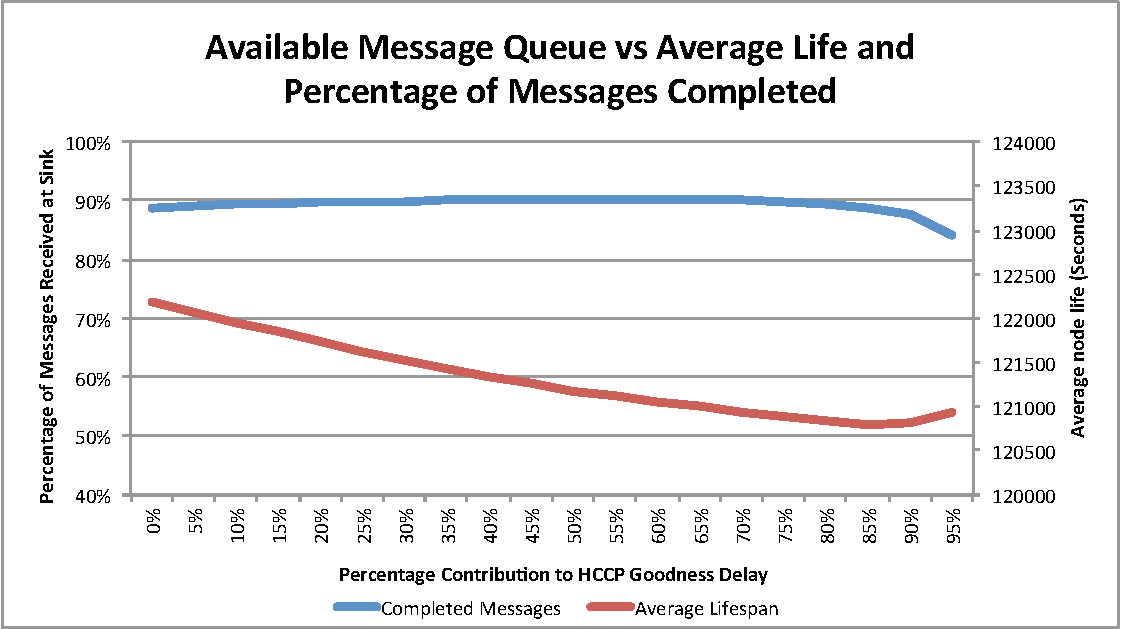
\includegraphics[width=0.9\textwidth]{images/simulation/goodness/AvailableQ3.pdf}
 	\caption{The relationship between HCCP Goodness Delay using Available Queue size and simulation results.}
 	\label{fig:images_simulation_goodness_AvailableQ}
 \end{figure}


The effects of focusing on Message Queue size can be seen in Figure~\ref{fig:images_simulation_goodness_AvailableQ}. 
As the focus on message queue increases, the average lifespan of the network drops. This is not surprising as the focus
on battery power and duty-cycling reduces, making the network solely focus on choosing clusterheads that have
large available message queue size regardless of available power. Because of this, Message Queue size is likely a good 
secondary factor that would control less of the Goodness Delay, balancing a factor such as Battery Power.

% charts/10-1000freqtest
\begin{figure}[htbp]
    \centering
        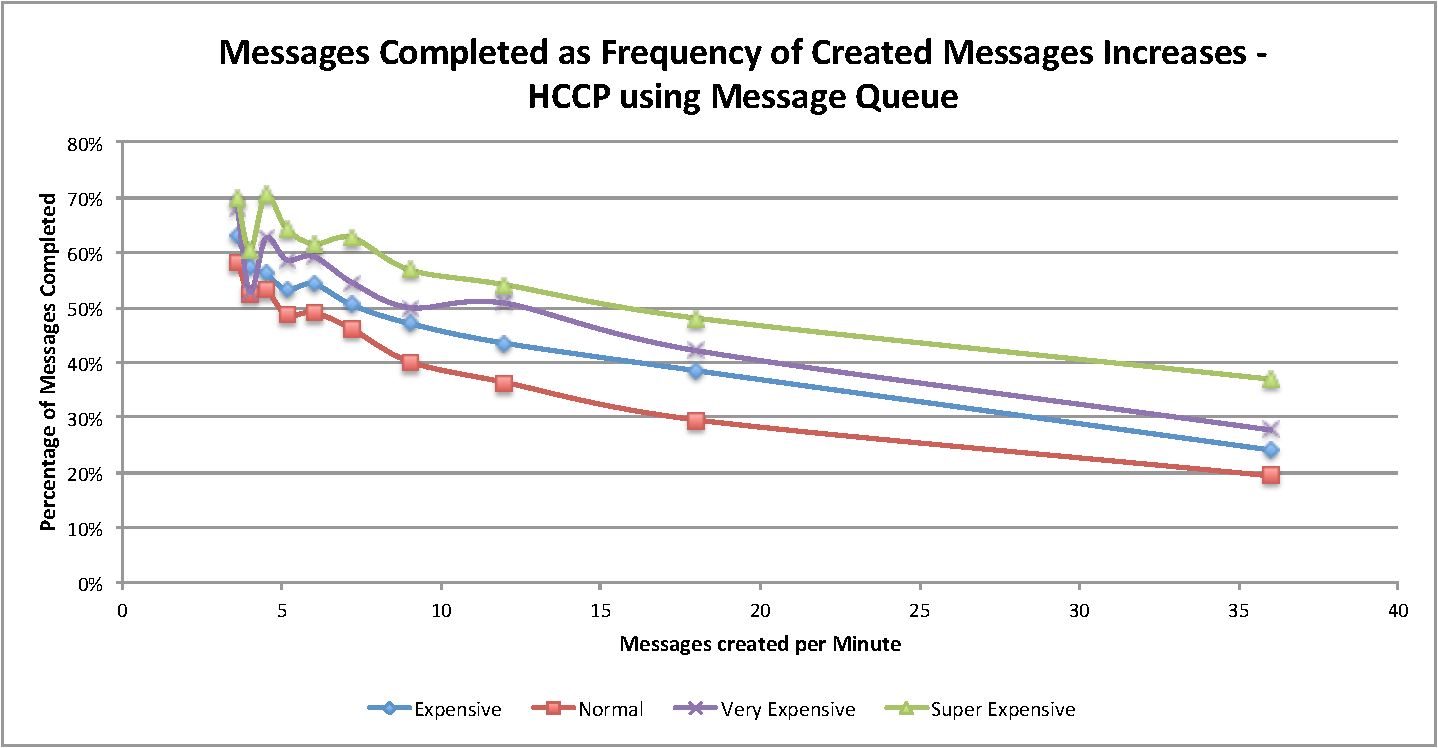
\includegraphics[height=3in]{images/messageFrequency/HCCP.pdf}
    \caption{HCCP handles being overloaded with messages well, as motes with larger available message queues will opt to be clusterheads.}
    \label{fig:images_messageFrequency_HCCP}
\end{figure}

\begin{figure}[htbp]
    \centering
        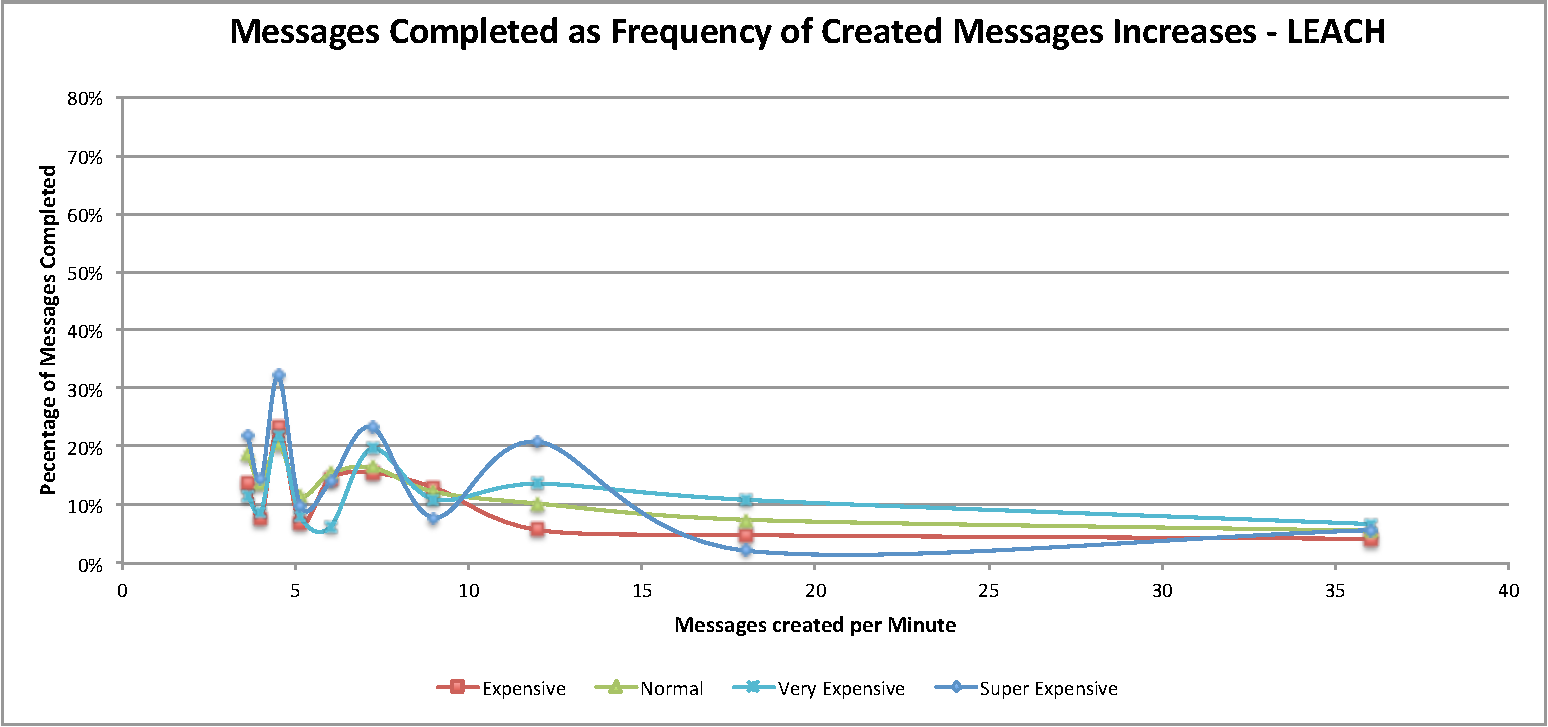
\includegraphics[height=3in]{images/messageFrequency/LEACH.pdf}
    \caption{LEACH does not handle being overloaded, as it does not consider message queue size when electing clusterheads. Note the $y$ axis is the same as Figure~\ref{fig:images_messageFrequency_HCCP}.}
    \label{fig:images_messageFrequency_LEACH}
\end{figure}

As the network gets busier, the chances of any mote having a full message queue is greater. When message queues
start filling up, the importance of focusing on message queue size as a HCCP Goodness Delay factor increases. 
Because HCCP can focus on which motes can be effective clusterheads, better clusterheads will be elected.
The results of this can be seen in Figures~\ref{fig:images_messageFrequency_HCCP} and~\ref{fig:images_messageFrequency_LEACH}, which 
have the same $x$ and $y$ axes to show the difference between the two results.
HCCP can handle a network that is overloaded with messages quite well, because motes with more
available space to hold incoming messages from the clustermotes will be more likely to be clusterheads.

The standard deviation of the simulation is approximately $\pm$20\% for both HCCP and LEACH for each
frequency level. This shows that HCCP focusing on Message Queue has a significant gain over LEACH
in terms of message throughput for Super Expensive motes even at the most overloaded network run. It is 
also interesting to note that the signal-to-noise ratio for LEACH is approximately 100\%, even 
at the least overloaded simulation run.


\begin{figure}[htbp]
    \centering
        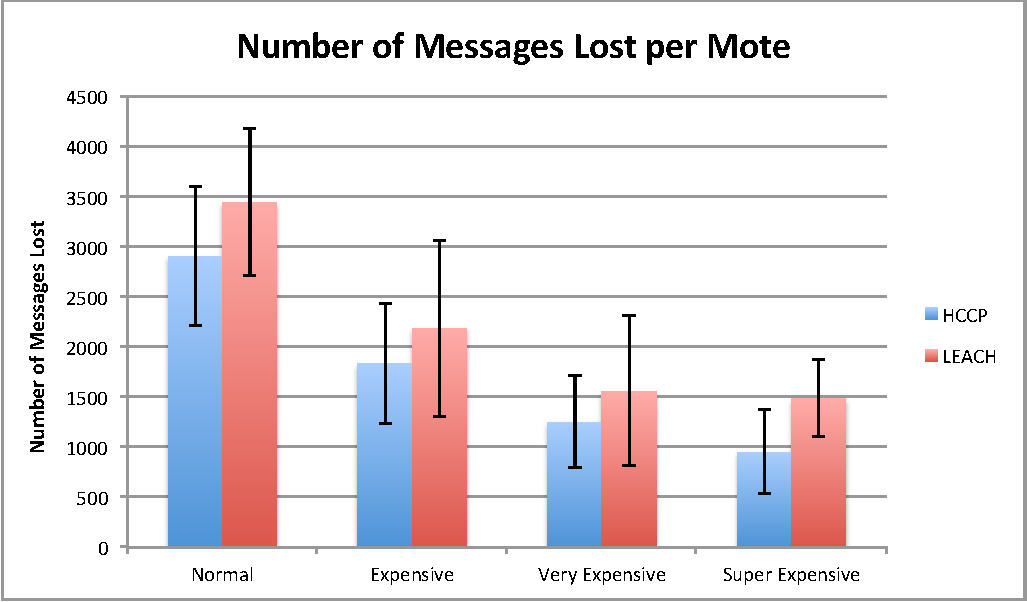
\includegraphics[height=3in]{images/messageFrequency/MessagesLost.pdf}
    \caption{HCCP loses fewer messages due to full message queues than LEACH.}
    \label{fig:images_messageFrequency_MessagesLost}
\end{figure}

HCCP focusing on Message Queue will have the effect that fewer messages 
will be lost due to having no available space in the message queue.
Fewer messages will be lost as motes that have more available message queue space will opt
to be clusterheads, which will then free up space in the surrounding motes to use.
Figure~\ref{fig:images_messageFrequency_MessagesLost} shows that HCCP does 
have fewer lost messages, significantly more for Super Expensive motes. 
This shows that HCCP has gains over LEACH in how many messages are lost due to 
full message queues.

\subsubsection{Effect of Available Battery Power on HCCP Goodness Delay}


Choosing motes with more available battery power creates network with long average lifespans, as seen in 
Figure~\ref{fig:images_simulation_goodness_Battery2}. Comparing Figure~\ref{fig:images_simulation_goodness_Battery2} to 
Figures~\ref{fig:images_simulation_goodness_clusterhead} \ref{fig:images_simulation_goodness_AvailableQ} \ref{fig:images_simulation_goodness_Duty}
and \ref{fig:images_simulation_goodness_Random} it is clear that focusing the HCCP Goodness Delay on available battery 
power is second only to Sensor Mission without the drawback of having to know any information about the
network before deployment. 

\begin{figure}[htbp]
	\centering
		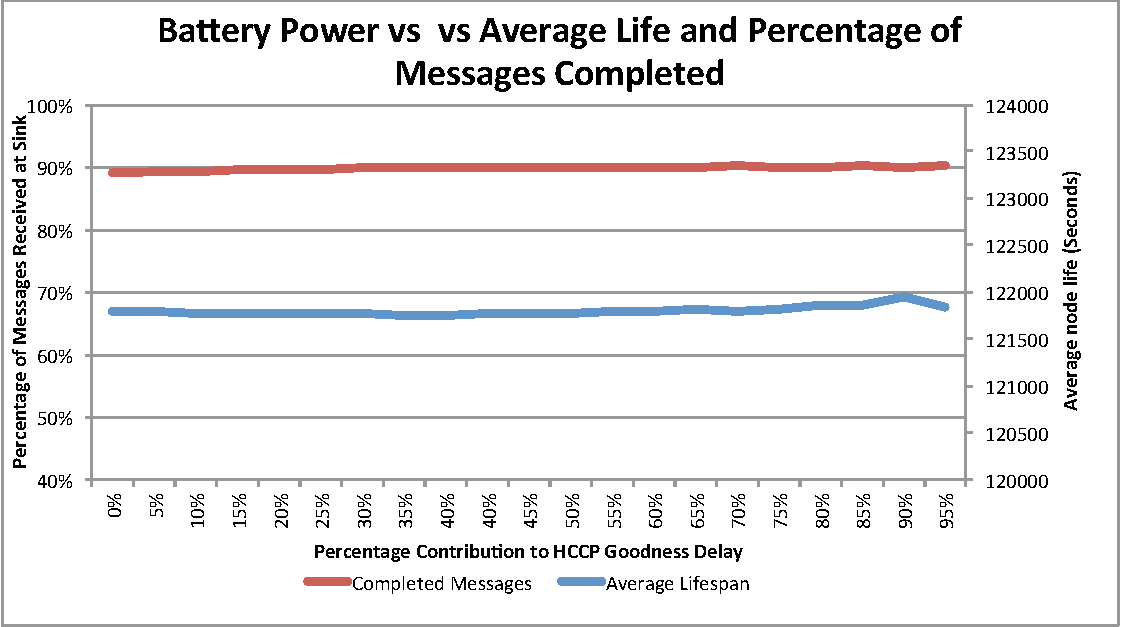
\includegraphics[width=0.9\textwidth]{images/simulation/goodness/Battery4.pdf}
	\caption{The relationship between HCCP Goodness Delay using Available Battery Power size and simulation results.}
	\label{fig:images_simulation_goodness_Battery2}
\end{figure}


An interesting result of focusing on Battery Power is that fewer messages are lost
due to motes dying. This makes sense, since as the battery in the mote nears depletion, 
the mote will not elect to be a clusterhead. Because the mote is not a clusterhead, the 
mote is not accepting messages from surrounding motes, rather it is getting rid of 
all the messages in its message queue. Then, once the mote finally dies, its 
message queue will be as empty as possible and minimal messages are lost.  

This
effect can be see in in Figure~\ref{fig:images_simulation_BatteryVsLeach_Death}.
The election protocol in LEACH is naive, electing clusterheads at random, causing
motes that are nearing death to become clusterheads. Notice that there is a 
high variability in how many messages are lost in dying motes in LEACH. 
In fact, the simulation results showed that there were motes that
died with their message queues completely full. HCCP, on the other hand,
has very low variability due to the network avoiding using dying motes as clusterheads.

The end result of using Battery Power as an HCCP factor, is that fewer messages are lost, 
therefore more messages successfully reach the sink. This can be seen in 
Figure~\ref{fig:images_simulation_BatteryVsLeach_Messages}.

\begin{figure}[htbp]
    \centering
        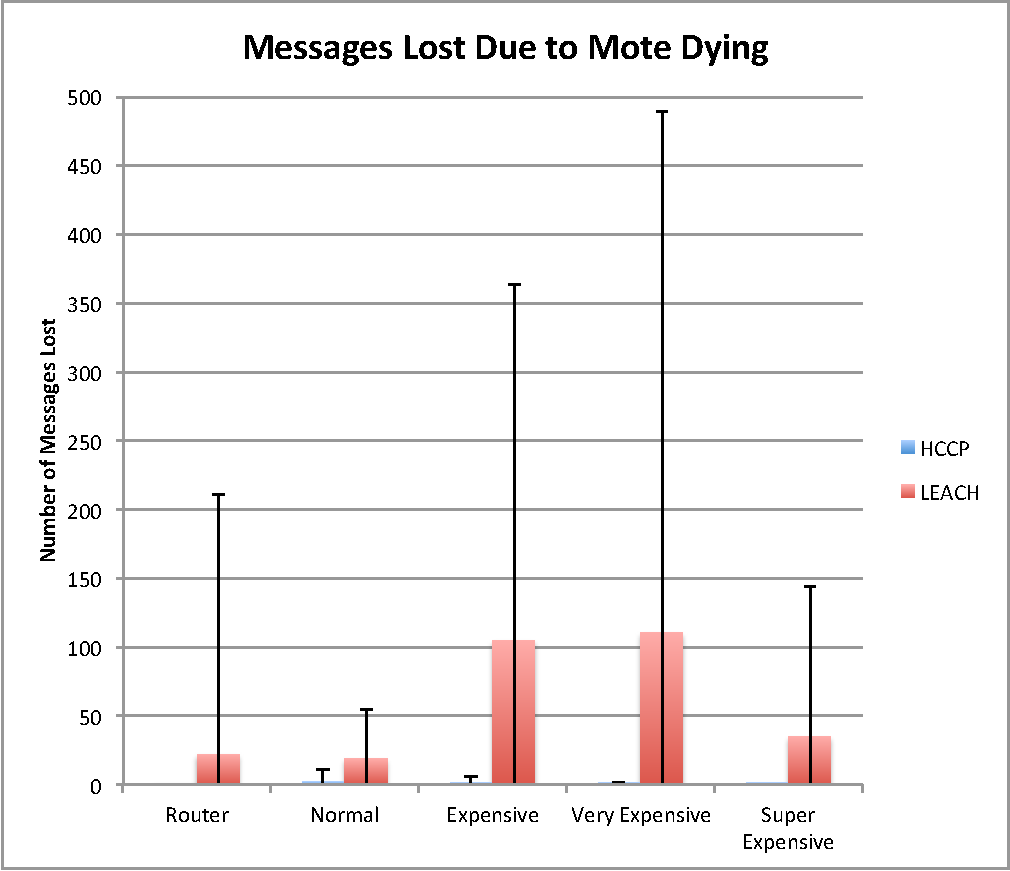
\includegraphics[height=3.75in]{images/simulation/BatteryVsLeach/Death.pdf}
    \caption{HCCP focused on Battery Power loses less messages since dying motes will not elect to be clusterheads.}
    \label{fig:images_simulation_BatteryVsLeach_Death}
\end{figure}

% from /Users/robg/charts/BatteryVsRandom4-noSinkSleep/
\begin{figure}[htbp]
    \centering
        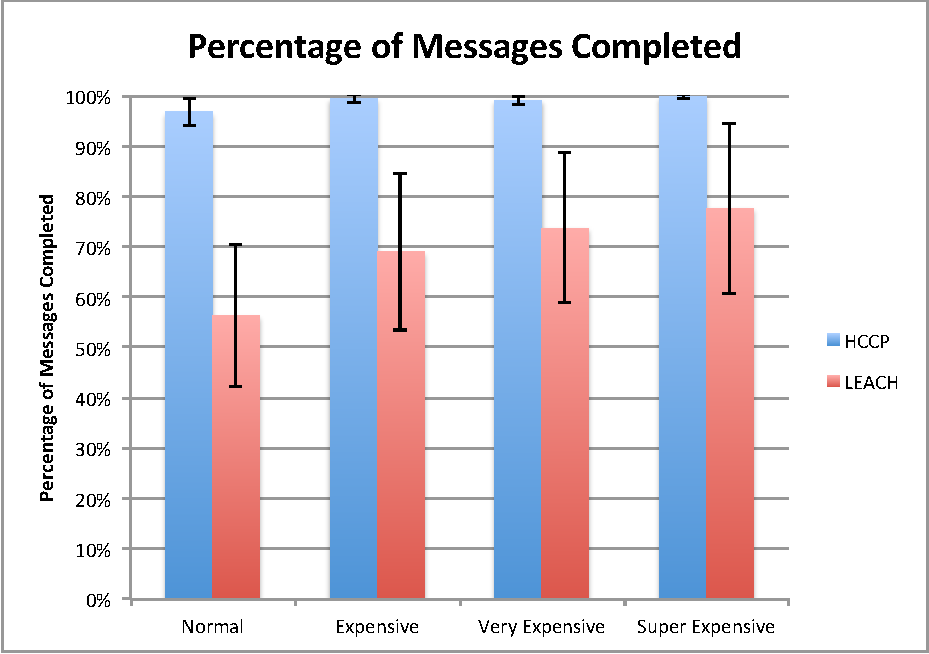
\includegraphics[height=3in]{images/simulation/BatteryVsLeach/Messages.pdf}
    \caption{HCCP focused on Battery Power has better throughput than LEACH since fewer messages are lost in dying motes.}
    \label{fig:images_simulation_BatteryVsLeach_Messages}
\end{figure}



\subsubsection{Effect of Duty Cycling on HCCP Goodness Delay}

\begin{figure}[htbp]
	\centering
		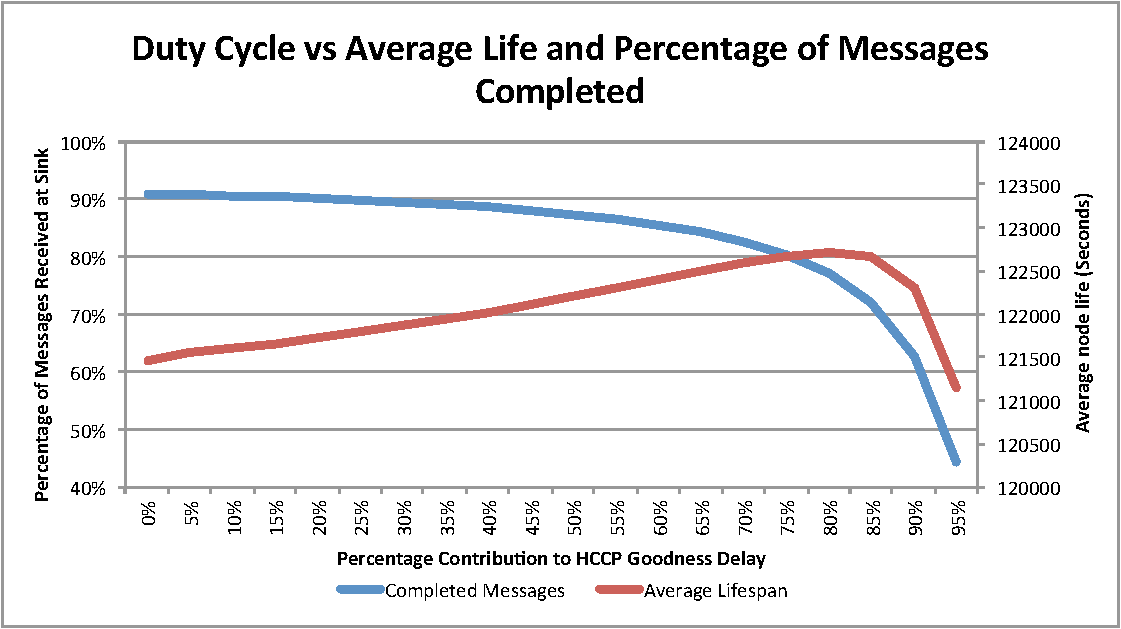
\includegraphics[width=0.9\textwidth]{images/simulation/goodness/Duty2.pdf}
	\caption{Visualization showing the relationship between HCCP Goodness Delay using Duty Cycling and simulation results.}
	\label{fig:images_simulation_goodness_Duty}
\end{figure}

The HCCP Duty Cycle factor causes motes to live longer, but deliver fewer messages. This is the
common WSN throughput versus lifespan tradeoff. As motes focus on duty-cycling, they 
become clusterhead less frequently, which causes message throughput to drop. This 
relationship can be seen in Figure~\ref{fig:images_simulation_goodness_Duty}, as 
the focus on Duty Cycling increases, the message throughput drops while the average mote lifespan 
increases. This trend is followed until 85\% focus on Duty Cycling, at which time the same effect as 
clusterhead percentage in LEACH occurs, too few motes are announcing themselves as clusterheads, causing 
the rest of the motes to be powered up longer waiting for clusterhead candidacy and clusterhead announcement messages.
Since these motes are on longer waiting for announcement messages, the lifespan drops. Though there are obvious 
gains for life span to focusing on Duty Cycling, Duty Cycling is a better secondary HCCP Goodness factor with a 
minority of the control of the Goodness Delay time.

The problem with Duty Cycle as the main HCCP Goodness factor is that it is not 
providing enough value to make up for the overhead that HCCP puts on the network.
At no time did HCCP using Duty Cycling beat LEACH in simulation. LEACH
has duty cycling built in to the design. HCCP uses that same duty cycling when 
choosing if the node should be a clusterhead, then describes how good the
clusterhead is by announcing the clusterhead sooner or later. HCCP Duty cycling doesn't 
add this value to the network, it only delays motes longer from announcing their Clusterhead
Candidacy if the mote has been a clusterhead recently. Using Duty Cycling in an HCCP 
Goodness Delay is therefore useless and should not be used because it costs more to run this
redundant idea than the benefit it provides to the network.




\subsubsection{Effect of Random Delay on HCCP Goodness Delay}
\label{randomDelay}


Randomness is the backbone of LEACH, in that each node creates a random number
to decide whether or not it should be a clusterhead. This factor in
HCCP's heterogeneous election is just a random number that will decide how long the
mote will delay before transmitting its candidacy message or clusterhead announcement. 
Using only the Random HCCP Goodness factor, HCCP degrades to a slightly mutated form of LEACH, as LEACH
draws a random number that decides how long the mote will delay before announcing itself as a clusterhead. HCCP takes this
idea, making the moderate change that motes will delay the random amount of time until it either
hears a better mote (better being defined as a mote that transmits its clusterhead candidacy earlier), or gets to 
transmit its candidacy message. 

\begin{figure}[tbhp]
	\centering
		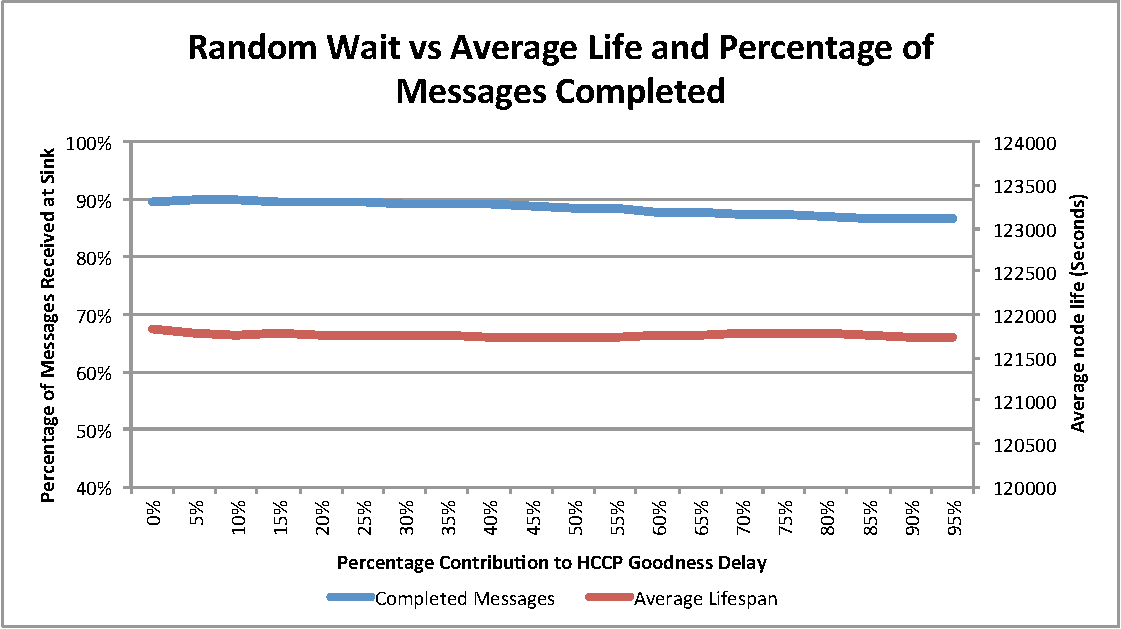
\includegraphics[width=0.9\textwidth]{images/simulation/goodness/Random3.pdf}
	\caption{The relationship between HCCP Goodness Delay using Random Wait Times and simulation results.}
	\label{fig:images_simulation_goodness_Random}
\end{figure}


Using Random as the
sole HCCP Goodness factor does not work well, as seen in Figure~\ref{fig:images_simulation_goodness_Random} Randomness
has very little effect on the network throughput or average node life. 
But Random works well paired with other factors 
as a tie-breaker, making one 
mote announce it's clusterhead status before a neighbouring node of similar
configuration. Using Randomness as a tie breaker works especially well early on in the
network's life, as many of the motes will have empty or nearly-empty messages queues and
full battery power. If two motes have the same Goodness Delay they will transmit their
candidacy or clusterhead announcement at the same time, potentially creating collisions
in the network.

\subsubsection{Effect of Sensor Mission on HCCP Goodness Delay}



Sensor mission is a percentage of how important the sensors are for a given mote. For instance,
a router mote with no sensors would have a sensor mission of 0\%, since it has no sensors. A
mote with very expensive sensors should almost never be a clusterhead, preserving its battery power
to collect more information. This value can be manually set, or automatically created by
counting the number of sensors that are being read and creating a Sensor Mission percentage from that
information.

\begin{figure}[tbhp]
	\centering
		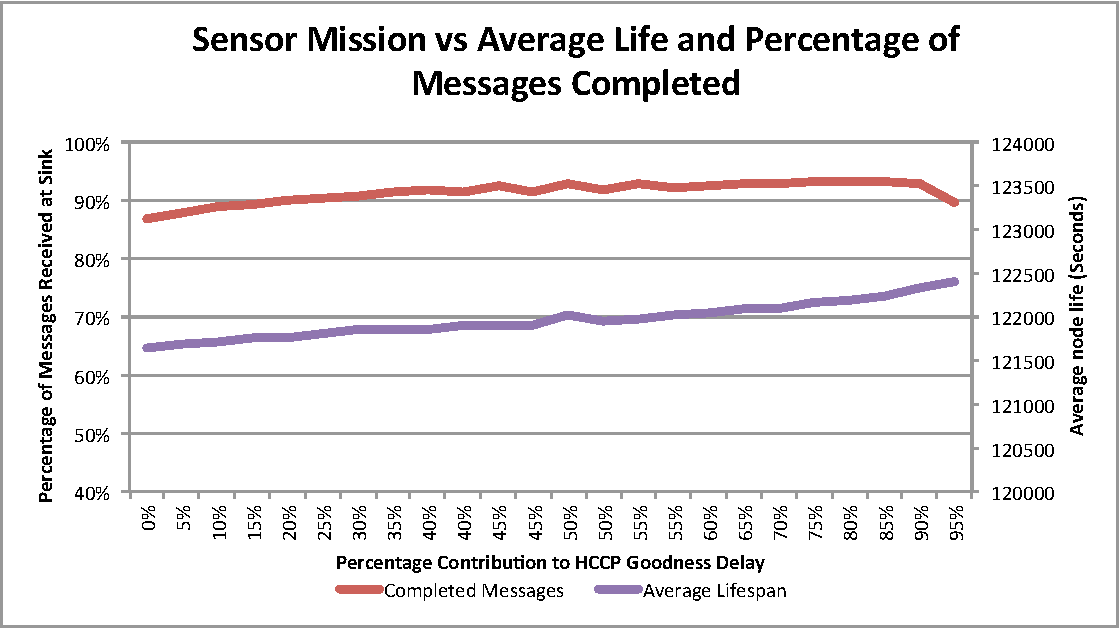
\includegraphics[width=0.9\textwidth]{images/simulation/goodness/Sensor2.pdf}
	\caption{The relationship between HCCP Goodness Delay using Sensor Mission and simulation results.}
	\label{fig:images_simulation_goodness_Sensor}
\end{figure}

Sensor mission creates a positive trend in both average node life and message throughput, as seen in 
Figure~\ref{fig:images_simulation_goodness_Sensor}. This
is because routers were given a sensor mission of 0 and sensor motes were given high Sensor Mission.
Providing motes with a Sensor Mission value is the best case as motes will then `know' how good
they are at the clusterhead task, making better router motes and motes with larger message queues
clusterhead motes more often. The problem with providing motes with Sensor Mission values is that
it is manual labour, and must be configured before the network is deployed. Also, Sensor Mission would 
be the most successful with a heterogeneous network; if all motes are the same and have the same Sensor
Mission, the clusterhead elections would degrade to an HCCP network that is 100\% focused on Random since all
motes would be generating the same Goodness Delay values.

%As discussed Section~\ref{simTuning}, he preset Sensor Mission is the ideal case for tuning a network to create long-lived
%networks. The results found in the simulation show that that preset Sensor Mission 

\subsubsection{Paired Factors in Heterogeneous Elections}
More than one factor can be paired together in the heterogeneous election to generate the Goodness
Delay. When networks first start, all message queues will be empty and all
batteries will be at 100\%, this will cause collisions during the 
HCCP Candidate Announcements, since all motes that elect to 
be a clusterhead that round will attempt to transmit their 
candidacy at about the same time (which will be close to immediately) if
the HCCP Goodness Delay is 100\% generated from a single factor. 
Adding a small percentage of the Random factor  will vary the 
generated transmission times, preventing the problem of equal Goodness Delays.

When adding Randomness to the Goodness Delay calculation will first
generate a goodness based on a primary factor (such as Available Message Queue Size or
Available Battery Power) which makes up the majority of the time, say 90\%. 
The Randomness will make a 10\% variance of the remaining time. 
The variance in the delay time will effectively be a tie-breaker for the transmission times
for the motes, avoiding many collisions while sending the announcements. The drawbacks to adding 
the Random factor to the Goodness Delay is that it adds no value to the Goodness Delay, as discussed
in Section~\ref{randomDelay}. Though, a small amount of Random Delay in the network 
is beneficial to the network due to the collisions it avoids. 


\subsection {Tuning HCCP for Power Efficiency}
\label{simTuning}
%lifespanCompare_higherfreq/comareLifespan.xlsx

\begin{figure}[htbp]
    \centering
        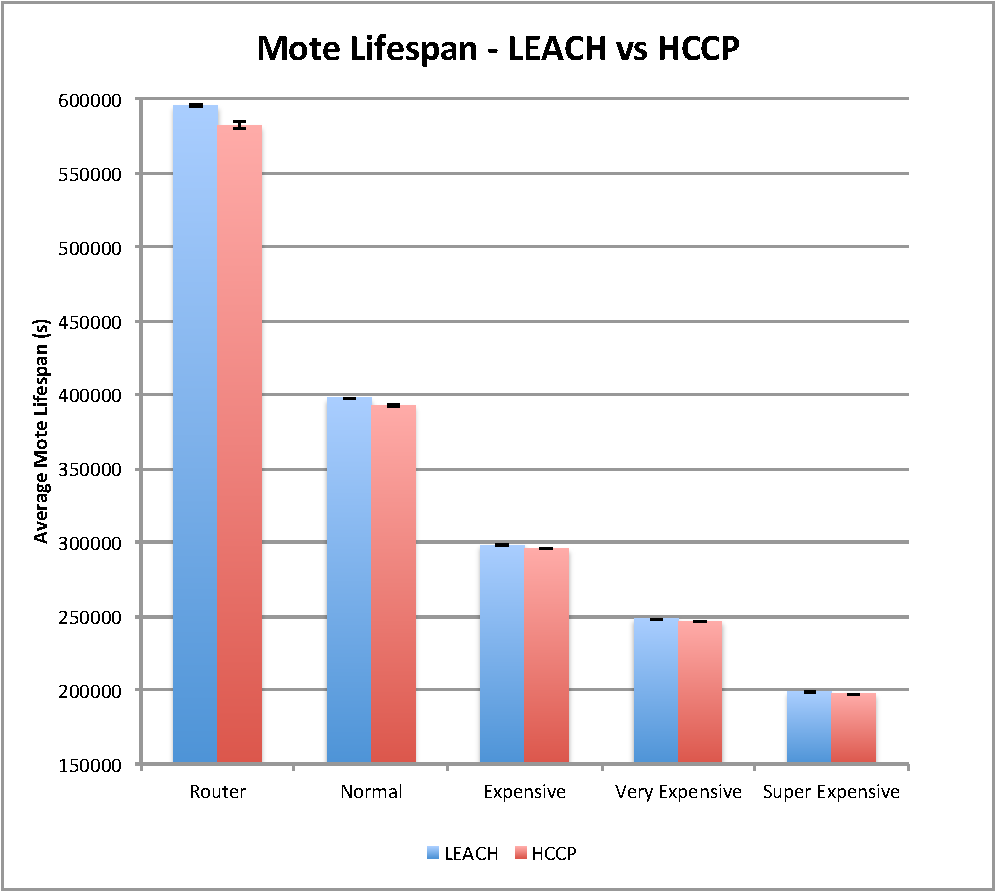
\includegraphics[height=3.5in]{images/lifespan/life.pdf}
    \caption{Tuning the efficiency of HCCP by minimizing Roundtable discussion allows HCCP to have networks lifespans approximately equal to LEACH.}
    \label{fig:images_lifespan_life}
\end{figure}

\begin{figure}[htbp]
    \centering
        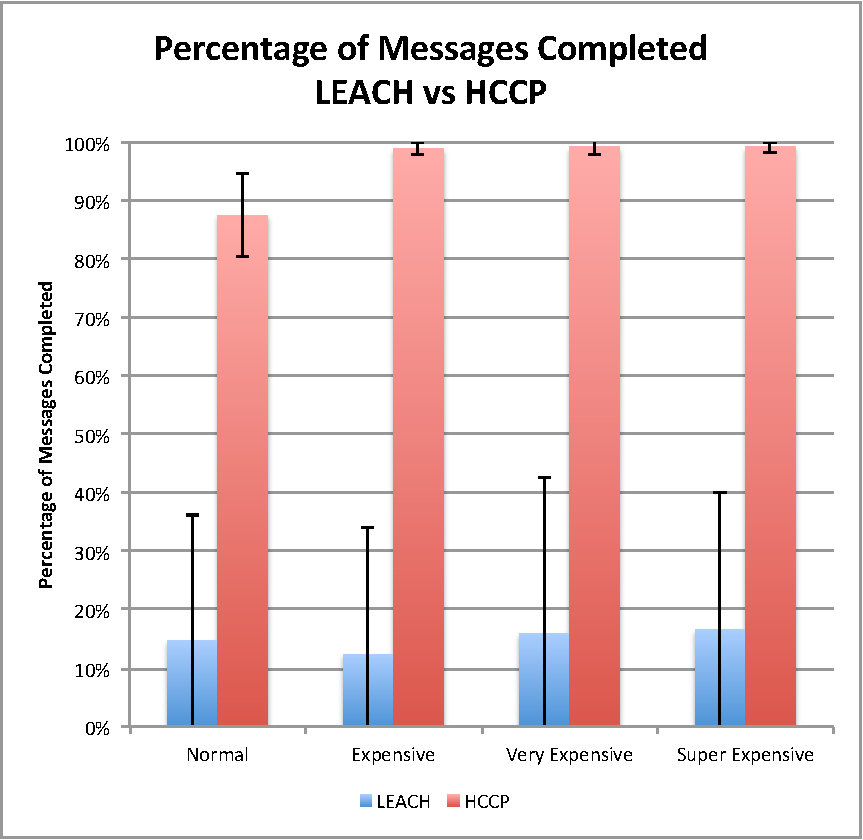
\includegraphics[height=3.5in]{images/lifespan/messages.pdf}
    \caption{In a tuned network, HCCP still has a much higher message throughput.}
    \label{fig:images_lifespan_messages}
\end{figure}

HCCP adds more time where all the motes are fully powered on than LEACH, because of the Roundtable Discussion 
and Clusterhead Candidacy stages. These extra steps cause an energy drain on the network,
but add lots of value to the network in terms of message throughput and data dissemination. 
As mentioned in Section~\ref{implementationTuning}, HCCP can be tweaked to be more power efficient while
still utilizing the gains from the Goodness Delay.

The easiest gain is to eliminate the Roundtable Discussion. This will improve network life, but decrease the 
ability to quickly disseminate information. For static networks that require a long lifespan, this is a good option.

The other option is to eliminate the Two-Stage Election, by eliminating the Clusterhead Candidacy stage. To compensate
for not having the Clusterhead Candidacy stage, the Clusterhead Election stage can be used to implement
the Goodness Delay features. To do this: in the Clusterhead Election, if a different mote announces itself
as a clusterhead first, concede being a clusterhead and become a clustermote. This is the same idea as used in Clusterhead Candidacy, but
done at the same time as a Clusterhead Election. The network will then choose slightly less optimal clusterheads, 
but overall creates a gain in which motes elect to be clusterheads. See Section~\ref{noCC} for more details about not using 
a Clusterhead Candidacy phase.

A well-tuned HCCP network will have a slightly shorter lifespan than a comparable LEACH network, but will have a
much higher message throughput than the LEACH network due to the quality of clusterheads that are chosen.
If lifespan is more desirable than message throughput, the Sleep period between 
election cycles could be extended to add lifespan to the network, which would make HCCP have a longer
lifespan for the same message throughput as LEACH.

A simulation was created with the HCCP and LEACH phases set to the same length. The results can 
be seen in Figures~\ref{fig:images_lifespan_life} and \ref{fig:images_lifespan_messages}.
LEACH has a longer lifespan, but dismal message throughput, while HCCP has
excellent message throughput. The lifespan of the router mote is noticeably lower in 
HCCP due to HCCP leveraging the router motes to be clusterheads more frequently, which 
in turn is increasing the message throughput. Consequently, the  router motes have 
shorter lifespans as the network relies on the routers to become clusterheads more frequently. 




\subsubsection{Eliminating the Clusterhead Candidacy Phase}
\label{noCC}
The Clusterhead Candidacy phase is a phase in HCCP that can be considered overhead, and 
is an obvious target to eliminate when looking to achieve longer lifespans. The Clusterhead
Candidacy phase offers very little in the way of overhead, however, since all motes that are not considering
being a clusterhead are sleeping during this phase. The clusterhead motes will then 
have time to share information about which motes should be clusterheads for that round. If the
Clusterhead Candidacy phase is dropped, the functionality must be moved to the Clusterhead Election phase.

The new Clusterhead Election phase would then work as follows: 
\begin{enumerate}
    \item Choose to be a clusterhead or not
    \item Listen for clusterhead elections. If clusterhead, use Goodness Delay to discover how long to wait until it is time to Announce itself as clusterhead.
    \begin{itemize}
        \item If a mote that has elected to be a clusterhead hears a clusterhead announcement before it sends one, choose to not be a clusterhead, and follow the mote that sent the clusterhead election.
    \end{itemize}
\end{enumerate}

%compareCCandNo_crazyHighFreq

\begin{figure}[htbp]
    \centering
        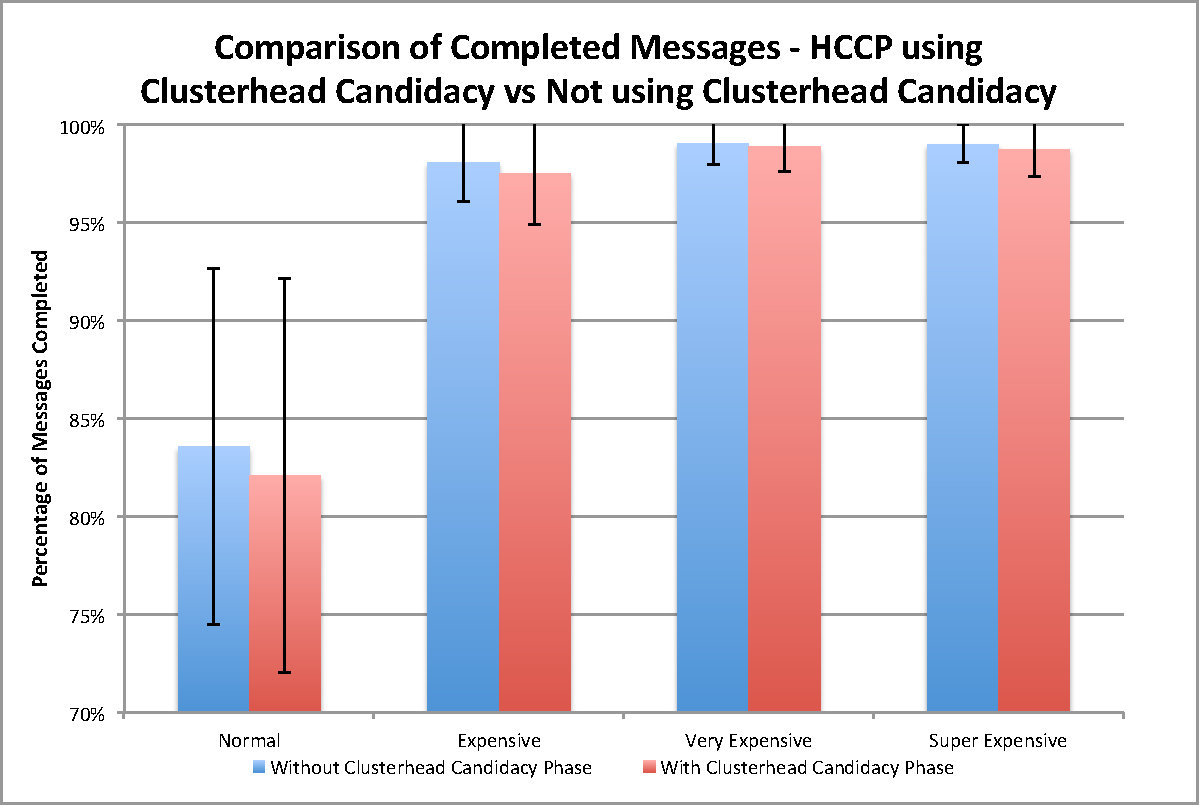
\includegraphics[height=2.9in]{images/ccVsNo/messages.pdf}
    \caption{ HCCP using Clusterhead Candidacy vs Not using Clusterhead Candidacy. The message throughput is comparable between the two networks.}
    \label{fig:images_ccVsNo_messages}
\end{figure}
\begin{figure}[htbp]
    \centering
        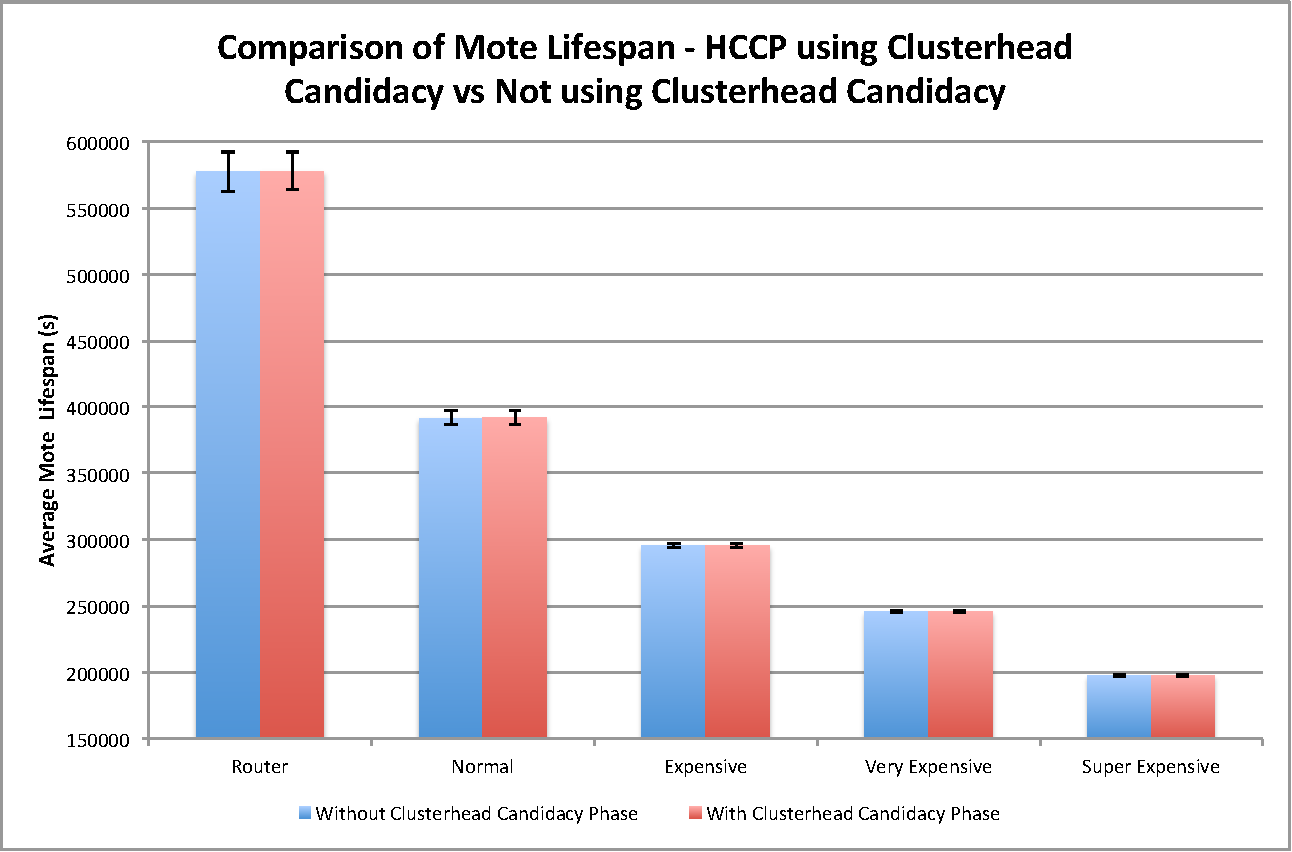
\includegraphics[height=3.1in]{images/ccVsNo/lifespan.pdf}
    \caption{HCCP using Clusterhead Candidacy vs Not using Clusterhead Candidacy. The results are quite even in terms of mote lifespan.}
    \label{fig:images_ccVsNo_lifespan}
\end{figure}


The rest of the protocol runs as previously prescribed. The problem with overloading the Clusterhead Announcement is that when
a collision occurs, it will cause much more damage to the entire cycle of the protocol. If a collision occurs during the 
Clusterhead Candidacy phase, one or both of the motes that are announcing their candidacy will opt to not be clusterheads, 
meaning that there will not be many collisions during the Clusterhead Announcement phase. When a collision happens in the
overloaded Clusterhead Announcement none of the motes in the neighbourhood will be able to follow either of the
motes that made the announcements, since the messages will be garbled. This means that the motes will continue listening for
clusterhead announcement messages, which means that these motes will at best be using the third best clusterhead mote in the neighbourhood (the next best
mote after the two motes that had a collision).

Two simulations were created with all parameters the same, with the exception that one of the simulations 
used a modified version of HCCP that dropped the Clusterhead Candidacy phase. The results, as seen
in Figures~\ref{fig:images_ccVsNo_lifespan} and \ref{fig:images_ccVsNo_messages}, show that whether the Clusterhead
Candidacy phase is independent, or merged into the Clusterhead Election phase the results are approximately 
the same. This means that though merging the Clusterhead Candidacy and Clusterhead Announcement phases saves
energy since motes are not on as long each cycle, clustermotes are using poorer clusterheads each round.
Based on the simulation results, 
there is very little difference between running HCCP in either of these configurations, so either could be used in 
a physical deployment. 




\subsubsection{Sink Sleep vs Suboptimal Clusterheads}

The HCCP Clusterhead Candidacy stage causes an issue called HCCP Blocking (previously discussed in 
Section~\ref{hccp_blocking}) where messages will not flow into 
motes that are in range of the sink. There are two methods of allowing messages to get into the
motes that are in radio range of the sink:
\begin{itemize}
    \item allow the sink to sleep some percentage of the time, or
    \item have suboptimal clusterheads which will elect to be clusterhead despite the fact there is a better clusterhead in the neighbourhood. 
\end{itemize}
There are drawbacks to both of these options. If the sink is asleep, no messages are being received at the sink, which could effect how
many messages reach the sink. If suboptimal clusterheads are used, more motes are electing to 
be clusterheads, more motes are clusterheads, which puts a larger drain on more motes.

Simulations were run to see which method is better for solving the HCCP Blocking problem. 
Simulations were run with 20 repetitions each, using the same starting seeds. 
Figure~\ref{fig:images_SleepVsNo_Messages} shows that there were no real differences with 
the percentage of messages received at the sink. This means that even if the sink sleeps
every few rounds, there is no effect to the throughput of the network. This makes 
sense, as messages must flow into the motes adjacent to the sink before they can be 
hopped into the sink. Whether the sink sleeps, or motes elect to be 
suboptimal clusterheads, the path taken will be approximately the same. Note that 
router motes in the simulation did not make messages, and are therefore left off the chart.

There is also a concern that if the suboptimal clusterhead option is chosen, then 
the lifespan of the network might be lessened, since more motes will be clusterheads
at the same time. Figure~\ref{fig:images_SleepVsNo_MoteLife} shows us that 
the there is no significant hit to the network life. While difficult to see in the chart, there 
is no statistical difference between the two options for the `Super Expensive' motes 
(196734 $\pm$ 611 for Sink Sleep Super Expensive motes, 196782 $\pm$ 624 for Suboptimal
Super Expensive motes). 
%Data from Charts/SleepVsNo

There were also no significant differences between the two methods in terms of 
number of collisions in the network. This is also interesting since 
suboptimal clusterheads means that there will be more traffic in more areas, clusterheads
will be closer to one another.

\label{sleepVSsubop}
\begin{figure}[htbp]
    \centering
        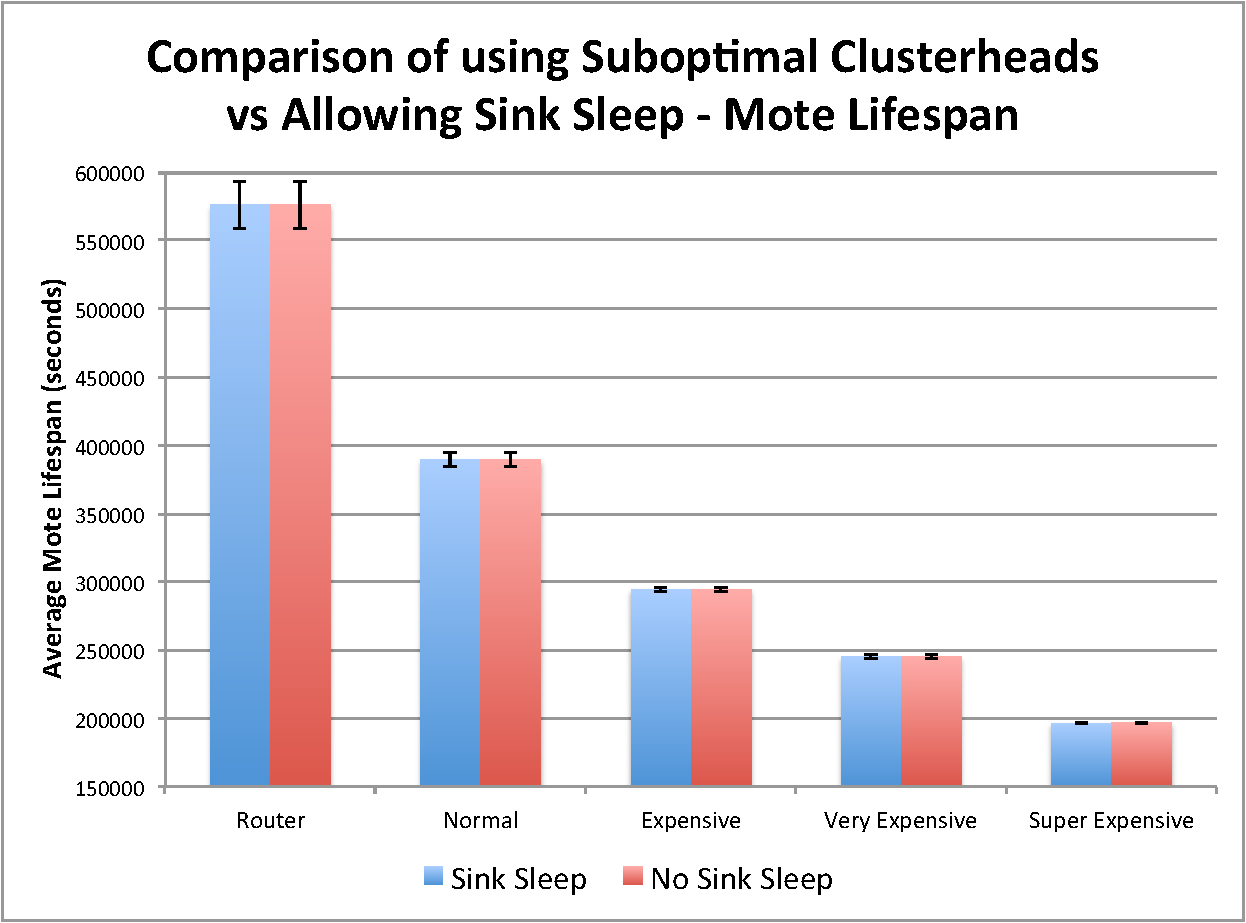
\includegraphics[height=3.2in]{images/SleepVsNo/Messages.pdf}
    \caption{The percentage of messages created that were received at the sink is approximately the same whether the sink periodically sleeps or not.}
    \label{fig:images_SleepVsNo_Messages}
\end{figure}

\begin{figure}[htbp]
    \centering
        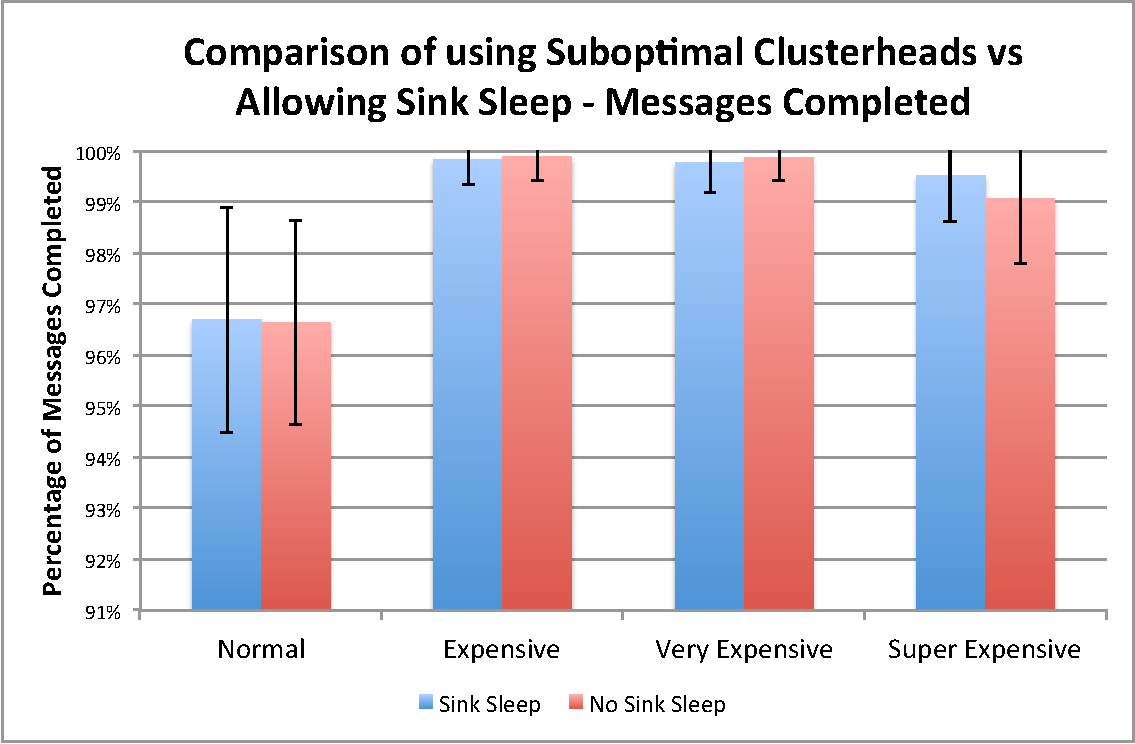
\includegraphics[height=3.2in]{images/SleepVsNo/MoteLife.pdf}
    \caption{Average mote lifespan is unaffected by whether the sink periodically sleeps or not.}
    \label{fig:images_SleepVsNo_MoteLife}
\end{figure}

\subsubsection{Clusterhead Opt-out}
As discussed in Section~\ref{optout}, if a network is set up to do multiple iterations of 
the TDMA schedule, clusterheads should be able to opt out during the Roundtable 
Discussion.
After running some test simulations to show that this could be a successful 
idea, contradictions in the concept were found which showed how the idea is 
flawed.
To successfully have a long-lived network, the Roundtable Discussion 
should be as short as possible, or left out altogether as the whole
network must be on for the stage to be fully utilized. Since Clusterhead Opt-out
requires Roundtable Discussion, its not a good fit for long-lived networks. In
general, it would be better to have one longer TDMA run schedule than a
repeated TDMA schedule. A longer TDMA schedule run allows the network to send as many 
messages as possible, and even allows motes to turn off when they are out of messages, and turn
back on and send more (provided it is still the mote's TDMA timeslice and the mote has
more messages ready to send).
Conversely, repeated TDMA schedules keep the same clusterhead, putting a large
load onto one clusterhead and losing a large amount of network adaptivity. Another 
drawback is throughput. Since one mote remains a clusterhead for an extended period of time, 
it can't send the messages it's collecting to motes closer to the sink. This causes the
messages are hopped much slower, causing message queues to fill.

There are instances where  Clusterhead Opt-out could still be useful, such as
networks that require quite long lifespans, where motes may go temporarily offline
or die at a frequent rate. The one election with many TDMA schedules would
allow the motes to send in their readings if and when they can. If one large
TMDA schedule is run and missed, motes will not be able to send in their readings
since they may be dead by the time the next large TDMA schedule is published.
This is, unfortunately, quite difficult to show in simulation, but presented 
as a possible niche case where Clusterhead Opt-out could still be useful.


\subsubsection{Automated Ad Hoc Backbone with HCCP}
There has been research into two-tier networks and networks with a backbone set of motes that are
set in the network for routing messages. LEACH does not take advantage of 
the benefits offered by these motes, as it does not consider the heterogeneity in the network. Heinzelman et al.~\cite{leach}
mention that a two-tier network could be created where the routing motes collect from the neighbourhood motes,
then run a LEACH schedule across the routing motes where \emph{only} the 
routing motes handle routing the messages to the sink.
The problem that exists with this model is that if the backbone gets broken,
there is no way for the network to recover, as shown in Figure~\ref{fig:images_BrokenBackbone_Backbone} (note that the sink is 
not visible in the figure). 
No motes past the break in the backbone will be
be able to send messages to the sink.

\begin{figure}[tbp]
    \centering
        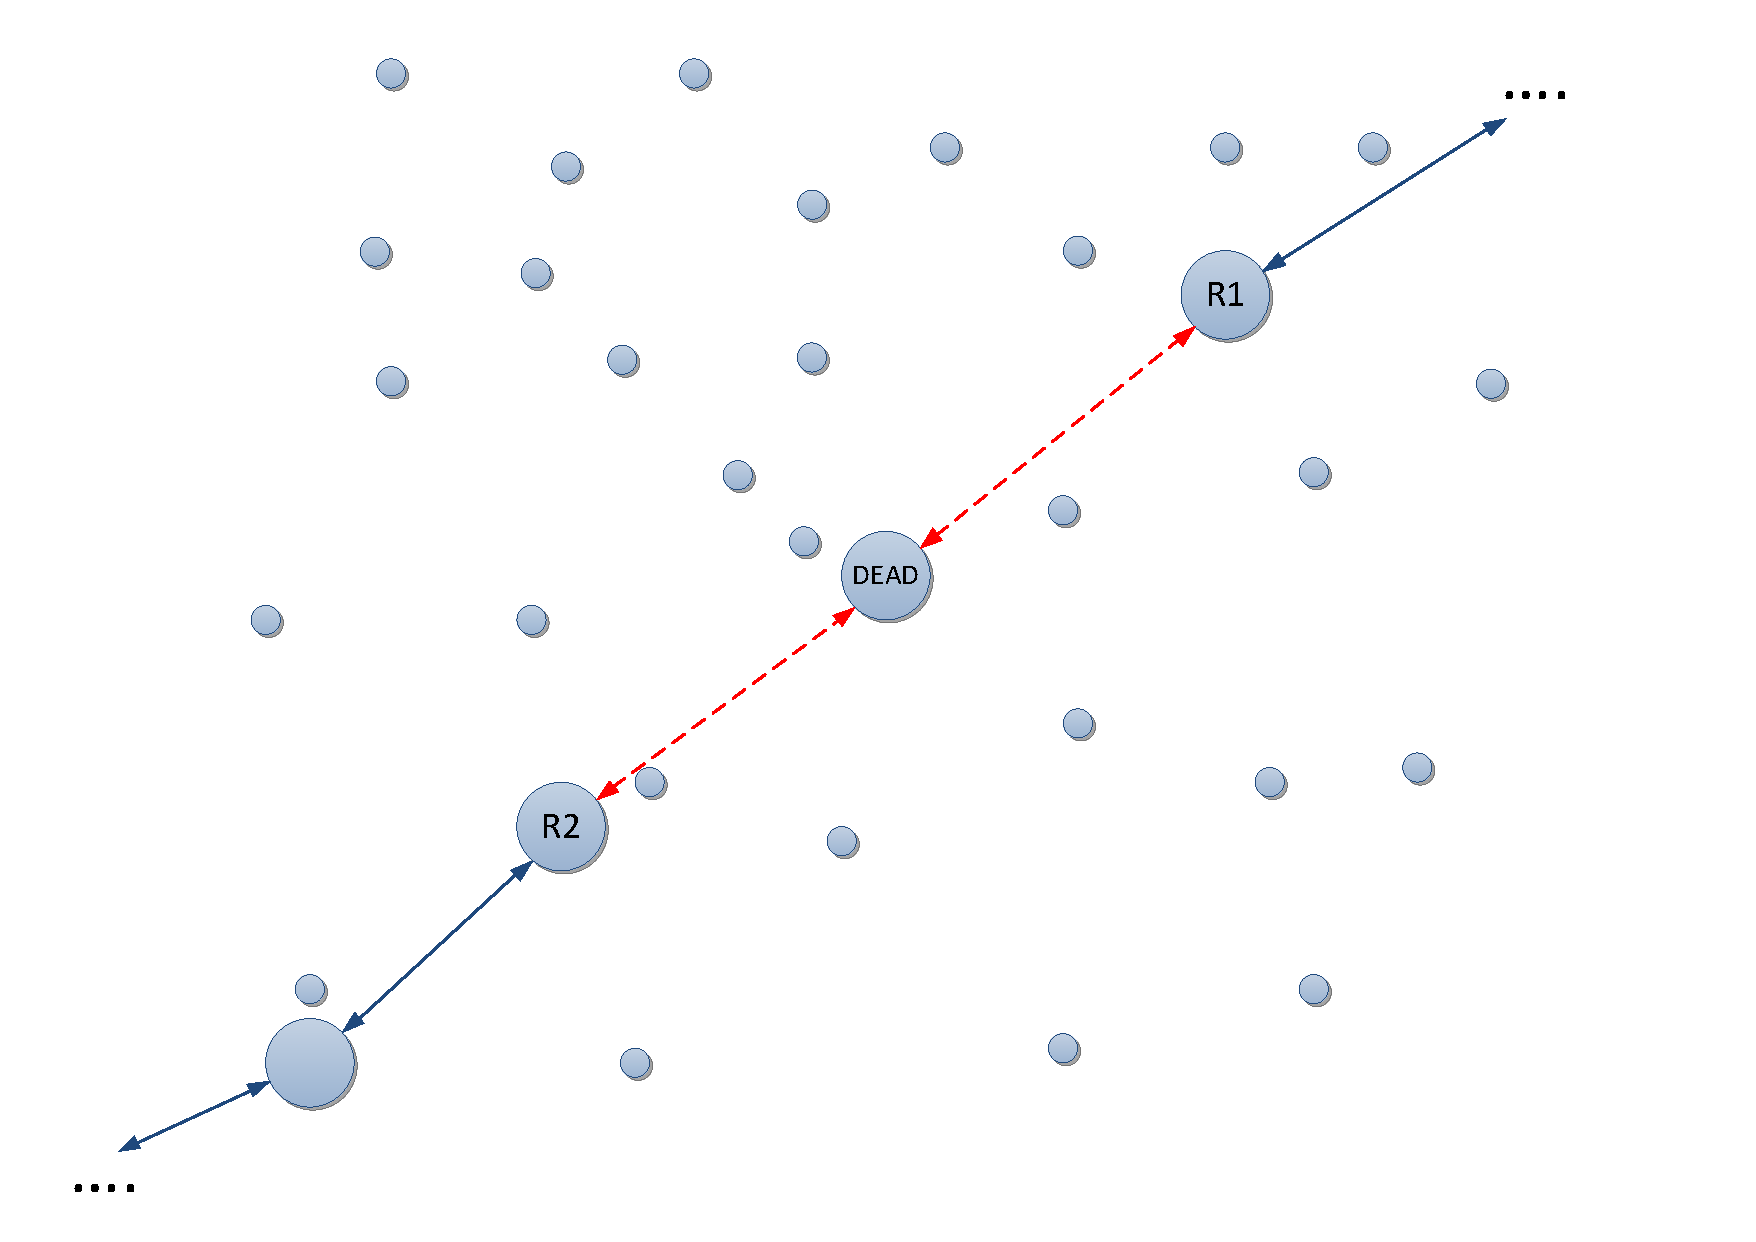
\includegraphics[width=6.5in]{images/BrokenBackbone/Backbone.pdf}
    \caption{Snapshot of a part of a WSN: routing mote R1 can not communicate with routing mote R2 because the routing backbone is broken.}
    \label{fig:images_BrokenBackbone_Backbone}
\end{figure}


HCCP uses LEACH as a starting point, but eliminates this problem by 
distributing the clusterhead task to all motes in the network. HCCP will ensure that
motes which are better at the clusterhead task will choose to be a clusterhead more often 
than motes which are not as good at the clusterhead task. This is due to the Goodness Delay that
is part of the clusterhead election. Motes with larger message queues, or more battery power,
or that have been given a low Sensor Mission value will choose to be clusterhead motes more often.
Due to this, motes that are not good clusterheads will not choose to be clusterheads,
and motes that are good clusterheads will choose to be clusterheads. This will create an 
ad hoc backbone across the motes which are inclined to be clusterheads. But, if the backbone is broken
by a mote dying or going offline, the messages from beyond the break can still move past the break. This
is because all motes can assume the clusterhead role. If there is no router mote in an area (due to the 
router mote going offline, or poor network distribution), other motes in the network will take on the 
clusterhead role. This will cause the motes that are non-router motes to die sooner, but 
keep the messages from the network flowing through areas with no router motes.

The HCCP Goodness Delay creates more robust networks that can 
handle change within the network with minimal negative effects to 
the network. Messages will still be routed well due to the 
Roundtable Discussion sharing routing information, and 
messages can move  over breaks in backbones since all motes can be assigned the clusterhead task.


%\textbf{Implement `failing' as a clusterhead. HCCP will recover, LEACH will not. -- add if there is time}
%This will need repeated schedules to work well. The runtime is now runtime/NumRepeats to keep the leach/hccp comparison 
%pretty consistent.
%\textbf{Movement... ugh. This would put the silver bullet in LEACH, but is hard to approach. - add if there is time}


\section{Testbed Setup, Deployment and Results}
\label{ch:Physical Network}

To show the gains of leveraging heterogeneity in WSNs, a testbed deployment was created and run. Test runs
using both HCCP and LEACH as the network clustering protocol were created, run and compared. 

\subsection{Building HCCP with 802.15.4}


The goal of HCCP is to intelligently cluster motes in Wireless Sensor Networks, not to 
create a new wireless standard. HCCP works as a middleware layer between the 
mote's application and the wireless radio that is using some wireless protocol, 
such as Bluetooth, ANT radios, or even WIFI (802.11). The
network protocol used in the testbed deployment was 802.15.4.

Building on top of 802.15.4 requires that the protocol's requirements are met. 
A basic packet in 802.15.4 is constructed using several segments that
have information in well-defined places, as seen in Table~\ref{fig:eightOhTwo}.
The physical layer header preamble is handled by the hardware and is outside the scope
of this work. It is assumed that the preamble is functioning properly, and no changes need to be made
to it for the support of HCCP.

The bytes following the physical layer preamble are the Media Access Control (MAC) layer
header bytes. The bytes in the header are well-defined by the 802.15.4 protocol,
with each byte given a special meaning in the header.  
The first two bytes are the Frame Control Field (FCF), which can be seen in Table~\ref{fig:eightOhTwo},
that tell the packet parser
what to expect in the rest of the packet. The FCF details values which affect
how long the packet header will be such as whether
the security is enabled, and which type of MAC addresses the packet header
contains. 

The next byte is the packet sequence number, which is a value that gets incremented for
every packet the sending mote sends. It is used to recreate data that is split across multiple packets
that are being sent to the receiving mote. In the testbed deployment, data is assumed to be 
contained within one packet. The sequence number of the packets is therefore irrelevant, but can not be
left out without violating the guidelines described by the 802.15.4 standard.


%\begin{figure}[htbp]
%	\centering
%		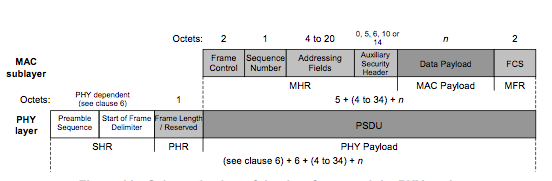
\includegraphics[width=6.5in]{images/protocol/8oh2.png}
%	\caption{Breakdown of data packets in 802.15.4.~\cite{zigbee}}
%	\label{fig:eightOhTwo}
%\end{figure}
%\begin{figure}[htbp]
%	\centering
%		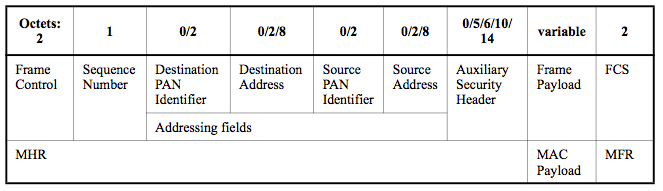
\includegraphics[width=5in]{images/protocol/MacFrame.png}
%	\caption{General 802.15.4 frames, as shown in the 802.15.4 standards document~\cite{zigbee}.}
%	\label{fig:images_protocol_MacFrame}
%\end{figure}


\begin{table}[ht]
	\centering
	\begin{scriptsizetabular}{|c|c|c|c|c|c|c|}

      \hline 
      Octets:  &          &           &              &          &        &  \\
      variable & 2        &  1        & 4-20         &  0-14    & n      &  2\\
      \hline 
      Preamable & Frame    & Sequence  & Addressing  & Security & Data   &  Checksum\\
      Sequence & Control  & Number    & Fields      & Header   & Payload &  \\ 
      \hline
    \end{scriptsizetabular}
    \caption{Breakdown of data packets in 802.15.4. Adapted from~\cite{zigbee}.}
    \label{fig:eightOhTwo}
\end{table}


% m{width}
%\begin{table}[ht]
%	\centering
%	\begin{scriptsizetabular}{|c|c|c|c|c|c|c|c|}
%		\hline
%		Frame  & Sequence & Destination & Source & Auxiliary & HCCP Packet & HCCP Packet & Checksum  \\
%		Control  & Number & Address & Address & Security Header & Type & Payload &  \\
%		\hline 
%	\end{scriptsizetabular}
%	\caption{Customized 802.15.4 packets for use in HCCP with more detail.}
%	\label{tab:Mypackets}
%\end{table}
\begin{table}[ht]
	\centering
	\begin{scriptsizetabular}{|m{1cm}|m{1.35cm}|m{1.75cm}|m{1.35cm}|m{1.5cm}|m{1.25cm}|m{1.80cm}|m{1.5cm}|}
		\hline
		Frame Control & Sequence Number & Destination Address & Source Address & Auxiliary Security Header & HCCP Packet Type & HCCP Packet Payload & Checksum  \\
		\hline 
	\end{scriptsizetabular}
	\caption{Customized 802.15.4 packets for use in HCCP with more detail.}
	\label{tab:Mypackets}
\end{table}




Following the sequence number is the addressing field, which can be 4-20 bytes. The range is due to the 
way that 802.15.4 addresses can be specified. 802.15.4 has 20 byte addresses that are designed to be globally unique identifiers,
but can also use 4 byte addresses to create lightweight packets. When using the 4 byte addresses there is a good chance that 
two motes in the network could have the same address. This causes the tradeoff of reliability and understandably of data versus
the per packet cost to send a message in the network. There is both a source and destination address specified in the addressing field.

An optional security field follows the sequence number. This field could be used to encrypt the data in the packet,
but it not used in the testbed deployment. HCCP can be used with encryption using this field with little or no modifications
to the HCCP protocol.

Finally, the data payload for an 804.15.4 packet is where all the HCCP logic is added. HCCP divides up the 
data section of the packet into more well-known fields, much like the creators of 802.15.4 have done. 
HCCP divides the data section in to 8 bits for packet type, and the remainder is the packet data.
The custom HCCP packet format is shown in Table~\ref{tab:Mypackets}.  The
The HCCP values for the HCCP Packet Type field are as follows:

\begin{enumerate}
	\item \textbf{Clusterhead Candidacy Announcement} - {\tt 0x0} - The sender of this message is going to be a clusterhead candidate.
	\item \textbf{Clusterhead Announcements} - {\tt 0x1} - The sender of this message is a clusterhead. Following the HCCP header is the mote's ID.
	\item \textbf{Join Cluster} - {\tt 0x2} - The sender of this message wants to join the cluster of the recipient. The mote that has the address in the addressing field is the mote 
	it will follow. The clusterhead that is the recipient will use the `from' address as the ID of its new clustermote.
	\item \textbf{TDMA Schedule} - {\tt 0x3} - A broadcast message to all surrounding motes with the TDMA schedule the 
	clustermotes will be following. A sample TDMA schedule
	can be seen in Table~\ref{tab:tdma}. \begin{table}[ht]
		\centering
		\begin{tabular}{|c|c|c|c|c|c|c|c|}
			\hline
			Packet  &  Runtime for  & First ID & Second ID &  ... & nth ID\\
			Type &  each Mote (s or ms) & \& Delay & \& Delay &  & \& Delay \\
			\hline
			{\tt 0x3} & 20 & 12:20 & 18:40 & ... & 88:70\\
			\hline
		\end{tabular}
		\caption{Sample TDMA schedule as sent by the clusterhead to its clustermotes.}
	\label{tab:tdma}
\end{table}
	
	\item \textbf{Data Packet} - {\tt 0x4} - Messages sent from clustermotes to their clusterhead. $n$ data bytes will follow the type field.
	\item \textbf{Roundtable Discussion Packet} - There are a few well-defined packets that can be sent during a Roundtable Discussion. To save in the packets, they 
	can share the type field with the other well-defined packets, or can be assigned type values of their own.
	\begin{enumerate}
		\item \textbf{Clusterhead Opt-out} - {\tt 0x5} - Clusterhead can quit if there are multiple iterations of the 
		HCCP schedule. 
		\item \textbf{Roundtable Clusterhead Announcement} - {\tt 0x6} - a replacement clusterhead if an existing clusterhead opts out.
	\end{enumerate}
	\item \textbf{Other} - {\tt 0x8} - If any packets are defined for a customization of HCCP, this value can be used. An instance where other packets could be used
	is during the Roundtable Discussion, if the motes need to share some other information. In the testbed deployment, routing information is shared using the
	other packet type during the Roundtable Discussion time. The contents following the HCCP header are at the discretion of the network administrator.
\end{enumerate}

After the HCCP packet type field is the HCCP packet data field which contains the 
packet payload. After that the 802.15.4 checksum follows to make the packet 802.15.4 compliant.



\subsection{Description of Testbed Motes}
\label{ch:motes}

To create a heterogeneous WSN, motes from multiple vendors 
were selected for the experimental WSNs. The motes selected 
have different radios, run different operating systems and
have differing capabilities. Below is a description of the
motes used for the experiments, the capabilities of the motes,
the modifications that could be possible to increase heterogeneity and the modifications made to them.


\subsubsection {Sun Microsystems SunSPOT}
 
	Sun Microsystems Labs~\cite{sunspot} saw the need for easily programmable
	motes with solid form-factor and simple tools to use. 
	SunSPOT stands for `Sun Microsystems Small Programmable Object Technology', which 
	is designed to be simple to both program and deploy.
	Sun had already 
	created a version of Java to run on mobile phones called Java 2 Micro Edition (J2ME)~\cite{j2me}.
	Sun used this code base for a starting point for the SunSPOT programming interface. 


	The SunSPOTs are sold in boxes with 2 motes called ``free-range'' motes seen in Figure~\ref{fig:images_motes_sunspot1}, and 
	one base station mote, as seen in Figure~\ref{fig:images_motes_sunspotandBS}. The free range motes are complete with a 
	rechargeable battery
	that charges from USB, a CC2420 radio, a number of sensors and LEDs for the programmer
	to use. The free range SunSPOTs are divided into 2 boards, as seen in Figure~\ref{fig:images_motes_sunspot2}. The top board is the board visible
	on the top of the SunSPOT, which is the sensor board that holds all the 
	sensors, buttons and LEDS. The second board is the main board that hosts the microcontroller and the radio.
	The base station SunSPOTs share the same main board as the free range SunSPOTs, but do not have
	a rechargeable battery or a sensor board. The common main board is convenient, as the radio code
	can be shared between the both the free-range motes, and the base station.
	
	 \begin{figure}[htbp]
	 	\centering
	 		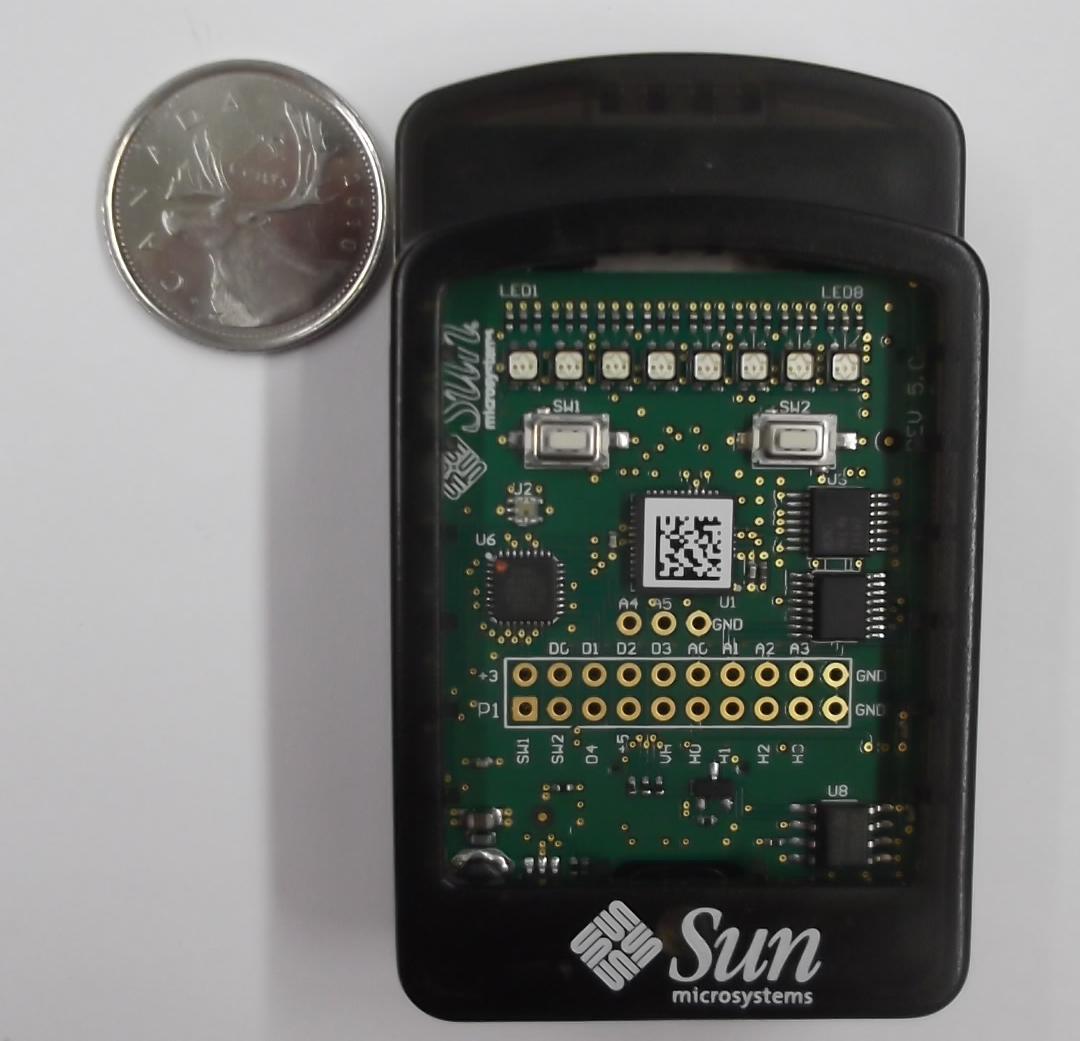
\includegraphics[height=3in]{images/motes/sunspot1.jpg}
	 	\caption{The Sun Microsystems SunSPOT.}
	 	\label{fig:images_motes_sunspot1}
	 \end{figure}
	\begin{figure}[htbp]
	 	\centering
	 		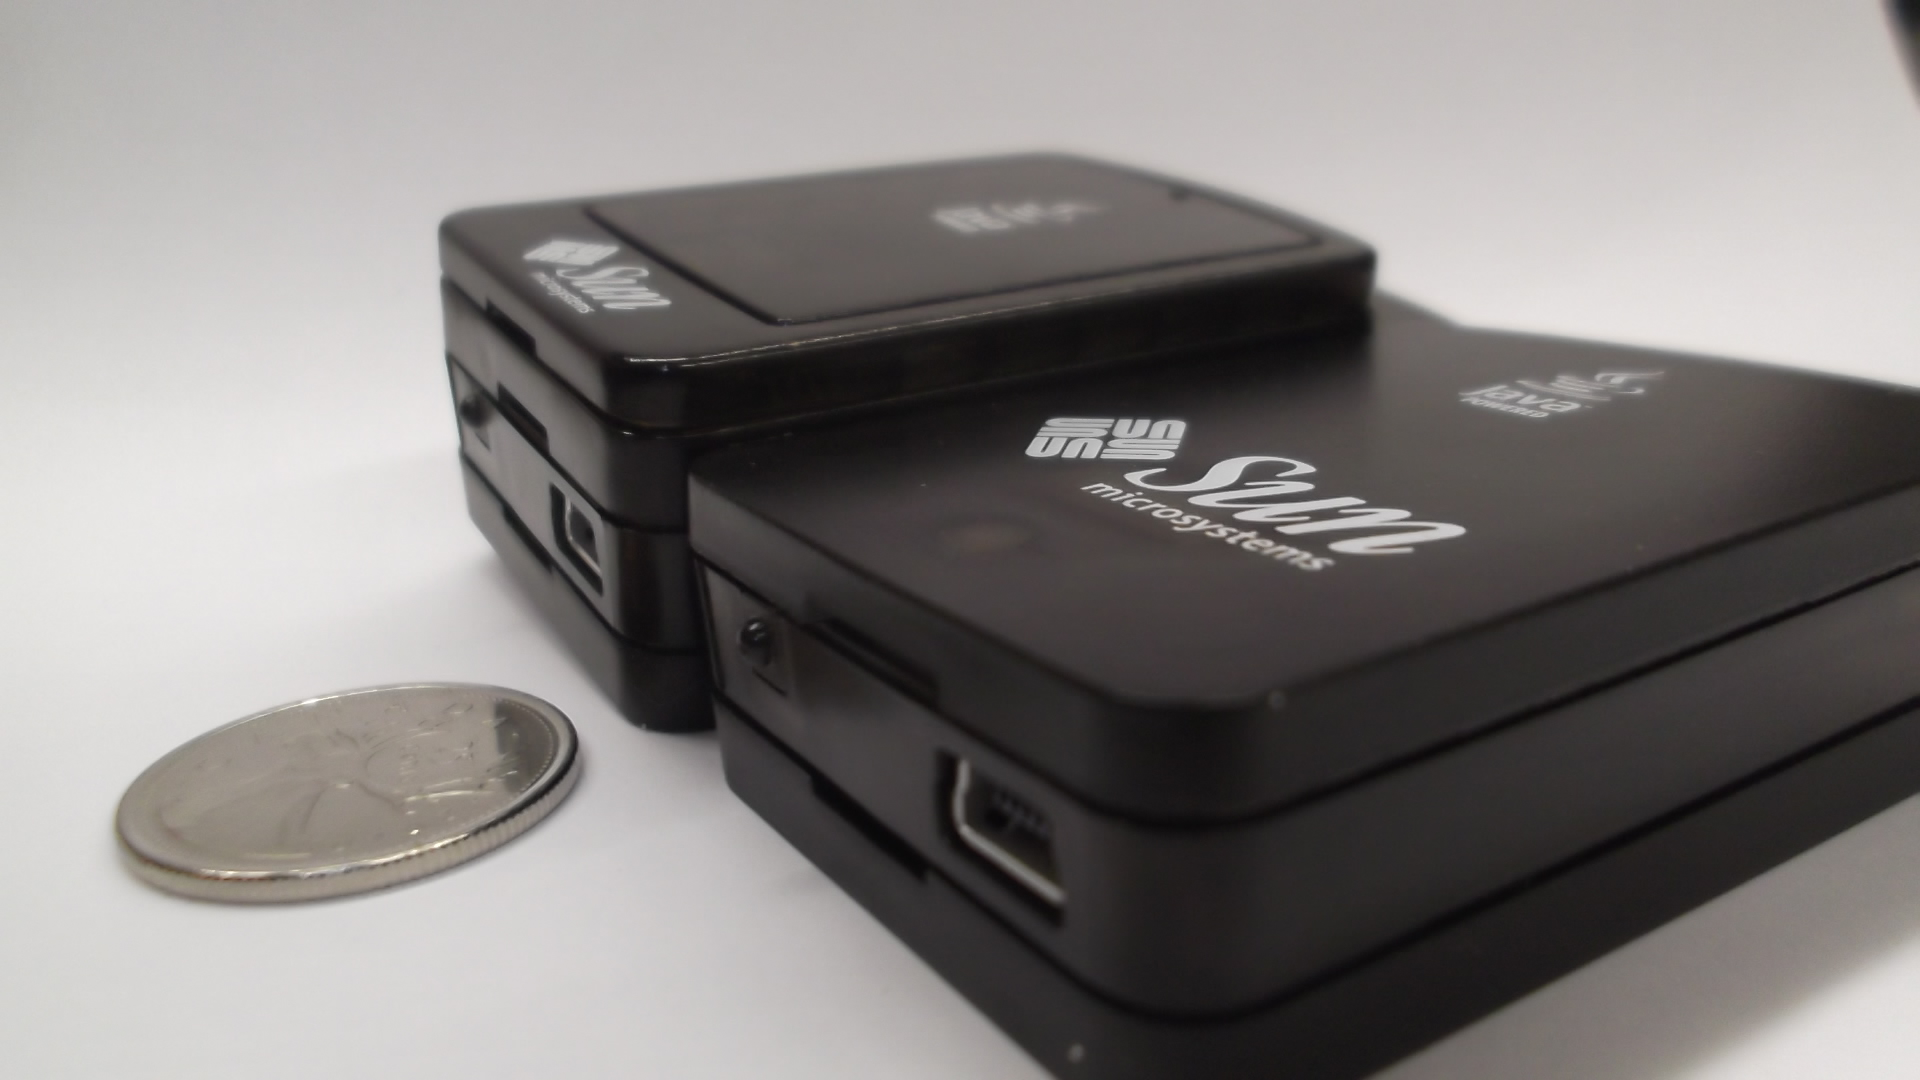
\includegraphics[height=3in]{images/motes/spotBSandMote.jpg}
	 	\caption{A SunSPOT free-range mote and SunSPOT base station.}
	 	\label{fig:images_motes_sunspotandBS}
	 \end{figure}
	 \begin{figure}[htbp]
	 	\centering
	 		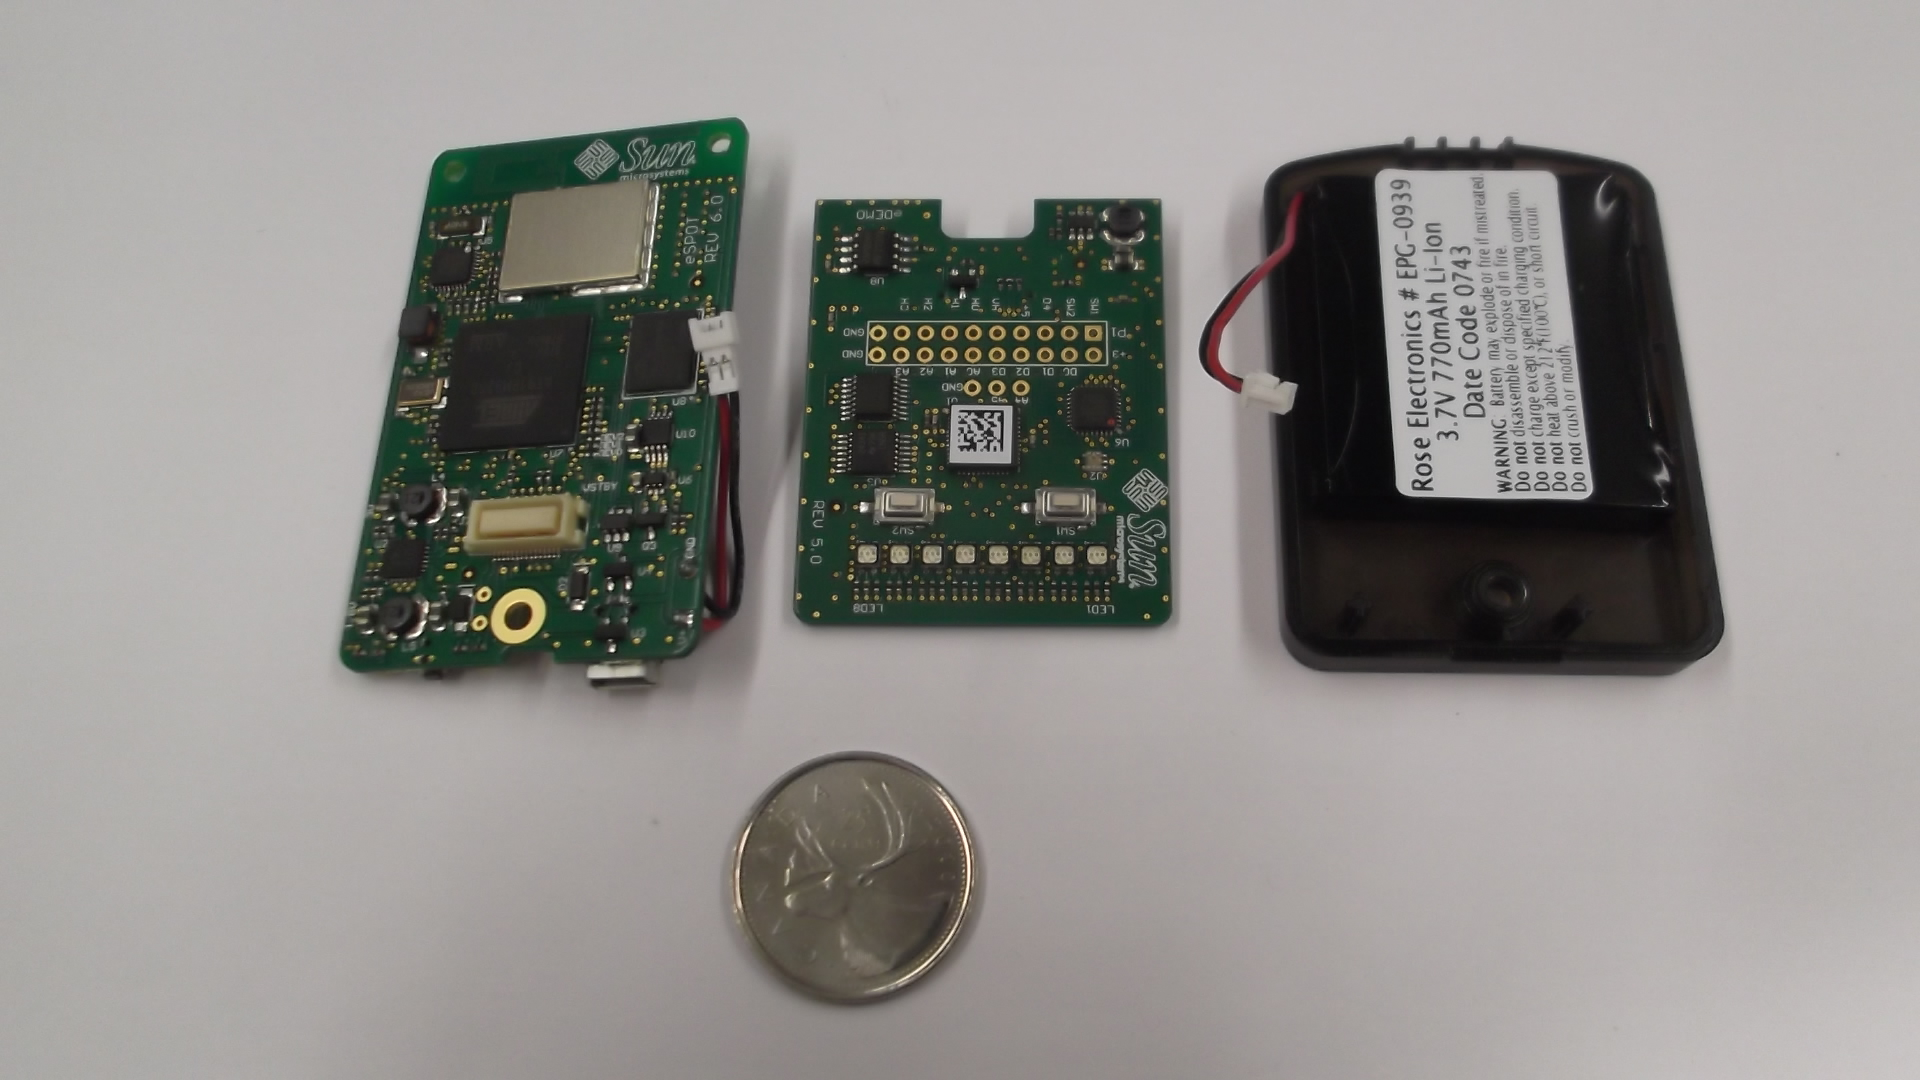
\includegraphics[height=3in]{images/motes/sunspot2.jpg}
	 	\caption{A SunSPOT taken apart to view the components in the casing.}
	 	\label{fig:images_motes_sunspot2}
	 \end{figure}
 
\paragraph{\emph{Possible Modifications to the SunSPOTs.}}
	The rechargeable battery the SunSPOTs ship with is small and does not hold 
	enough energy to power the SunSPOT for a long period of time. A simple modification is
	to remove the back of the SunSPOT, replacing the battery with any other power source providing 
	up to 4.9 volts as stated in the SunSPOT developer's manual~\cite{sunspotmanual}. 
	This could be done with 3 AA batteries, which would provide much more available energy.
	
\paragraph{\emph{Uses for the SunSPOT in a Heterogeneous WSN.}}
	The base station the SunSPOTs ship with makes a very convenient base station for a 
	WSN. The radio code developed for the free range SunSPOTs can be used on the base station
	while it is connected to a computer. The base station is designed to run with
	Java code developed using the SunSPOT suite developed for the SunSPOT, and
	the base station can be easily accessed via a Java program. The program running the 
	base station can then log the data to a database, or post it to a website to make the 
	data collected by the WSN available world-wide immediately.
	
	The base station could also be used to make an entire computer a mote.
	That is to say, the base station could be connected to a computer but not act 
	as a sink. This would allow the mote to have nearly unlimited power and memory resources, 
	making it an ideal routing mote.

	\begin{figure}[tbh]
		\centering
			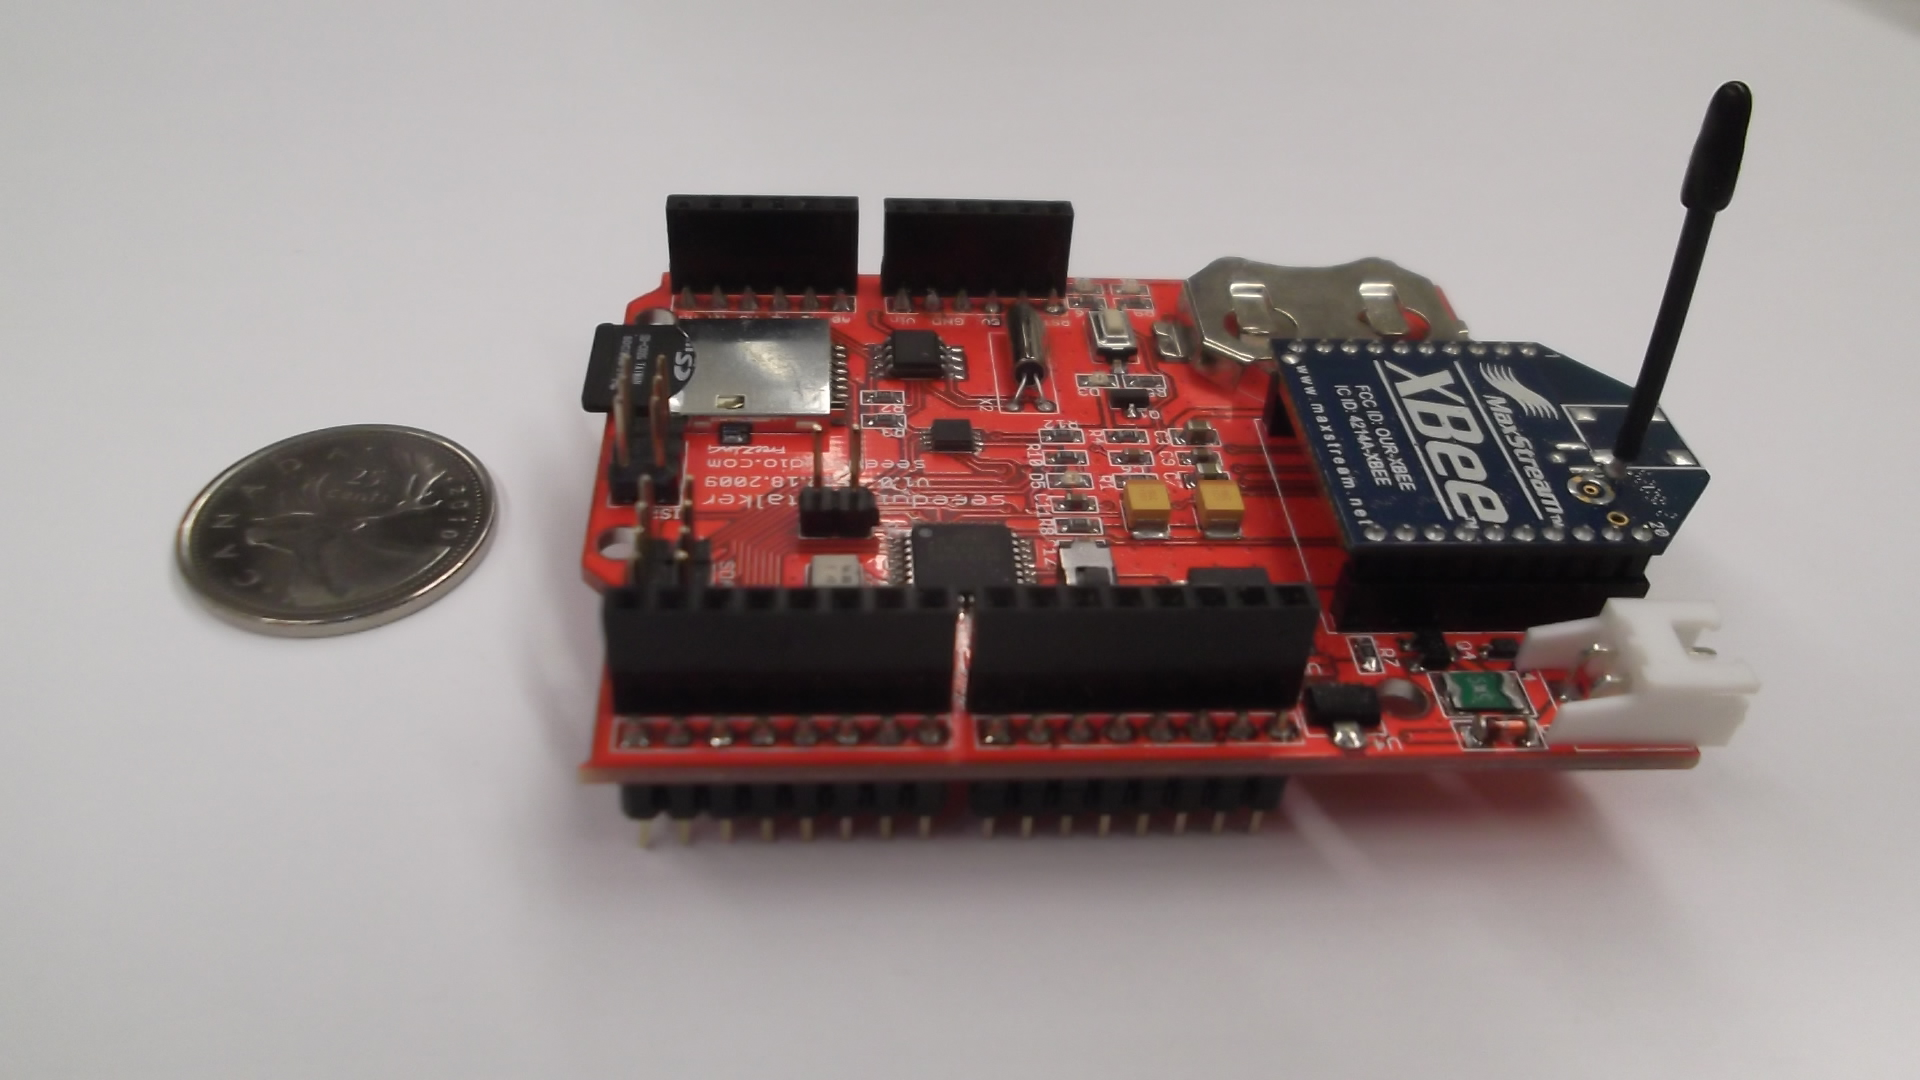
\includegraphics[height=3in]{images/motes/stalkerXbee1.jpg}
		\caption{Seeeduino Stalker with XBee port exposed.}
		\label{fig:images_motes_stalkerXbee1}
	\end{figure}

\subsubsection {Seeeduino Stalker and Arduino Technology}
	Seeed Studios~\cite{seedstalker} is a developer and retailer of microcontrollers online, 
	specializing in Arduino-compatible microcontrollers. One of the products they provide
	is a mote called the Seeeduino Stalker. The Stalker is a microcontroller based on the 
	Arduino design~\cite{arduino}, using a compatible processor and standard Arduino pin layouts.
	As seen in Figure~\ref{fig:images_motes_stalkerXbee1} the
	Stalker has an onboard battery, and logging capabilities, using MicroSD cards to log to.
	The Stalker does not ship with a built-in radio, but makes an XBee compatible slot available. 
	To allow the Stalker to communicate with the other motes, we chose the XBee Series 1 
	modules - which communicate using the 802.15.4 standard~\cite{zigbee}.
	
	The Stalker does not have any native sensing abilities, but can be configured to use
	either Arduino-compatible shields (which attach to the female pin headers on the board 
	to provide some service). This makes the Stalker ideal for creating highly customized
	motes. The Stalker could be configured to have no sensors to make a low-power routing
	mote with the ability to log large amounts of data on its MicroSD card. Or, can be configured
	to use a variety of sensors and be a specialized sensor mote.
	
	A problem does arise with the Stalker's battery power. The Stalker is sold with a port to 
	use a `button battery', as seen in Figure~\ref{fig:images_motes_stalkerXbee1}. More power is 
	very desirable, so the Seeeduino Stalker motes will need to be fitted with a larger battery supply before
	it could be used as a useful mote.  The Stalker is sold with a port to plug in an external 
	power supply, so this is not a large problem.
	
	A major problem with the Stalker is the CPU it uses. The CPU has very limited program space. 
	The code developed frequently overran the size of the program space, causing the 
	mote to crash. Due to this, a minimal installation of Contiki OS has been created to 
	allow the Stalker to work in the network with limited capabilities. The Stalker
	can only participate in the network as a clustermote, not as a Clusterhead.
	
	Another Arduino mote was made for the network. The Arduino Duemilanove is a more powerful Arduino with 
	more memory and fewer built-on features. The Duemilanove required an extension called 
	a shield to allow the board to use a radio, as seen in Figures~\ref{fig:images_motes_arduinoUnstack} 
	and~\ref{fig:images_motes_arduinoStack}. By adding a radio extension, the Arduino gains 
	the ability to send data over an 802.15.4 network, but does not replicate the logging ability 
	the Stalker has. 
	

	\begin{figure}[\begin{figure}[htp]
		\centering
			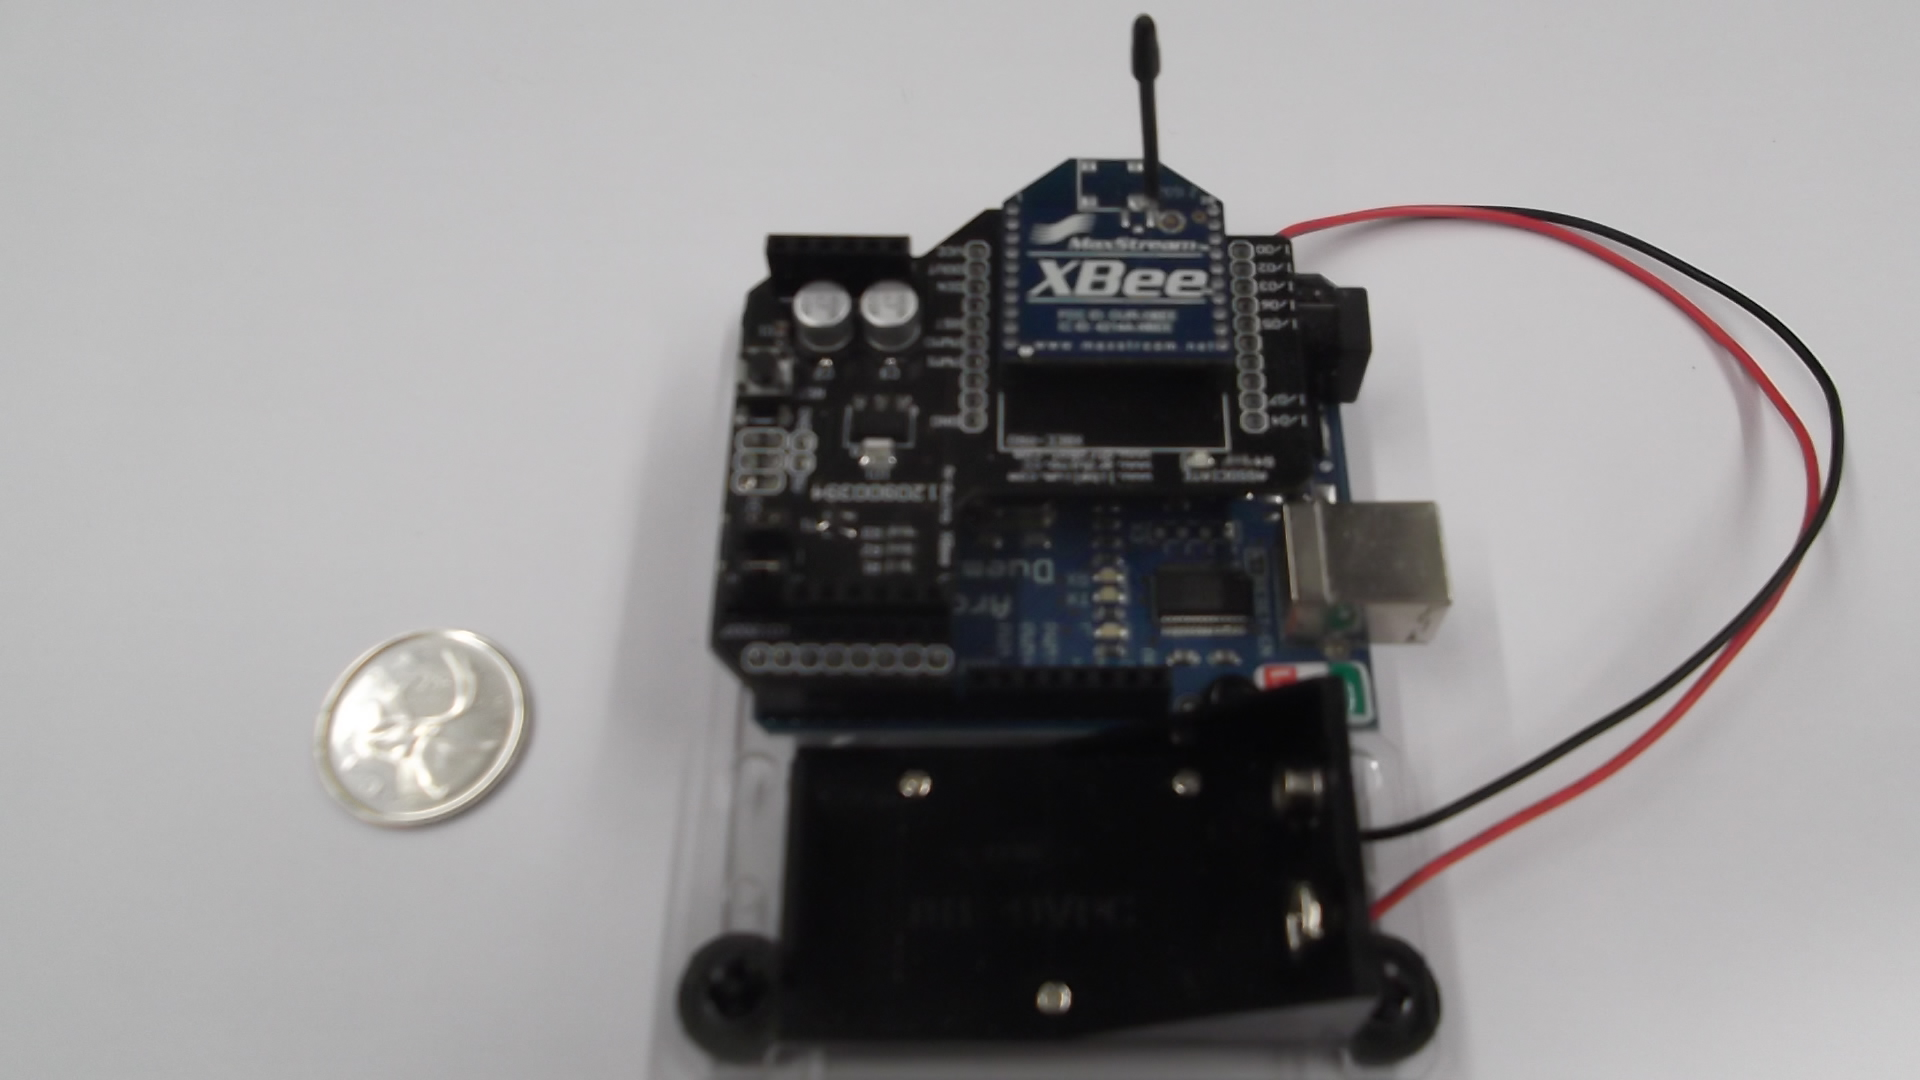
\includegraphics[height=3in]{images/motes/arduinoStack.jpg}
		\caption{An Arduino Duemilanove turned into a mote using the XBee Shield and an XBee radio.}
		\label{fig:images_motes_arduinoUnstack}
	\end{figure}
	
	\begin{figure}[\begin{figure}[htp]
		\centering
			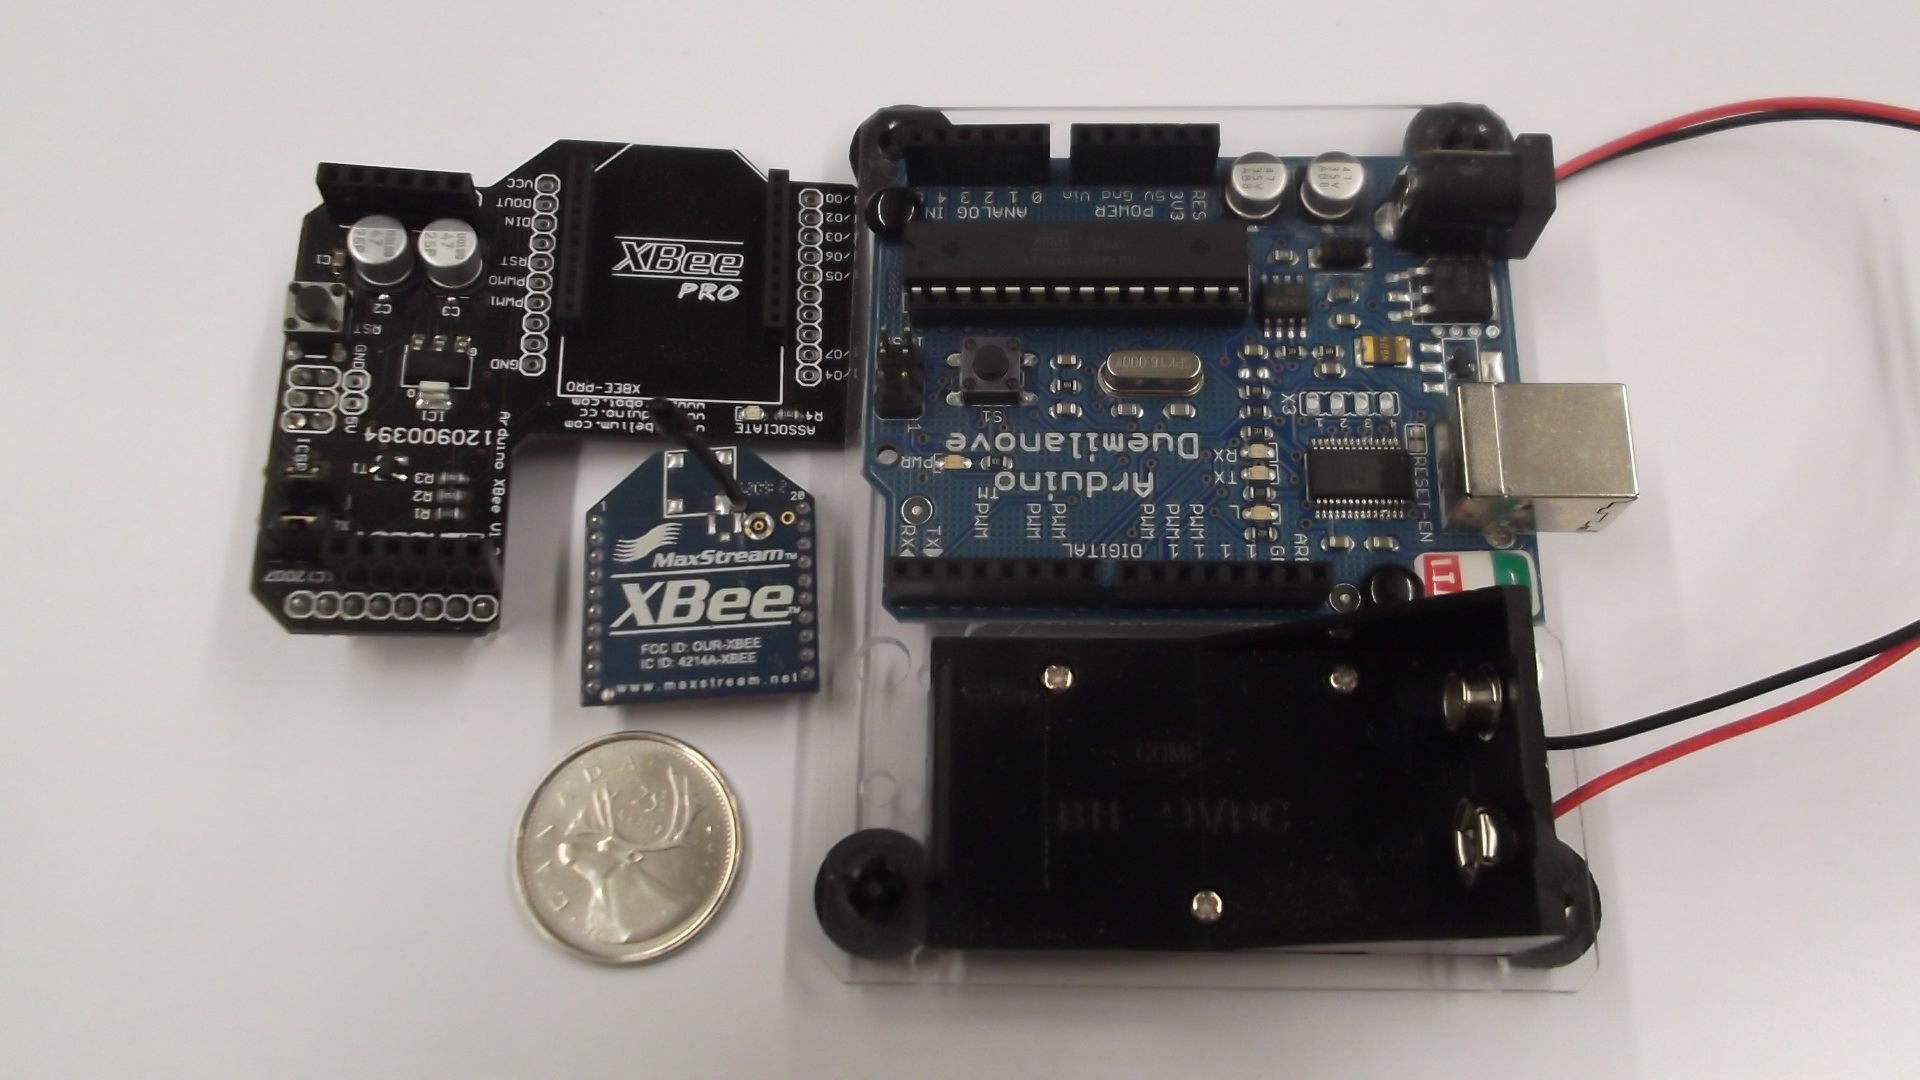
\includegraphics[height=3in]{images/motes/arduinoUnstack.jpg}
		\caption{The parts used to make the Arduino mote.}
		\label{fig:images_motes_arduinoStack}
	\end{figure}
	
	
	\paragraph{Possible modifications to the Stalker.}
    
    There is no battery packaged with the Arduino Duemilanove, so adding a battery is 
    necessary for the mote to work in the network. The Duemilanove is a custom 
    setup, and could be considered to be a heterogeneous mote by design.
    
    The Stalker ships with a button-cell battery that would not provide the stalker 
    with a very long lifespan. A larger battery would be necessary to make the Stalker 
    a useful mote.
		

	\paragraph{\emph{Uses for the Stalker and Arduino in a Heterogeneous WSN.}}
	
	The Stalker could be used for a routing mote, utilizing it's large
	storage capabilities provided by the MicroSD card. The Stalker could 
	also be used as a customized sensing node, using an Arduino-compatible 
	shield, or by using the Stalker's general purpose pins to connect to a sensor.
	
	\paragraph{\emph{Software used.}}
	
	Since the Stalker does not have a radio built onto the board, a third-party
	radio must be used. The Stalker provides an XBee-compatible port to host a radio.
	This XBee-compatible port uses the serial port on the Stalker board to contact the 
	radio. This works well with XBee radios, as they natively work in `transparent mode', which 
	means that the serial transmissions are sent over-the-air to other XBee radios
	in a way that the software using the radio need not know that a radio is being used.
	
	Since this project requires developing custom packets, a different mode must be used 
	when using the XBee radios to send and receive custom packets. The XBee Series 2, which
	is used in the experiment, has a mode called `API mode', that allows a developer to 
	create and read packets manually. A library named Arduino-Xbee~\cite{xbee-arduino} was 
	used to create and parse 802.15.4 packets properly. The library was modified to be
	more flexible and configureable to be more useful in the experiments.

\subsubsection {tMote Sky}
	The origins of the tMote Sky are from University of California, Berkeley. The basic 
	design is named Telos~\cite{telosOriginalPaper}, and has been marketed by several
	companies. The Telos mote was marketed by MoteIV, renaming it the tMote Sky.  
	MoteIV has been rebranded and renamed Sentilla. Sentill is still marketing the motes, as the Sentilla Mica.
	The motes have also been marketed as Crossbow, renamed to JCreate, all of which have a 
	similar design as seen in Figure~\ref{fig:images_motes_tmoteOneSide}.
	Each of these rebranded Telos motes have slightly different processors with 
	slightly differing memory sizes and sensors. The Telos variants are therefore 
	heterogeneous due to all of the different variants that are available.

	
	\paragraph{\emph{Possible modifications to the tMote Sky.}}
	The Telos mote has a large built-on power supply, and should not need a larger
	power supply. 
	The Telos does not have a large onboard memory, adding an external
	memory would make it a good router/clusterhead mote.
	
	%TODO - more? or move?
		
\begin{figure}[htbp]
	\centering
		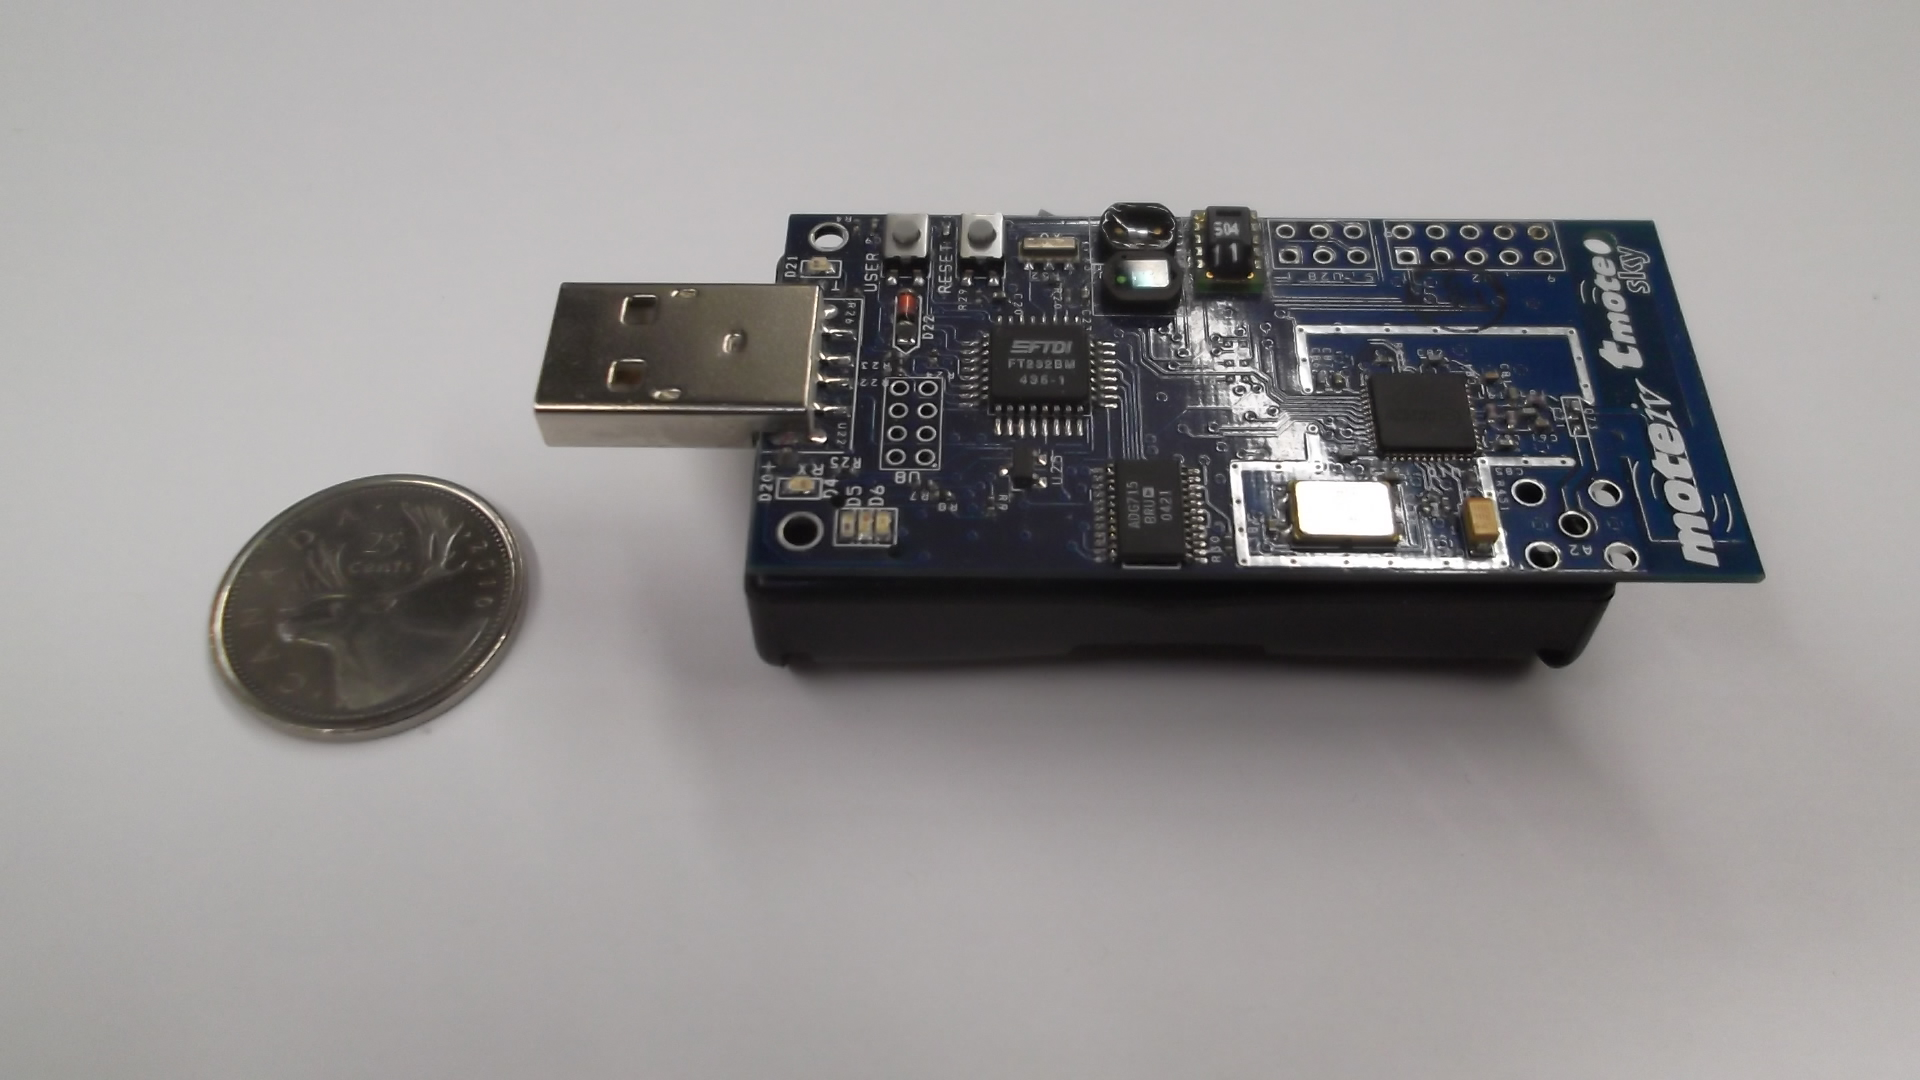
\includegraphics[height=3in]{images/motes/tmoteOneSide.jpg}
	\caption{The tmote Sky, which is a Telos variant.}
	\label{fig:images_motes_tmoteOneSide}
\end{figure}

	\paragraph{\emph{Uses for the tMote Sky in a Heterogeneous WSN.}}
	There are a number of onboard sensors making this a good mote for
	sensing tasks. Though, the large battery also makes the tMote a good candidate for 
	clusterhead, making the tMote a very versatile mote.
	

\subsection{Heterogeneous Setup of the Motes}	
Table~\ref{itsaTable} summarizes the motes, comparing the processors, radios, memory and battery power.
From the table it is easy to see the stark differences between the motes. The SunSPOT 
has a huge amount of memory and much more powerful processor than the
other motes, but its battery is tiny. The tMote has a
full operating system that is very easy to work with, and 
a large battery, but not a lot of flash memory. Though, the amount of flash memory is 
large in comparison with the Stalker and the Arduino which have almost no memory and very small extended memory.

Clearly, the SunSPOT is the most powerful mote in every respect except battery power. The tMote will take
the clusterhead head task the most frequently due to it's good extended memory size and battery power. The Stalker
and Arduino will not likely be clusterheads due to the limited extended memory which equates to limited 
queue sizes available on the devices.

While creating the testbed deployment, developing the  software for LEACH and HCCP on the 
Stalker was an issue, due to the very limited program space. Due to this, a minimalistic, chopped down
version of Contiki OS had to be made. The software uses the message queue code and interrupt callback code
from Contiki, while removing all other functions of the OS.
Contiki functions that were removed were any threads and context switching, drivers for sensors and  portability code 
so this version of Contiki can only run on Arduino microcontrollers.
This code was ported to the  Arduino with the ATmega 328 chip first, then an
even more stripped-down version had to be made for the Stalker with the less powerful ATmega 168p chip. 
The Stalker version of the software turns the
message queue into a ring buffer, and has limited roundtable abilities which only allow the Stalker to
accept routing information, and do nothing else during the Roundtable time.

Clearly, any of the modifications previously discussed could add more heterogeneity to this
already highly heterogeneous network if so desired.
	
\begin{table}
\begin{center}
\begin{scriptsizetabular}{|c|c|c|c|c|c|}
\hline
~ &  &  & & \textbf{Extended} & \textbf{OS /} \\
 & \textbf{Processor} & \textbf{Radio} &  \textbf{Memory} & \textbf{Memory} & \textbf{Software} \\
\hline
\textbf{SunSPOT} & 400 MHz 32-bit ARM920T & CC2420 & 1 MB & 8 MB & SunSPOT Framework \\
\hline
\textbf{tMote} & 8 MHz 16-bit TI MSP430 & CC2420 & 10 kB & 48 kB & Contiki OS \\
\hline
\textbf{Stalker} & 20 MHz 8-bit Atmel ATmega 168P & XBee Socket & 1 kB & 16 kB & Minimal Contiki OS \\
\hline
\textbf{Arduino} & 16 MHz 8-bit Atmel ATmega 328 & XBee Socket & 2 kB & 32 kB & Minimal Contiki OS \\
\hline

\end{scriptsizetabular}
\caption[Comparison of Motes in Testbed Deployment]{Comparison of Motes in Testbed Deployment.}
\label{itsaTable}
\end{center}
\end{table}
% http://arduino.cc/en/Main/ArduinoBoardDuemilanove/
% http://www.atmel.com/devices/atmega168p.aspx
% http://www.seeedstudio.com/wiki/Seeeduino_Stalker_v1.0
% http://www.sunspotworld.com/docs/index.html
% http://www.eecs.harvard.edu/~konrad/projects/shimmer/references/tmote-sky-datasheet.pdf
% 

\subsection{Testbed deployment}

To test the real-world feasibility of HCCP, a controlled physical deployment was run. 
SunSPOTs were used exclusively in the controlled deployment, as they were 
readily available in large quantities. A problem that plagued both  testbed deployments was that 
the SunSPOTs used were about five years old, and the rechargeable batteries that 
are built-in were starting to show signs of age. In the deployment, some of the motes
had the low battery warning light illuminated immediately despite being
fully charged. Due to the poor batteries, some of the motes
started dying after only 4 hours of running the experiment.
Due to the wear on the rechargeable batteries,
all the motes had a different amount of charge to use, which made the network
heterogeneous in terms of battery power. Adding different types of motes would
make the network more heterogenous, but the results would be very difficult to interpret due to the
amount of heterogeneity.



LEACH was set up as prescribed by Heinzelman et al.~\cite{leach} adding beacon routing information to the
Clusterhead Election announcement.

\subsubsection{House Monitoring Deployment}
\begin{figure}[htb]
    \centering
        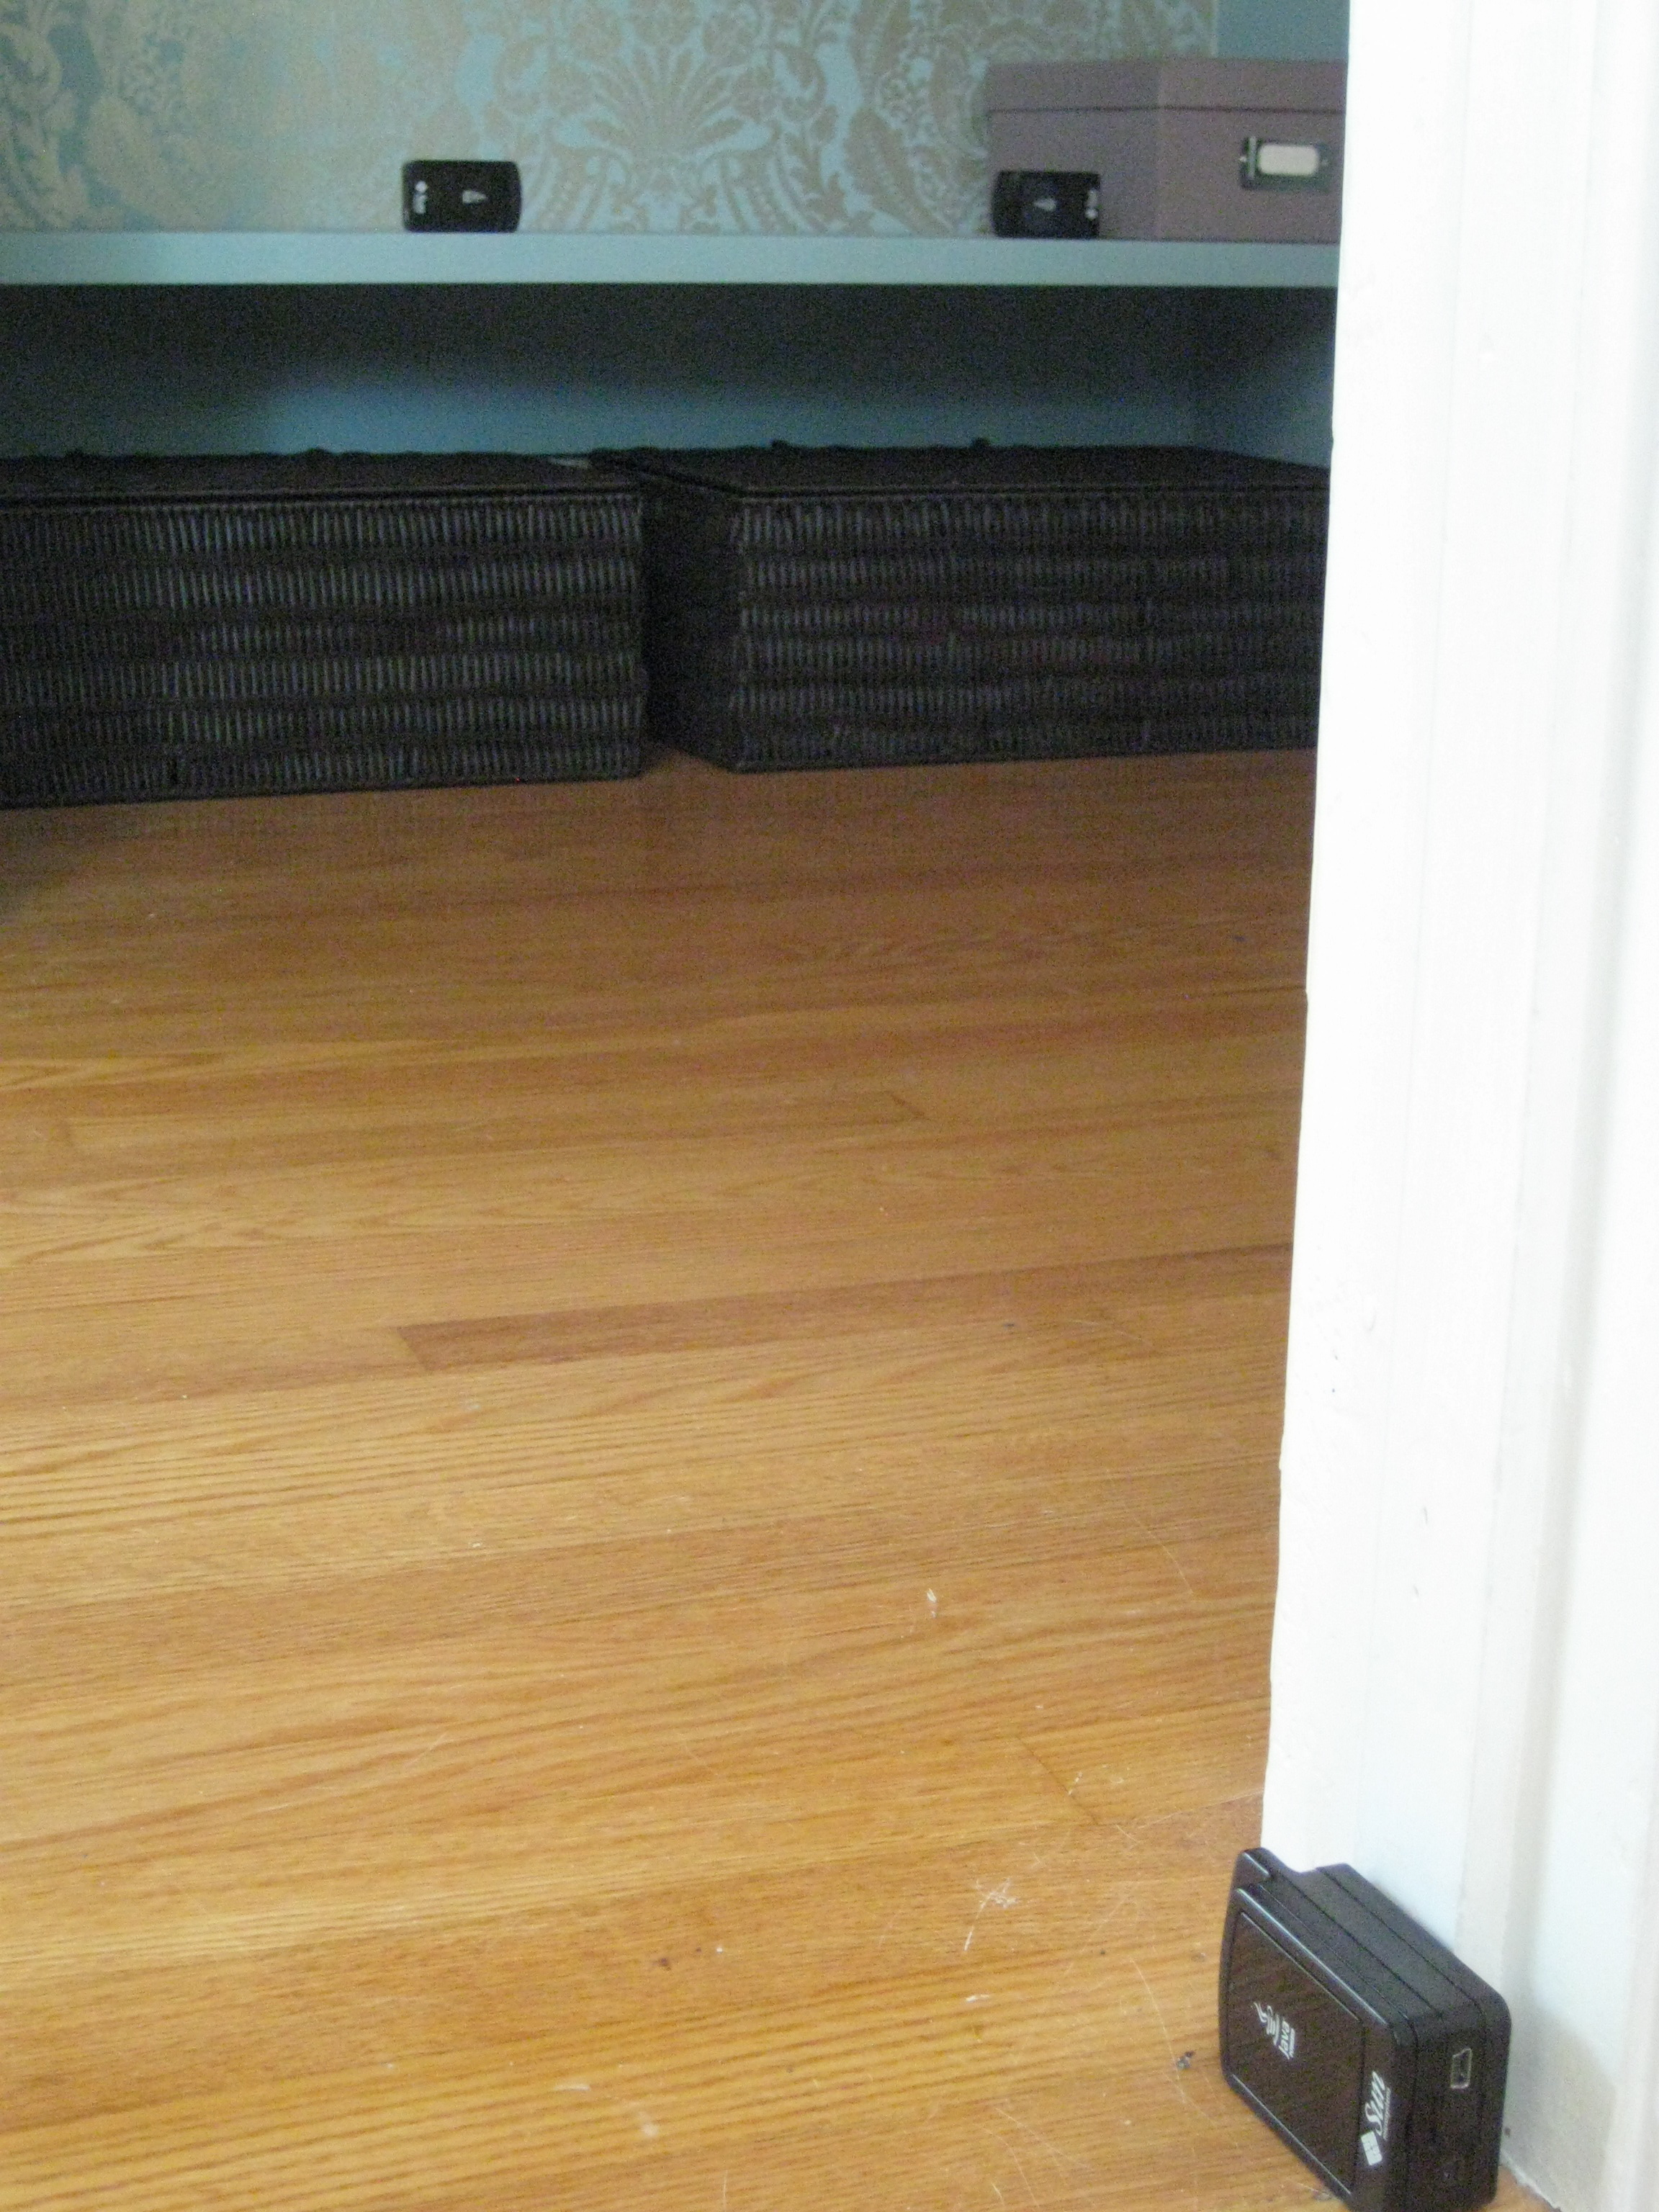
\includegraphics[height=5in]{images/deployment/hallway.JPG}
    \caption{Motes distributed around a house.}
    \label{fig:images_deployment_hallway}
\end{figure}

To show HCCP working in a real-world scenario, motes were distributed around a house.
Setting out motes around a house can simulate house monitoring for temperature, humidity
or even security. Motes could also be used in a house for home automation such as 
turning on lights in the room as a person enters, or having moving what's on television
from one room to the next as a person moves through a house.


The motes were deployed at various heights across a house as seen in Figure~\ref{fig:images_deployment_hallway}, with some motes placed outside
in waterproof containers. 
The networks had 44 motes and 1 sink distributed over (110) square meters (about 1200 square feet)
on various different levels and were made to communicate through various different materials.
The motes relayed their messages back to a sink that was placed centrally
in the house, this provided many routes back to the sink from any given mote. The motes were setup to create five new messages per minute, 
with all messages to be routed 
towards the sink.
Radio range was reduced to 4 meters line-of-sight to keep the network maintainable
and to ensure the network was a multi-hop network. Motes on the edges of the deployment were
setup to be at least three hops away.
The same network layout was used 
with both HCCP and LEACH deployments.


\begin{figure}[tb]
    \centering
        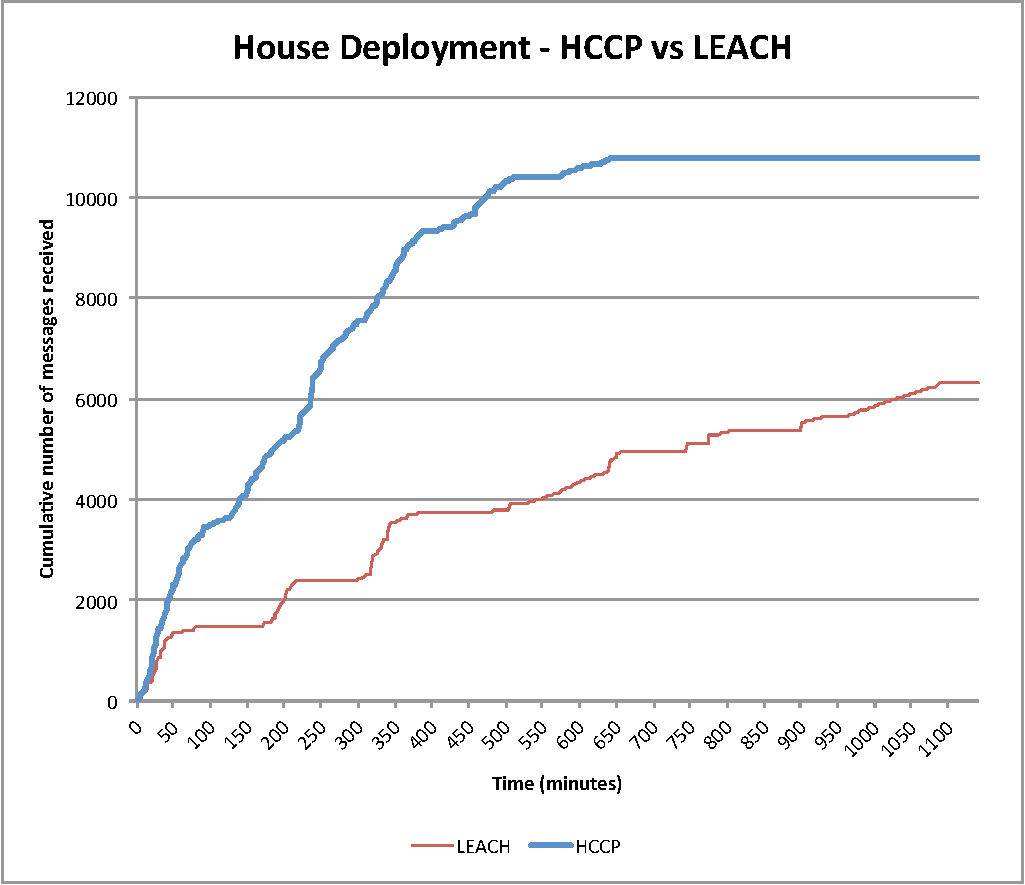
\includegraphics[width=5in]{images/deployment/houseResults.pdf}
    \caption{Cumulative number of messages received from the deployment done in a house.}
    \label{fig:images_deployment_houseResults}
\end{figure}

HCCP proved to be very effective at moving messages to the sink faster, as seen in Figure~\ref{fig:images_deployment_houseResults}.  
At 600 minutes (10 hours) the 
motes closest to the sink became inoperable, stopping the progress of the network.
Since the network was setup as quite sparsely,  a few motes dying early near the sink would have a large 
effect on the network. The performance of LEACH also degrades after the 600 minute mark, having received
62\% of its messages before the 10 hour mark.

Before the 10 hour mark, HCCP achieved approximately double the message throughput
that LEACH did. Also, HCCP had a much more consistent curve, creating a more linear chart. LEACH
has a step-function, probably due to the 5\% clusterhead rate as prescribed by Heinzelman et al.\ 
in their description of LEACH. Since the network cycle was setup to take one minute, messages can only 
flow into the motes next to the sink every 20 minutes, when the motes next to the sink choose to become clusterheads.

HCCP, on the other hand, was focused on Message Queue (95\%) and Battery Power (5\%). As the queues of the motes filled, 
they would be less likely to be clusterheads, allowing messages to to flow out of them. 
Then, as motes further away from the sink get full of messages, they 
are less likely to become clusterheads. As the motes further away
choose to be clusterheads less frequently, the motes close to the sink 
will more likely be clusterheads, which allows the messages flow 
towards the sink. As the motes close to the sink fill with messages from the motes further
from the also sink fill with messages, they will not be clusterheads as frequently, which
allows the messages to be sent to the sink.


\subsubsection{Grid Deployment}

\begin{figure}[htb]
    \centering
        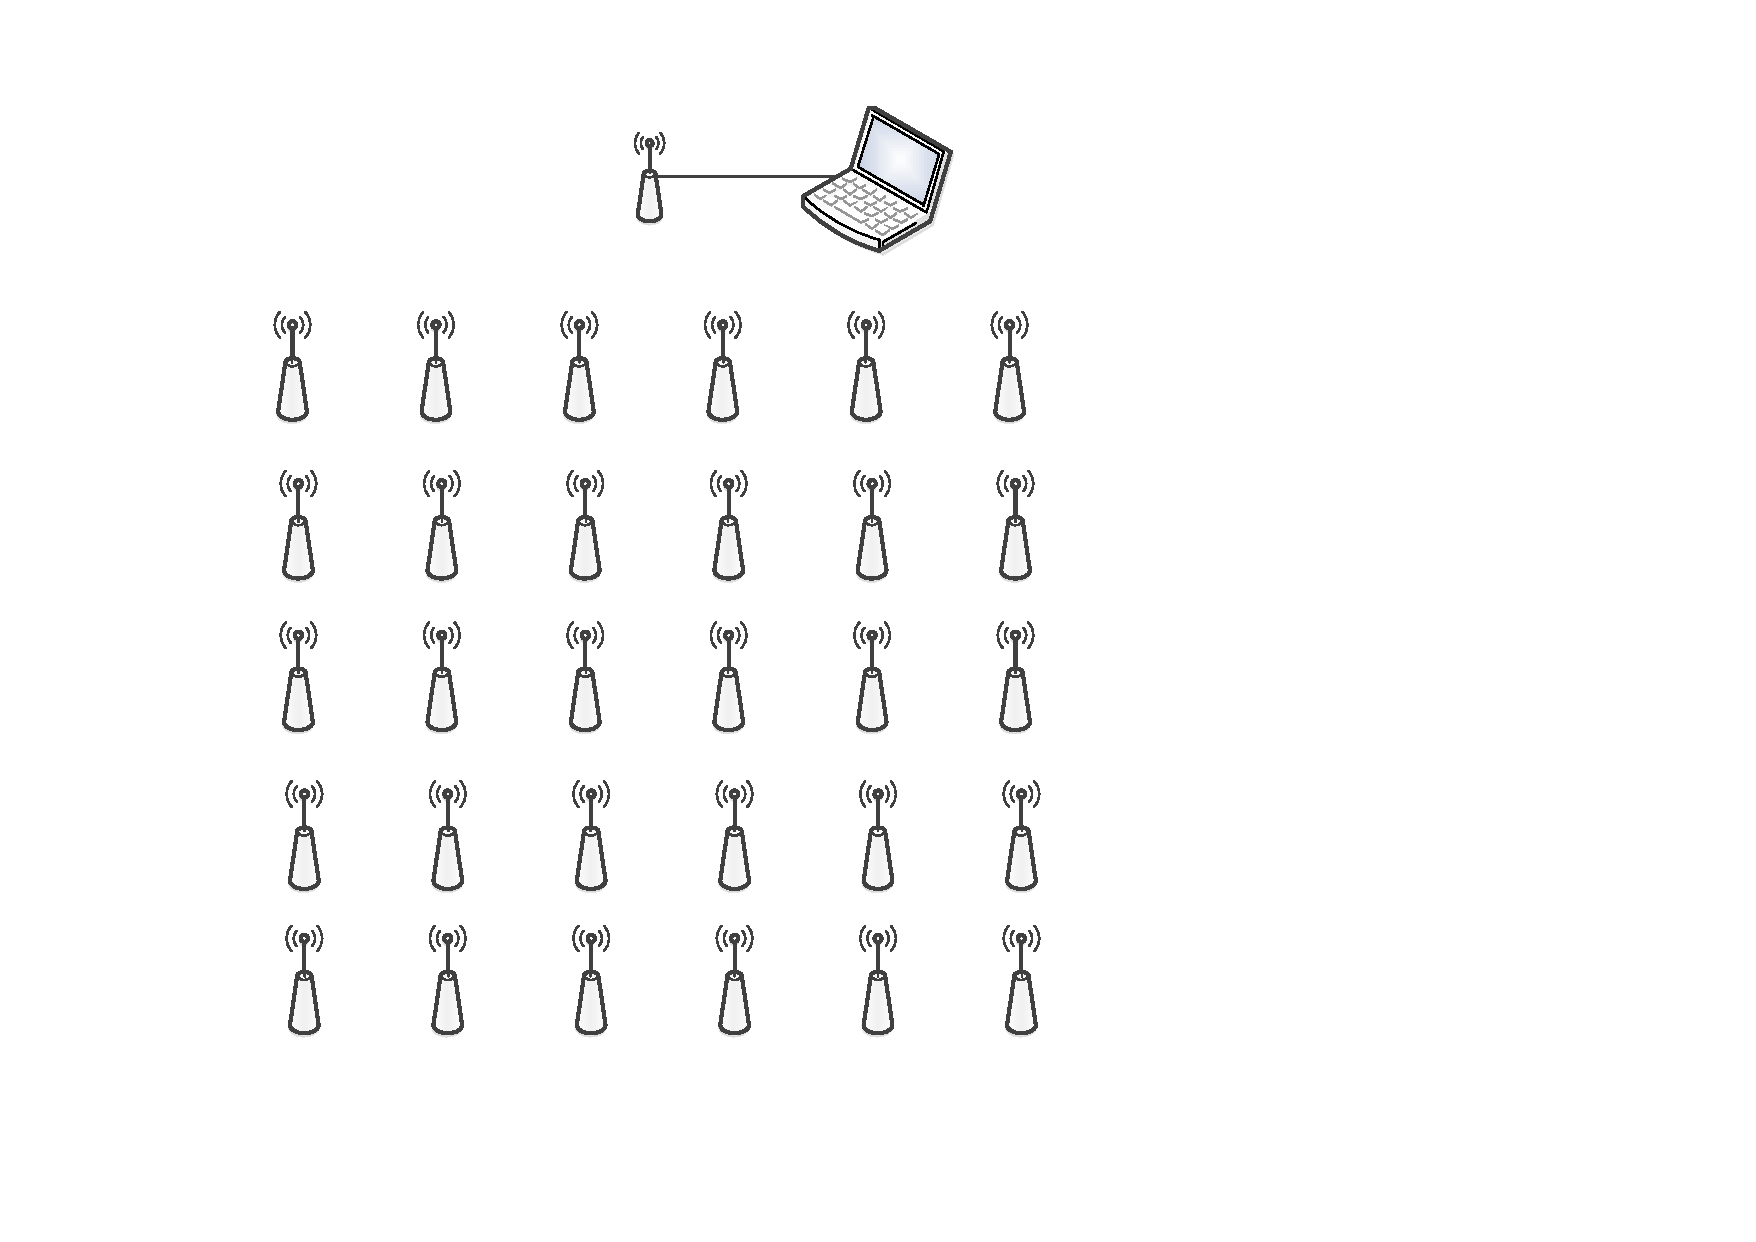
\includegraphics[height=3.5in]{images/deployment/gridChopped.pdf}
    \caption{The grid deployment setup.}
    \label{fig:images_deployment_gridChopped}
\end{figure}


A second deployment was done with 30 motes and a sink. The motes were set up in a 5 by 6 grid,
with 1.5 meter spacings between them. This made the grid spread out over a 7.5 meter by 9 meter 
area. The radio range was set to a 6 meter range, which will degrade over the lifespan of the network.
The sink was set up at the side of the network, as seen in Figure~\ref{fig:images_deployment_gridChopped}.

During both the LEACH and HCCP deployments, some of the motes immediately had the battery low warning light illuminated, 
despite the fact all batteries were fully charged before the deployment. Rechargeable batteries lose their ability to 
hold a charge as they age; since these are older motes it is only natural that some of the batteries would
be quite degraded. The motes that were nearly dead at time of deployment were left in the network for the test.

One problem about battery-powered devices is that as the battery drains, the device 
becomes unreliable. This unreliability stems from transistors not switching properly due
to not being able to draw enough current, or not having enough voltage to cause the
transistor to change state. Since the SunSPOT batteries were old, the motes were only reliable 
for about 10 hours. After 10 hours the motes could not maintain the network schedule, as 
the timer would not work properly. Interestingly, during the HCCP deployment, 
3 motes lasted over 60 hours but didn't send any messages during that time, meaning that the
motes were in deep sleep for that entire time. Not waking from sleep can happen when 
the wakeup timer never fires, leaving the mote asleep indefinitely.


\begin{figure}[tbh]
    \centering
        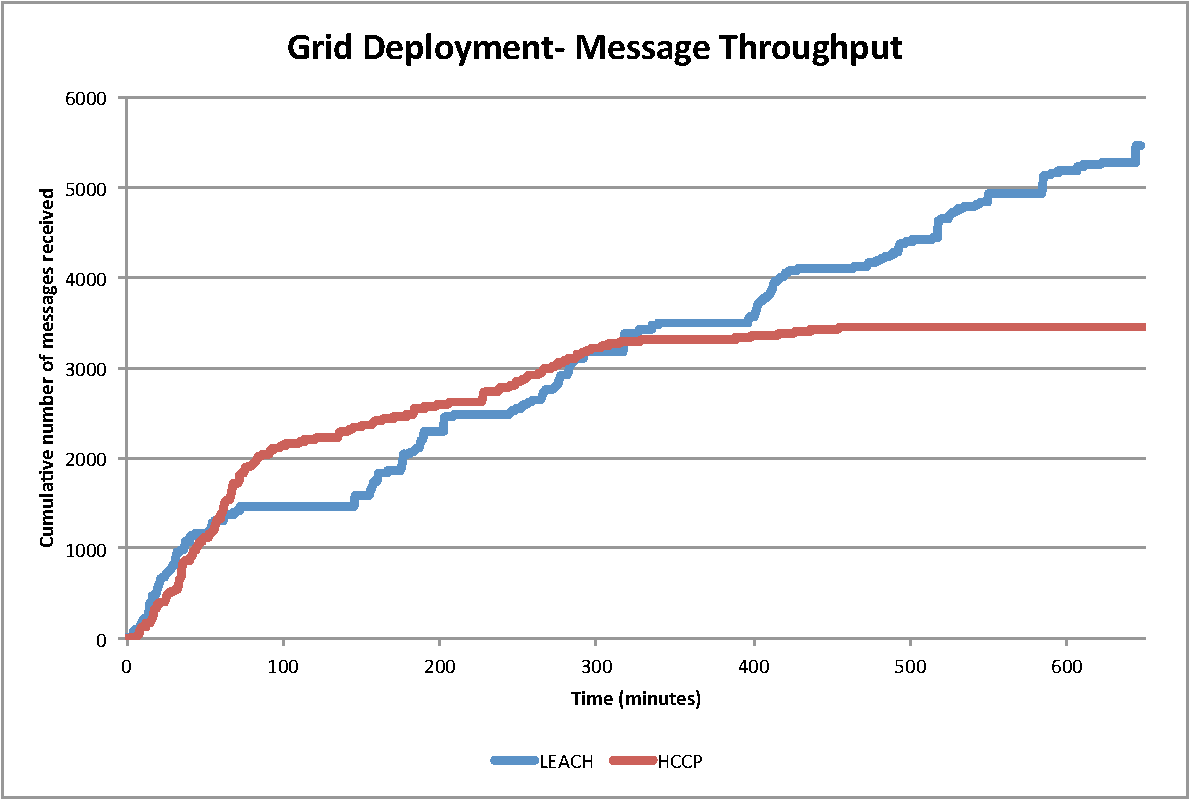
\includegraphics[height=3in]{images/deployment/results.pdf}
    \caption{Results from LEACH and HCCP Grid Deployments}
    \label{fig:images_deployment_results}
\end{figure}

The results from the grid deployment is shown in Figure~\ref{fig:images_deployment_results}.
At the start of the deployments, HCCP started with a better message throughput, as expected from
the results of the simulations. The throughput of HCCP then drops to a slower rate, allowing LEACH to 
catch up, and overtake it. HCCP then levels off, as motes begin to fail as the 300 minute (5 hour) point
approaches. Motes close to the sink were failing due to going to sleep, causing the messages to not have a
route to the sink.

The LEACH curve is more consistent than the HCCP curve, having steady steps. The
steps are quite interesting, as the LEACH network cycle was setup to take a minute, so the steps
should be in shorter cycles than 10 minutes.

If the motes had be provisioned with larger batteries, HCCP should maintain the slope it was forming before the 100 minute mark.
The HCCP deployment had the unfortunate luck of having the motes closest to the sink die first due to 
poor batteries, dying early of reasons unrelated to the protocol.

For network lifespan, the last message received in the LEACH network was at 646 minutes (10.75 hours). 
Since the motes closest to the sink in the HCCP deployment had problems waking from sleep, the 
last message was received at 3489 minutes (58.15 hours). This huge network lifespan is due to 
a mote rebooting after being in deep sleep for a long time, rejoining the network and sending it's 
messages to the sink. LEACH likely had motes do the same thing, but the motes weren't as close to the sink
and therefore did not create these odd data points.


Overall, HCCP has worked as a proof-of-concept in a real-world deployment. Since older motes were 
used, the results are difficult to interpret. Despite these difficulties, HCCP worked 
well, showing its real-world plausibility.
 






\chapter{Conclusion and Future Work}
\label{ch:conclusion}

In both simulation and testbed deployments, HCCP has increased message throughput while
having very little negative effects on network lifespan. HCCP provides 
a robust and tuneable network that provides many options to elect motes
that have certain properties as clusterheads more frequently. 
Depending on the configuration, HCCP appears to be able to provide network lifespans 
as long as LEACH while having almost double the message throughput, as shown in both 
simulations and physical deployments.

While HCCP is more complex than LEACH, it has a more robust design, and provides
infrastructure for disseminating information across the network. HCCP relies on 
the network to have schedules in tight synchronization, which is a
requirement in all WSN protocols, the novelty that HCCP adds is to 
use this highly coupled time to describe how good a
mote would be at being a clusterhead. The Goodness Delay
utilizes time that would otherwise not be used to optimize 
which motes will be clusterheads. 

HCCP is designed to be an easily tuneable protocol, giving 
the network designer tools to make the best network possible. 
An example of tuning the network is 
changing the length of the Roundtable Discussion time. This time
is allotted to share any network-specific information that 
doesn't fit anywhere else into the network. HCCP provides some suggestions
as to what to share during this time, but is intended to be customized 
for every individual network, or even left out if desired.

Heterogeneity in a WSN can be a powerful thing, and HCCP uses this
heterogeneity to elect better clusterheads. The definition of `better' is
up to the network designer to choose. HCCP allows the election to focus 
on motes that have qualities that a network designer feels are important 
to the network. This thesis provides insight into what heterogeneous 
factors have to offer to the network, how the affect the election, message
throughput and network/mote lifespans.

Overall, heterogeneity, whether the differences are small  or large, can be used 
to generate better functioning WSNs. Choosing motes that are better for the task of clusterhead 
will prevent lost messages with no cost to the lifespan of the network. The gains of 
using heterogeneity that is already inherent in every WSN is free, having few negative 
effects. Having the heterogeneity of a network self-assessed will ensure that 
as a network degrades over time that the best possible motes at that time will
be doing tasks that they are well-suited for, providing gains to the network from the time
it is deployed to the time the last mote ceases to function.

% future work

Looking forward, HCCP could be simplified for further energy savings. For instance,
the Clusterhead Candidacy phase could likely be merged with the Clusterhead Announcement phase,
as there is little difference to the network lifespan or message throughput when the phases are merged. 
Since removing the
Clusterhead Candidacy would make HCCP simpler and would not 
have any negative affects on the network, it would probably be a good idea. Further
research could done on how HCCP could surpass LEACH in terms of network lifespan.

A better routing protocol should be 
incorporated into the design of HCCP. More research could be done 
to see which routing algorithms would be the best with HCCP. The routing
algorithm should also take advantage of the heterogeneity of the network, routing 
messages through stronger motes.
HCCP was designed with this in mind, and is easily changed to use any routing algorithm. 
Further, if a mobile sink is a consideration, then using a routing algorithm that works efficiently with
networks that have a mobile sink, such as MobiRoute~\cite{mobileSinkRouting}, is also possible.

Querying motes in the network from the sink was not a focus of HCCP. If a network administrator 
wants to request data from a mote, there is no set method of sending the messages to any mote in the network
but the sink. To add querying to HCCP, a different routing method would need to be used, as only the  
sink's position is advertised while using beacon routing. A routing protocol that has a table
of all the mote's last known positions would need to be used. Once routing is set up, the 
querying framework would need to be added. This feature could be added into the 
Roundtable Discussion time, or into a new phase that is dedicated to mote querying.

HCCP was not designed with any inherent security measures. If messages are solely to be routed to the sink, 
simple RSA encryption~\cite{rsa}
could be used to encrypt the messages that are being sent to the sink. Other security issues such as
an errant mote that is dying continually becoming a clusterhead could be solved by blacklisting motes
that are continuously clusterheads.

To create a WSN with fewer collisions in the network,
it is possible to use Frequency Division Multiple access (FDMA)~\cite{fdma} to use
different radio channels for different clusters. 
Clusterheads could announce the channel along with the TDMA schedule. 
Using multiple radio channels during the TDMA clustermote reporting run time would remove many of the collisions
that happen during the TDMA run time.


Radio power could also be adjusted to suit the size of the network. Adjusting the radio power to the lowest transmission
power saves mote energy, and prevents motes from flooding the network with unecessary messages from motes. Also, smaller transmission 
ranges make clusters smaller. Changing the radio power effectively changes the cluster size, since few motes will be in 
range. 
Lin et al.~\cite{atpc}, Zheng et al.~\cite{adaptive2010}, Xiao and Yu~\cite{efficientRadioPower} and others have 
developed efficient methods of adjusting the radio power to enable motes to talk 
to a limited number of neighbouring motes. Messages to communicate radio power could be added
to the HCCP's Roundtable Discussion, or piggybacked on announcement messages, such as clusterhead announcements.


\section{Future Goals of WSNs}


Smart Dust~\cite{smartdust-2, SmartDust-NC}, is one of the potential futures for WSNs. As circuits, processors
and motes get smaller and smaller there may come a point where motes are no larger than the size of dust.
These motes would have near negligible unit cost and be deployed in the thousands. Smart
Dust would communicate wirelessly, monitoring some phenomena and glean energy from the environment
to stay powered. Smart Dust would need to be deployed with a dense network that would need to be a multi-hop 
network, as each device would have minimal battery power and minimal transmission power. Any protocols designed
would have to be scalable to accommodate large networks of Smart Dust. HCCP has been designed to scale, but 
smart dust might be a larger scale than HCCP was designed for, though HCCP provides interesting ways
to use the differences in the dust well.

As devices get smaller and more feature-rich, the eventual outcome might be
that all devices are networked and can communicate with each other. When all devices
can communicate with each other, they would create `an internet of things', a term 
used frequently by Adam Dunkels~\cite{vasseur10interconnecting}, who is the 
creator of Contiki OS~\cite{dunkels04contiki, contikiOS} and a key member of the WSN community.
Dunkels et al.~\cite{dunkels11adhoc} believe that devices will communicate with each other using a
lightweight version of IPv6 called 6LoWPAN IPv6~\cite{jhui10ipv6}. A subset of the larger IPv6 protocol~\cite{ipv6} 
is an obvious choice, as it can provide unique addresses
for $3.4 \times 10^{38}$ devices, which would provide 
%$4.8 \times 10^{28}$ 
48~000~000~000~000~000~000~000~000~000 addresses
for every one of the 7 billion 
humans on Earth. This means that every single device in the Internet of Things could have 
it's own address, and be able to communicate with any other device in the internet of things. 
This would make the entire Internet a massive scale WSN of sorts, with many heterogeneous 
devices all connected using the common language of IPv6. HCCP uses IPv6 addressing, allowing 
networks running HCCP to possibly be part of the internet of things.




%\include{FutureWork} % merged with conclusion


% Appendices:list your appendix latex files you want included here, in order
%\appendix
%

\chapter{Supporting Data}
\label{ap1:data}
This is the Appendix showing Supporting data.

Check out these great graphs!




% bibliography: this assumes the bibtex file containing your bibliography information is named 'bibs.bib'...


%this uses the abbreviated names style - change to plainnat if you want names as they are verbatim in your bibtex
%see the included natbib documentation (included) if you want to create your own bibliography style other than these.

% part of the check for uncited stuff
%\nocite{*}


\bibliographystyle{unsrt}
\addcontentsline{toc}{chapter}{\bibname}
\bibliography{bibs} 
\end{document}
